

\documentclass[12pt,double,openany]{book}
\usepackage{setspace}
\usepackage{nameref}
\usepackage{amsthm, amsmath, amssymb, multirow, cite, comment, bm, array, mathrsfs} %graphics
\usepackage{graphicx , color, subcaption} %wrapfig, subfig, 
\usepackage{caption}
%\usepackage[font=scriptsize]{caption}
\usepackage{tikz} 
\usepackage{slashbox}
\usepackage[ruled,vlined]{algorithm2e}
\usepackage[nottoc,notlot,notlof]{tocbibind}
\graphicspath{{Images/}} 
\usepackage{pict2e}
\usetikzlibrary{arrows}
\doublespacing
\setlength{\textwidth}{6.5in}
\setlength{\textheight}{8.5in}
\setlength{\evensidemargin}{0in}
\setlength{\oddsidemargin}{0in}
\setlength{\topmargin}{0in}

\setlength{\parindent}{0pt}
\setlength{\parskip}{0.1in}



%\define \BLACK{black}
%\define \RED{red}
%\define \GREEN{green}


%\newcommand{\BLACK}{black}
%\newcommand{\mycolor}{\color{blue}} 

% Uncomment for double-spaced document.
% \renewcommand{\baselinestretch}{2}

% \usepackage{epsf}

\begin{document}
%\begin{document}
%	\pagestyle{plain}
%	%%---------------------------------------------------------------------------%%
%	\frontmatter
%	
%	\include{front}
%	
%	%%---------------------------------------------------------------------------%%
%	\mainmatter
%	
%	
%	
%	\pagestyle{plain}
%	\newgeometry{margin=1in,lmargin=1.25in,footskip=\chapterfootskip, includehead, includefoot}
%	\include{Chapter-1/Chapter-1}
%	\include{Chapter-2/Chapter-2}
%	\include{Chapter-3/Chapter-3}
%	%\include{Chapter-4/Chapter-4}
%	%\include{Chapter-5/Chapter-5}
%	%\include{Chapter-6/Chapter-6}
%	%\restoregeometry
%	
%	
%	%%---------------------------------------------------------------------------%%
%	%%  Bibliography 
%	
%	%%  You can use the bibitem list.
%	%\bibliographystyle{unsrt}
%	%\begin{%thebibliography}{99}
%	%\bibitem{cb02}
%	%Casella, G. and Berger, R.L. (2002)
%	%\newblock {\it Statistical Inference, Second Edition.}
%	%Duxbury Press, Belmont, CA.
%	%
%	%\bibitem{t06}
%	%Tsiatis, A.A. (2006)
%	%\newblock {\it Semiparametric Theory and Missing Data.}
%	%Springer, New York.
%	%
%	%\end{thebibliography}
%	
%	%% or use BibTeX
%	%\bibliography{Ortiz-thesis}{}
%	%\bibliographystyle{plain}
%	%\nociterec{*}
%	
%	%\bibliographystyle{plainnat}%plainnat is necessary to enable the use of citet. Natbib style file.
%	%\bibliography{Ortiz-thesis2}
%	%\ensureoddstart
%	\begin{spacing}{1}
%		\setlength\bibitemsep{11pt} %22pt = 2*11pt, where fontsize is 11pt
%		\phantomsection
%		\addcontentsline{toc}{chapter}{{\uppercase{\bibname}}} %\textorpdfstring and \uppercase needed due to hyperref package http://www.latex-community.org/forum/viewtopic.php?f=44&t=16601
%		%\vspace{-0.5in}
%		\titleformat{\chapter}[display]{\bf\filcenter
%		}{\chaptertitlename\ \thechapter}{11pt}{\bf\filcenter}
%		\titlespacing*{\chapter}{0pt}{-0.5in-9pt}{22pt}
%		
%		\printbibliography[heading=myheading]
%	\end{spacing}
%	%\bibliographystyle{apalike}
%	
%	
%	%%---------------------------------------------------------------------------%%
%	% Appendices
%	%\ensureoddstart
%	\restoregeometry
%	\appendix
%	\newgeometry{margin=1in,lmargin=1.25in,footskip=\chapterfootskip, includehead, includefoot}
%	
%	
%	\include{Appendix-A/Appendix-A}
%	
%	\restoregeometry
%	
%	%%---------------------------------------------------------------------------%%
%	%\ensureoddstart
%	\backmatter
%	
%	
%\end{document}
	\pagestyle{plain}
	%%---------------------------------------------------------------------------%%
	\frontmatter
\thispagestyle{empty}
\pagenumbering{roman}
%\begin{center}
	
	% TITLE
	{\Large 
	Predictive Modeling of ECG Signal Using Spatial Topology Based Feature Space Transformation
	}
	
	\vfill
	
	By Jiaming Chen
	
	\vfill
A Thesis	
Submitted in Partial Fulfillment\\
of the Requirements for Degree of \\
Master of Science\\
 in Electrical Engineering

	\vfill
	Northern Arizona University\\
	July 2018
	\vfill
	Approved:\\
	Abolfazl Razi, Ph.D, Chair \\
	Fatemeh Afghah, Ph.D\\ 
    Bertrand Cambou, Ph.D	

	
\end{center}
%
\begin{center}

\vfill

{\large Predictive Modeling of Biomedical Signal based on Spatial Topology Based Feature Space Transformation }

Jiaming Chen

{(ABSTRACT)}

%\vfill



\vfill

\end{center}
Biomedical signal classification has been frequently investigated by researchers in the past decades. Various classification systems have been proposed and evaluated by classification metrics. The essence of most methods, is to analyze test signals using reference models constructed based on a collection of healthy and abnormal signals. While system performances in terms of classifying signal samples increased significantly with modern machine learning algorithms such as recurrent neural network, there are one important factor in biomedical signal processing which is rarely studied in recent research.  In this work, we go one step beyond the conventional methods and intend to predict potential upcoming abnormalities before their occurrence. The approach is to build a patient-specific model and identify minor deviations (e.g. yellow alarms) from the normal trend, which can be indicative of potential upcoming significant deviations (red alarms). 

To facilitate a sound deviation analysis, a controlled spatial transformation is proposed to reshape the signal geometry in the feature space, such that the abnormality classes symmetrically surround the normal class. We applied the developed technique to Electrocardiogram (ECG) signals and the results confirm the utility of the proposed method in predicting upcoming heart abnormalities before their occurrence. For instance, the probability of a red alarm of specific abnormality class increases by 10\% after observing a yellow alarm of the same type. This approach is general and has the potential to be applied to a wide range of physiological signals.



% 
% \chapter*{Acknowledgements}
I would like to express my sincerest appreciation for %my advisor, Dr.Razi. Thank you for all of the advice, guidance, and patience. This accomplishment would never have been possible without the support you have provided for me. 
 
 %Thank you Dr.Afghah and Dr. Cambou for taking the time to be on my committee, and for all the advice.
 
 %Thank you to everyone at the wireless networking and information processing lab for the laughs and late nights. 
%\tableofcontents
%\listoffigures
%\newpage
%\vspace*{4cm}

%\centerline{\fontfamily{calligra}\selectfont \begin{large}  To my family\end{large}}
%\clearpage
\mainmatter
\pagenumbering{arabic}
%\pagestyle{myheadings}



% \chapter{Introduction}

 \section{Background and Motivation}
 
In the last decades, mortalities caused by heart diseases has been increasing sharply as a result of aging of population, chronic cardiovascular diseases, increasing life stress and continuously accelerating pace of life\cite{mortality}. According to heart disease and stroke statistics, cardiac diseases are the most common cause of sudden cardiac death (SCD) which leads to 250 000 to 300 000 mortalities in U.S. every year which accounts for 14.7\% of total deaths\cite{SCDnumber}. As World Health Organization reported, 31\% of global deaths are related to cardiovascular diseases (CVDs)\cite{who}. % Therefore, heart disease is called as “Plague of The Times”. In China, there are about 540,000 sudden cardiac deaths every year.In addition, heart diseases tend to attack younger generations, manifested by the increasing proportion of young patients.
These facts fully reflect that heart diseases are threatening the general health of human beings. Meanwhile since SCD can occur, most likely, without warning and apparent symptoms in advance, the prediction and early recognition of cardiac disease are considered challenging\cite{circulation2010}. Therefore it is of important significance to treat heart diseases timely by early detection and prediction of CVDs. 
While most CVDs are accompanied with arrhythmia, accurate and timely recolonization of arrhythmia is a key factor for preventing the incidence of heart diseases effectively and determine definitive therapies for CVDs.

Electrocardiogram (ECG),recorded for the first time by Waller in 1887, contains abundant physiological and pathological information that reflects the heart rhythm and status of various parts of the heart\cite{besterman1979waller}. %a professor of physiology at Queen Mary Hospital of Royal Society, by using the capillary electro-meter on hearts of dogs and human in 1887.
 ECG records signals generated by electrical activities of heart as a time series. As a noninvasive examination method, it is known to be highly reliable in reflecting functionality of heart. For this reason, ECG has become one of the most conventional technologies (ECG, clinical examination, radiation and ultrasonic inspection) in modernized hospitals and clinics, serving as an important reference for doctors’ diagnosis of heart diseases.


The traditional diagnosis based on ECG analysis are mainly accomplished manually by physicians. %According to working experiences and rich knowledge in heart diseases, experts observe and analyze ECG waveforms visually and make accurate diagnosis. 
However, this becomes costly and impractical when continuous monitoring for CVDs is required. There are tremendous ECG records generated everyday, all demand for timely diagnosis and analysis. Facing with the severe shortage of physicians, automatic ECG classification system is introduced to generate real-time analysis result and provide additional information to physicians. 

Automatic classification algorithms has been frequently investigated by researchers in the last decades. Whereas applying conventional classification algorithms on biomedical signals remains challenging, especially for applications of spontaneous disease detection. 

%0959-4965%
A typical feature of cardiovascular disease is its spontaneous occurrence. This unpredictability is the principal cause of high mortality for patients with heart disease. An informative anticipation of abnormality would enable a therapeutic intervention ahead of mortal occurrence and thus minimize risk of mortality. Nevertheless, the majority of developed conventional ECG classification systems haven't focused on real-time or predicting performance. %To address these problems, we propose in this thesis novel non-linear transformation based classification systems with the capacity to predict abnormality.

Another important character of ECG waveform is its variability caused by distinct physical conditions of different individuals (i.e. gender, age, body-mass index etc.)\cite{agesex}\cite{intervaria}. Conventional classification algorithms fall short of generalization when applying on different patients' records\cite{llamedo2012automatic}. Due to the inter-patient variation in ECG signals and the complexity of cardiac pathological information analysis, most of the existing ECG analysis software only serve as auxiliary devices for physicians. The final results of diagnosis still depend on manual labeling by cardiologists. %More importantly, the diagnostic accuracy of the automatic analysis system of the ECG signal still cannot reach the highest diagnostic accuracy of the clinician.

The automatic analysis of ECG signals incorporates a wide range of techniques. In this work, we focus on overcoming the two drawbacks of existing automatic ECG classification systems, which is patient-specificity and predicting capacity. This research aims at improving the inter-patient classification performance and predicting capacity of automatic analysis and recognition of arrhythmia with ECG signals, which has significance in efficient early detection of CVDs and reduce mortality rate of SCD. 

\section{ECG and Arrhythmia}

Electrocardiogram is widely used to monitor the electrical activities of heart and assist diagnosing fatal cardiac disease. In order to design algorithms specifically for ECG analysis, it's important to develop a insightful perception of the functionality of heart and ECG waveform.  

\subsection{Characteristics of ECG signal}

ECG signal reflects the periodical electric signals generated by heart. Fig.\ref{fig:cardiac_cycle} demonstrated the typical signal waveform for a cardiac cycle (i.e. a heartbeat), which is usually composed of three main waves: P wave, QRS complexes and T wave. These waves corresponds to different physiological activities of heart. P waves are generated by atrial depolarization which standards for the process of pumping blood to ventricles. QRS complexes as the most significant electric activities is caused by ventricular contraction meaning the process of pumping blood to lungs and the rest of the human body. Finally, T waves is the result of ventricular repolarization recovering this process at the end of a cardiac cycle. Accurate detection and segmentation of each waves are necessary for ECG analysis. The waves are usually localized at the peak of waves, these peaks are also called fiducial peaks. By detecting the most significant peak within QRS complexes: R peak, automatic algorithms are able to draw boundaries between cardiac cycle. The interval between two R peaks is called RR interval, which is also the inverse of heart rate.

\subsection{MIT-BIH Arrhythmia Database}

Arrhythmia is related to various of morbid behavior of heart. Generally speaking, arrhythmias consist of two main categories: supraventricular and ventricular. Ventricular ectopic beats imply abnormal activities in the ventricles while Supraventricular ectopic beats are related to the atria. Both categories contains fatal abnormal beats which may lead to death. Therefore, in order to help researchers standardize the evaluation of works on ECG classifiers, Association for the Advancement of Medical Instrumentation (AAMI) \cite{aami} has proposed recommendations for reporting ECG classifier performance. 
According to these recommendations, MIT-BIH Arrhythmia Database (MITDB) is regarded as the standard database to train and test ECG classifiers in the last decades. MITDB is a public database which is available on Physionet.com \cite{physionet} since 1997\cite{mitdb}. There are 48 records collected from 47 individuals in the database. Each record contains two channel of ECG raw signals together with annotations composed of 16 types and R peak locations provided by cardiologists. The sample frequency of MITDB is 360Hz and signal frequency spans from 0.1 to 100 Hz. 

Following the recommendation by AAMI, the original annotations of MITDB are further grouped into 4 major classes: class N(normal and bundle branch block beat types) class V(ventricular type), class S(supraventricular type) and class F(fusion of normal and ventricular types). The class Q which includes unclassified and paced beats are discarded due to the limit number of samples. Table.\ref{table:grouping_types} summarize the mapping from 16 original types in annotation to the standard 5 types recommended by AAMI:

\begin{table}[h]
\centering
\caption{Mapping from 16 original types in annotation to the standard 5 types recommended by AAMI}
\label{table:grouping_types}
\begin{tabular}{|c|c|}
\hline
Standard Types by AAMI & Original Types in MITDB Annotation \\ \hline
N                      & NOR, LBBB, RBBB, AE, NE            \\ \hline
V                      & PVC, VE, VF                        \\ \hline
S                      & APC, AP, BAP, NP                   \\ \hline
F                      & VFN                                \\ \hline
Q                      & PACE, FPN, UN                      \\ \hline
\end{tabular}
\end{table}



%For the purpose of training and evaluating classifier, MITDB is split into test (DS2) and training (DS1) set by balancing the four classes according to \cite{autofs}. 

\section{Problem Statement}

ECG signals, as a non-invasive method, are investigated broadly by researchers to design automated analysis and real-time monitoring systems. In the past decades, various ECG automatic analysis systems are proposed. As described in the last sections, there exists two main challenges: inter-patient variability and requirements for early detection and prediction. %To address these problems, we propose in this thesis two novel nonlinear transformation based patient-specific classification systems with the capacity to predict abnormality.

For conventional classification system, the training data is composed of records collected from different patients with annotations per heartbeat. In order to unify the records from different patients, most of the algorithms using conventional classification algorithm concatenate heartbeats from different records and thus result in a pooled ECG dataset. Since the classification performance is measured based on generated labels for each sample, the classifiers are trained to improve the performance on pooled ECG data. While ECG signals shares similar morphologies, the signals from different patients demonstrate considerable variance as shown in Fig.\ref{fig:interpatient_variability}. Ignoring this difference will lead to inconsistent classification performance between patients. Therefore it's of significant importance to adjust classifier configuration according to patient-specific characteristics.  %A patient-specific classification system refers to systems with cert

 \begin{figure}[thpb]
 	\centering
 	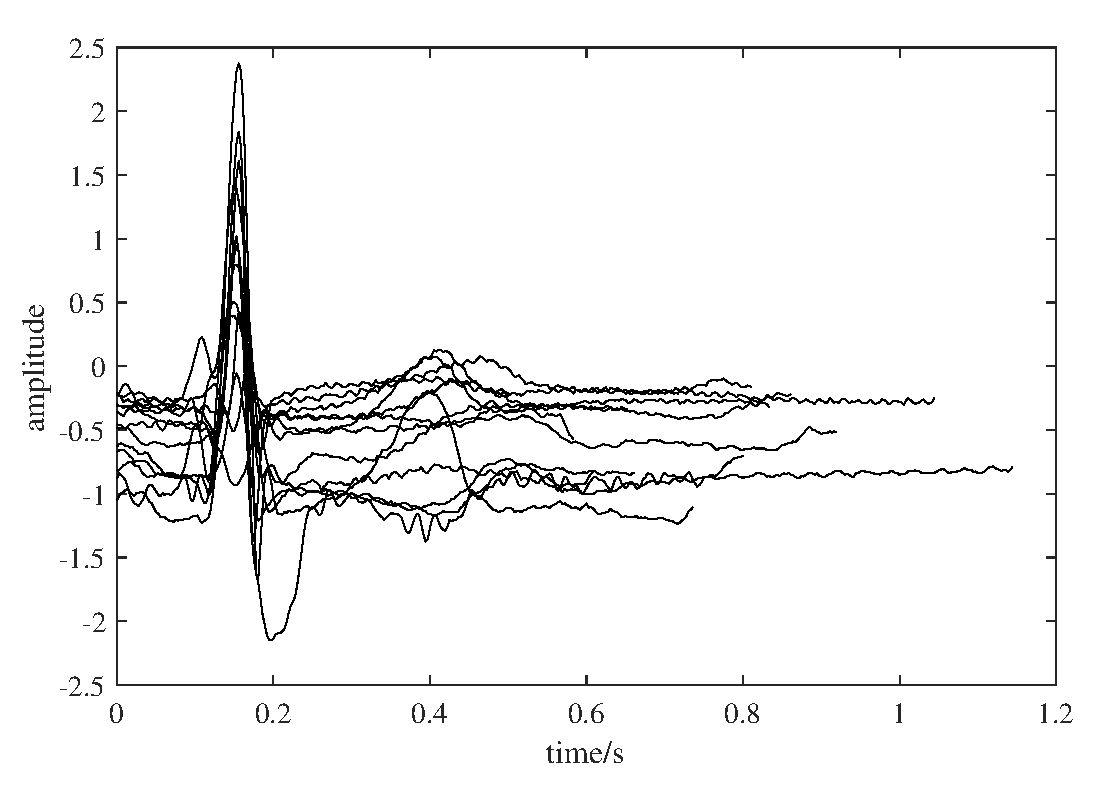
\includegraphics[scale=0.7]{Fig/interpatient_variability.pdf}
 	\caption{ECG signals of normal heartbeat from 15 different records reflect the inter-patient variability of ECG signal}
 	\label{fig:interpatient_variability}
 \end{figure}

In addition to the inter-patient variability, majority of ECG classification algorithms fail to consider the predicting capacity, which refers to the capacity of triggering corresponding alarms before the occurrence of abnormalities. By comparing the morphology of signals which shows salient similarities to abnormal signals precedent to morbid heartbeats with annotated abnormal signal, the potential latent status between abnormal and normal signals is partially demonstrated. If abnormalities in cardiologist annotation are represented by red alarms, thus a system which is able to trigger a corresponding yellow alarm precedent to the abnormality can be considered as capable of predicting abnormalities as shown in Fig.\ref{fig:pred_signals}. Therefore, a method to quantify the level of signal similarity to abnormalities should be incorporated in ECG classification system.

 \begin{figure}[t]
 	\centering
 	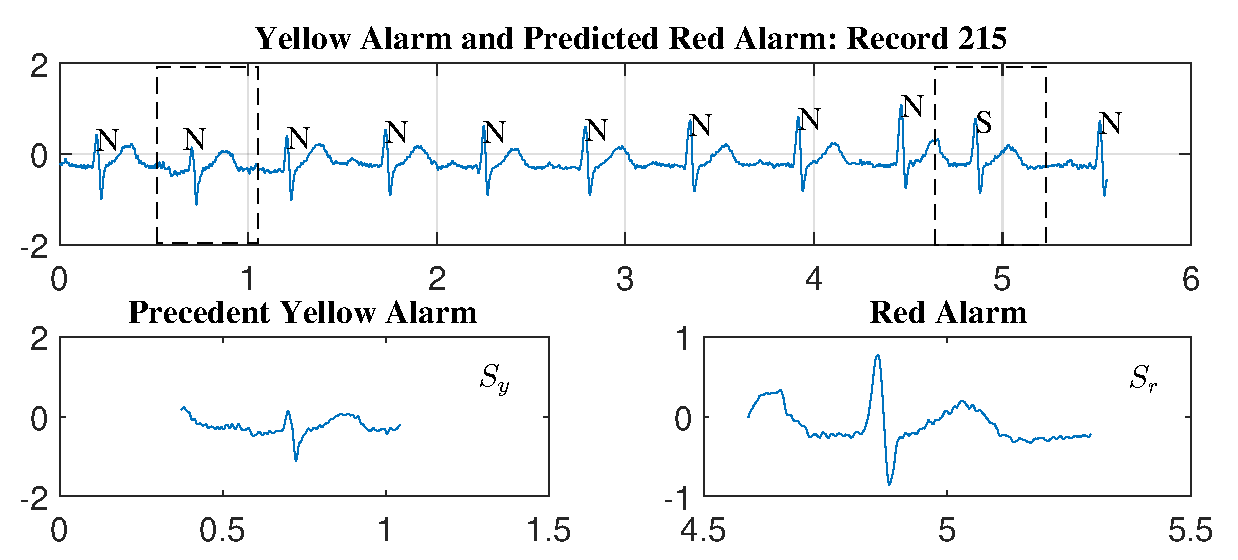
\includegraphics[scale=0.6]{Fig/predicting_record215S_croped.pdf}
 	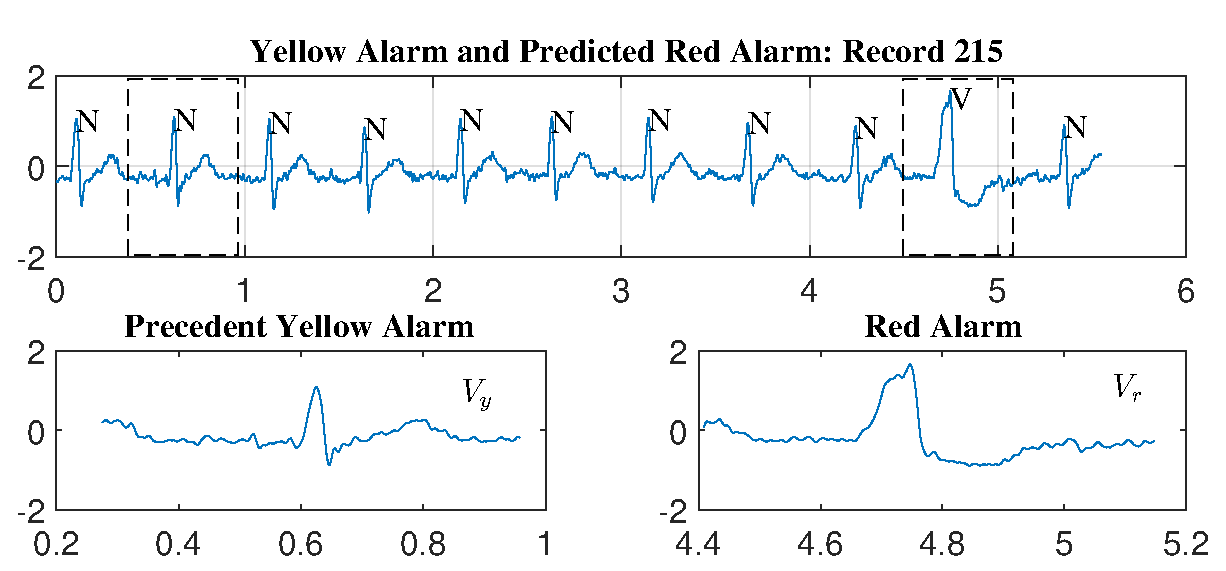
\includegraphics[scale=0.6]{Fig/predicting_record215_croped.pdf} 
 	\caption{Potential latent abnormal status(yellow alarm) predict upcoming abnormality of same type.}
 	\label{fig:pred_signals}
 \end{figure}




\section{Literature Review}
Automatic analysis of ECG signals refers to the entire process from acquisition of signals to classification of samples. This process can be divided into five stages: ECG signal acquisition, preprocessing, fiducial peak detection and segmentation, feature extraction, predictive modeling (Fig. \ref{fig:1-1}). There are researches focus on each single stage in the automatic analysis system. Since the main objectives of this work are addressing problems in classification algorithms, the literature reviews in this section focus on studying existing methods proposed for stages before classification, conventional classification algorithms along with patient-specific classification systems. 

 \begin{figure}[thpb]
 	\centering
 	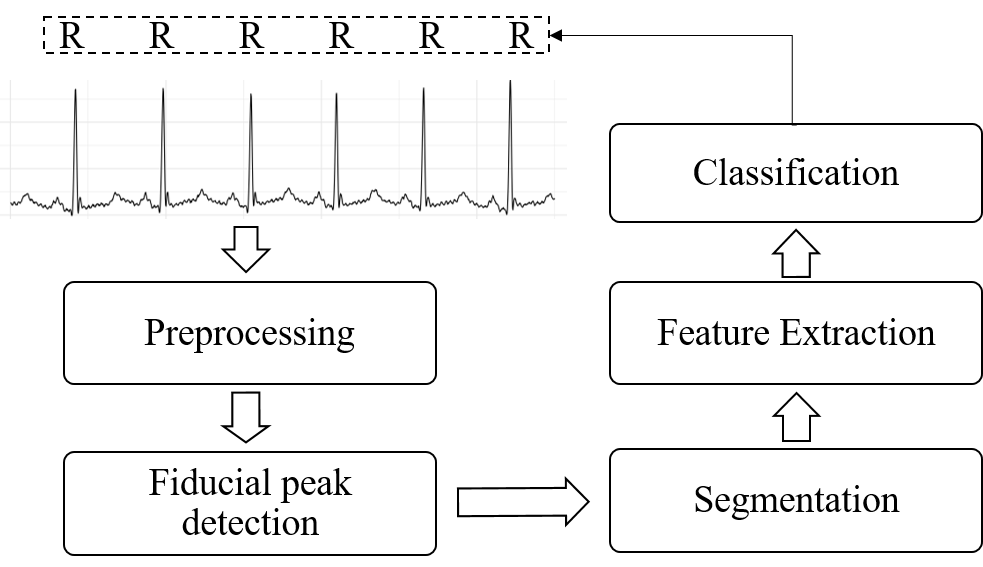
\includegraphics[scale=0.7]{Fig/general_flow.png}  
 	\caption{General structure of ECG classification system}
 	\label{fig:1-1}
 \end{figure}


\subsection{ECG Signal Preprocessing}

During data acquisition, ECG devices often introduce various noises including physiological noises (e.g. myoelectricity noise, breathe interference etc.) and non-physiological noises (e.g. power-frequency interference and electrode impedance interference) \cite{denoise}.These noises often interfere with informative signals and thus influence ECG classification results. Therefore ECG signal preprocessing mainly focus on the suppression of noise interference in ECG signals.

The ECG signal is in millivolt (mV) level with a frequency centered from 0 to 40 Hz\cite{thakor1984estimation}. Since ECG signal is comparatively weak with superposition of various noise, signal preprocessing is necessary step before classification. For this purpose, many researches have been conducted targeting different noise component in ECG signal.

Generally speaking, ECG signal preprocessing methods includes finite impulse response (FIR) filtering,   adaptive filtering, and modern signal processing filter methods such as wavelet transforms and neural networks. Ying -Wen Bai \textit{et al.} compared different notch filters and concluded that equiripple notch filter performs the best on ECG signal. Lian \textit{et al.} \cite{lian2004ecg} designed a multiplier-free finite impulse response (FIR) filters to surpress biological and environmential noises with a low cost of power consumption. Sayadi \textit{et al.} \cite{Sayadi} proposed a modified extended Kalman filter with estimated hidden state variables to perform denoising and compression at the same time. Park \textit{et al.}\cite{21} designed a wavelet adaptive filter to reduce S-T segment distortion due to baseline drift and compared its performance with general adaptive filters. It is found that the wavelet adaptive filtering performance surpasses the general adaptive filters. In \cite{nikolaev2000wavelet}, the authors combined wavelet decomposition with Wiener filtering to filter noise by thresholding which is proved to outperform other thresholding denoising methods. Regarding various wavelet basis function, Singh \textit{et al.} studied the optimal selection of basis function for ECG signal denoising\cite{denoise}. By comparing the classification root mean square error using same classifier and different denoising methods, they concluded that Daubechies filter of order 8 performs the best for ECG classification system.


\subsection{Fiducial Peak Detection and Segmentation}

Fiducial Peak Detection and cardiac cycle segmentation are the basis for extracting important information from ECG signals since a ECG record is usually a continuous time series so the information about single cardiac cycle can only be obtained after segmenting the records. The accuracy and reliability of this stage directly determine the final performance of diagnosis and analysis. 

Fiducial peak detection is also called ECG signal delineation, which aims at localize five characteristic peaks within one cardiac cycle. The most significant peaks are QRS complex consisting of Q, R and S peaks. The other two fiducial peaks are P wave before QRS complex and T wave after QRS complex. As shown in Fig.\ref{fig:fiducial_peaks}, these five characteristic waves along with the onset and offset of QRS complex are often used the depict a cardiac cycle.

 \begin{figure}[thpb]
 	\centering
 	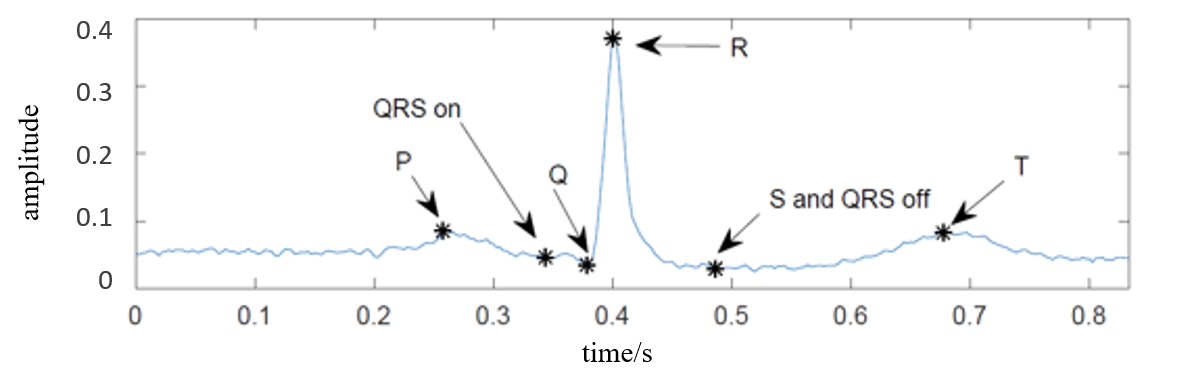
\includegraphics[scale=0.7]{Fig/fiducial_peaks.png}  
 	\caption{Fiducial peaks within one cardiac cycle}
 	\label{fig:fiducial_peaks}
 \end{figure}
 
As QRS complex is the most prominent waves and it contains most of the information of ECG signal, most of the methods for ECG delineation detect QRS complex prior to the detection of other peaks. Afonso \textit{et al.} \cite{afonso1999ecg} proposed a method using filter banks to detect QRS complex. In this method, signal is decomposed to several frequency band. Fiducial peaks are thus detected using its morphological features in the decomposed signals. Sadhukhan \textit{et al.} \cite{sadhukhan2012r} proposed a method of detecting R peak by comparing relative amplitude and double difference. The performance is validated on clinical ECG signal and proved to be promising. Some advanced machine learning techniques are also deployed to detect QRS complex. In \cite{mehta2008svm}, Support Vector Machine is used to train a predictive model for QRS complex detection and achived 99.93\% accuracy. Other pattern recognition models such as Hidden Markov Models are investigated and proved to be effecient in modeling and detecting characteritic peaks in ECG signals\cite{andreao2006ecg}. Wavelet decomposition is also frequently adopted for signal delineation for the morphological similarity between wavelet basis function and QRS complex. As the QRS complex power spectrum is centered at the range of 5 to 30 Hz, wavelet coefficients of corresponding scale levels are frequently used for delineation. In \cite{martinez2004wavelet}, QRS complexes are detected by thresholding wavelet coefficients at scales 1 to 4, then onset, offset and individual waves within QRS complexes are detected using morphological characters of coefficient at scale 2. T and P waves are detected at scale 3 with similar method. Based on this method, some improvements have been proposed to eliminate false detection of R peaks by adding a fixed searching window of 160ms in \cite{banerjee2012delineation}. 

\subsection{Feature Extraction and Classification}

After localize the characteristic point within a cardiac cycle, the classification system needs to extract information in the signal so that the signal could be represented by a set of features. Since the objective of designing automatic classification system is to predict types of sample signal as precise as possible, the feature selection is usually performed to obtain a better performance and reduce the computation cost. 

As the most significant wave within ECG signal, the information within QRS complexes are proved to be the most important features for a ECG classification system. Lagerholm \textit{et al.} decompose QRS complexes with a set of Hermite basis function and the decomposition coefficient are deplyed as ECG features to train the Self-Organizing Map (SOM) which achieved an average error rate of 1.5\% for 16 ECG types\cite{lagerholm2000clustering}. Prasad \textit{et al.}\cite{prasad2003classification} used discrete wavelet transform (DWT) to extract RR intervals between current beat and previous or next beats. The two RR-intervals serves as input for backpropagation neural networks training and the average accuracy of classifying 13 different arrhythmia types is 96.77\%. De Chazal \textit{et al.} proposed two set of features: morphology and heartbeat interval features. They used different combination of these features combined with Linear Discriminant Analysis to classify ECG signal into five arrhythmia types and selected the optimal feature set according to classification performance. The result shows that the sensitivity of detecting two major arrhythmia types can be improved by feature selection. R. Ceylan \textit{et al.}\cite{ceylan2009novel} included RR interval as the only ECG feature to train fuzzy clustering neural network and achieved 98.35\% average detection rate for abnormal samples. Osowski \textit{et al.} adopted High Order Statistics (HOS) and Hermite decomposition coefficients as feature set to classifity ECG signals with Support Vector Machine. Their final average error rate is at 1.82\%\cite{osowski2004support}. %Lannoy \textit{et al.}

\subsection{Patient-Specific ECG Classification}

The main drawbacks of the methods mentioned in the last section is the lack of inter-patient model adjustment. In order to generalize the ECG classification system to clinical application, methods which are more robust to inter-patient signal variation are proposed to address this issue\cite{Hu_et_al,deChazal2006,llamedo2012automatic,bbnn,ince2009generic,Kiranyaz}.

Hu \textit{et al.} proposed a patient-specific mixture of experts (MOE) classifier by incorporating personalized annotations provided cardiologists in the local classifier \cite{Hu_et_al}. This methods achieves patient-adapting capacity but requires further input from human experts. This MOE approach achieved an accuracy of 94.0\% for distinguishing ventricular beats from the other non ventricular types. Following the design of MOE, de Chazal and B. Reilly proposed an improved patient-adapting classifier by reducing the requirement of manual annotations to as few as 10 beats for training adaptive local classifier\cite{deChazal2006}. And Llamedo et al. designed an automatic classification system allowing but not depending on expert assistance\cite{llamedo2012automatic}. By evolving a special block-based neural networks (BbNNs), Jiang et al. achieved accuracies of 98.1\% and 96.6\% for distinguishing ventricular ectopic beats and supraventricular ectopic beats from other types\cite{bbnn}. In \cite{ince2009generic}, particle swarm optimization (PSO) is combined with neural network to optimize network structure using patient specific training data. Based on 1-D convolutional neural networks (CNN), Kiranyaz et al. proposed a flexible algorithm which adjusts its parameters using information extracted from individual signal\cite{Kiranyaz}. The classifier demonstrates consistent performance over different ECG records achieving an accuracy between 98\% ~ 99\% for distinguishing VEBs from non-VEBs. (Acc = 98.9\%  Sen = 95.9\% Spe =  99.4\%). While this approach outperforms the aforementioned classification algorithms as it does not require expert further annotations, its performance reduces for some rare abnormal classes. 
 
\section{Contributions}

A crucial drawback of these patient-specific classification systems in the literature are their deficiency of predicting abnormality in advance. Conventionally, classifiers associate each sample with a label and optimize performance according to the uniformity of proposed label and ground truth. While in many common applications this concept drives satisfying results, it does not meet the needs of SCD prediction. %Combining patient-specific classifier and the character of ECG signal analysis, we proposed a patient-adaptable classification framework with a nonlinear transformation module to assist quantifying latent status between normal and abnormal types.

One of the main objective of this work is to address the problem of forecasting by proposing two different feature space transformations to optimize the predicting capacity of personalized classifier for applications using biomedical signals. To specify this scenario, we assume that there are one normal status and multiple abnormal status for a signal while latent status exists for normalities with deviation towards abnormalities, indicating information regarding subsequent abnormalities. By distinguishing  latent status, the designed automated system is capable to generate yellow alarms which indicates a high probability of proceeding presence of same type abnormalities. Therefore the contribution of this work can be summarized as:

\begin{itemize}
    \item Proposed a novel self-adapting patient-adaptable framework  which incorporate a personal classifier enabling predictive modeling
    \item Studied kernel-based method as spatial transformation with parameters optimized with Multi-Objective Particle Swarm Optimization for the purpose of deviation quantification
    \item Designed a controlled spatial transformation with deterministic mapping function to optimize cluster topology for predictive analysis
    \item Proposed a deviation quantification method based on cosine similarities which is able to generate predicting alarms for upcoming abnormalities
\end{itemize}


\section{Organization of Thesis}

In the following chapters, details of proposed classification frameworks are introduced along with the background of algorithms deployed in the framework. To start with chapter 2 provides a general introduction to the dataset used in this thesis and the general frameworks of the proposed classification system. Following this framework, chapter 3 further described the details of nonlinear transformation with kernel methods and presented the experimental results using kernel transformation. With the concept of nonlinear transformation, chapter 4 introduced an optimized spatial transformation method with a novel deterministic mapping function. The experimental result of the spatial transformation method is presented and studied in section \ref{sec:result_spatial}. Finally, the experimental results of the methods proposed in chapter 4 and chapter 5 are compared. More importantly, the predicting capacity of systems are studied and analyzed. Based on the experimental results, we analyzed the potential future works in order to further optimize the system in both classification and predicting accuracy.

%\chapter{Patient-Adaptable ECG Classification Framework}

\section{Introduction}
For decades, automatic ECG signal analysis has been a controversial research topic. Several academic research projects have proved that the design and implementation of automatic ECG analysis methods is beneficial for timely detection and therapeutic intervention of heart diseases. However, some major challenges should to be resolved, and automatic ECG analysis should reach a level of maturity and reliability before getting ready for clinical use. One of the most typical challenges is the inherent inter-patient variation of ECG waveforms, which leads to inconsistent performance of ECG classification systems when applied to different patients under different conditions. In this chapter, the details of the patient-adaptable ECG classification method, as the core of the proposed framework are presented.

The goal of automatic ECG analysis is to determine the arrhythmia types for each signal sample. Continuous ECG signal is firstly segmented into individual intervals, each of which represents a heartbeat cycle, to be processed by the further stages of the proposed algorithm. \textcolor{black}{Section 2.2 and Section 2.3} in this chapter focus on the data preparation stage, which includes four steps: signal preprocessing, delineation, segmentation, and feature extraction. Following the data preparation, \textcolor{black{Section 2.4} elaborates on the details of the proposed two-stage hierarchical classifier. The proposed classification system introduces a novel method for patient-adaptation by gradually capturing the normal range for each individual. More specifically, in Section 2.4, the dynamic normal cluster shaping method to achieve rationalization property is discussed. One feature of this method is that the cluster can track a patient's ECG waveform changes and dynamically adapt to it. In many applications, the physicians need to monitor a long-term real-time heart activity. This dynamic adaptation is able to address the issue of intra-patient temporal signal variation as well.

%In many application scenarios, the method of manual analysis is too complicated and time-consuming to implement. In addition, automatic electrocardiogram analysis has a very important role in monitoring long-term real-time heart activity, because manual monitoring and interpretation are not feasible under these application scenarios. It can be seen that the development of a reliable automatic heartbeat classification algorithm will be conducive to the diagnosis of arrhythmia, so this study will focus on this issue.

%The main goal of this chapter is to introduce the basic framework of automatic heartbeat classification, including ECG signal processing, characterization and classification. The rest of this chapter is organized as follows: Section 2.2 elaborated on the first step of ECG analysis, namely the preprocessing of ECG signals, including filtering and denoising; Section 2.3 immediately follows the previous section, and described the detection methods and periodic segmentation methods for the various peaks in the cardiac cycle. In particular, the multi-stroke segmentation method used in the algorithm described in this article was explained in detail; Section 2.4 introduced the steps of feature extraction and the feature quantities used in this paper based on the segmentation method used in this algorithm. The last section 2.5 is a summary of the contents of this chapter. The author reduced all the steps before the classification algorithm to a mapping and briefly outlined the structure of the classification algorithm.

\section{ECG Signal Processing}

\subsection{Preprocessing}
Biomedical signals, such as ECG signals, composed of a sequence of signal segments, that can be presented by a set of statistical, morphological, and spectral features. Since the signal properties change over time, the traditional Fourier transform is not suitable for this type of non-stationary signals since it is unable to capture time-varying statistics of the signal. Wavelet decomposition solves this problem by scaling and translating mother wavelet to constitute its basis functions, which capture both spectral and temporal properties of the signal. Given a time series, wavelet decomposition decomposes the signal into linear combinations of basis functions. Thus, basis functions with larger scales are smoother than those with smaller scales and consequently correspond to lower frequency components of the signal. Similarly, the coefficients of the decomposition correspond to higher frequencies when the scale is smaller. Using wavelet decomposition, we extract both time and frequency features of the signal.

%\textcolor{red}{Here} 

In this work, wavelet analysis is applied to ECG signals in MITDB with a sampling frequency of 360 Hz. Daubechies wavelet of order 8 ($db8$) is selected as mother wavelet for denoising stage in this work for its optimal performance\cite{denoise}. The decomposition coefficients and their corresponding frequency components are presented in Fig.\ref{fig:wavelet_decomp}. \textcolor{red}{Consistently use Fig. or Figure without dot "." throughout the thesis.}

Low frequency noise or baseline wander between 0.15 to 1 Hz, caused by respiration and body movement, can be removed by deducting the approximation coefficient of level 8 ($A_8$) from the signal. Since the power of ECG signal is mainly concentrated in the frequency band from 1 to 40 Hz, higher frequency terms are more likely to represent noise terms including electromyogram induced noise and mechanical forces acting on the electrodes. These terms can be removed by discarding the detail coefficient of level 1 ($D_1$). 

\subsection{Segmentation}

Most machine learning (ML) algorithms operate on input vectors and are not directly applicable to continuous-signals. Therefore, biomedical signals are typically converted to a representative vector before incorporating to ML algorithms. We follow the common trend of translating a signal segment into a vector of representative features. In this regard, we first need to split the signal in time domain into smaller segments. To obtain more relevant results, we choose the segments as one or multiple consecutive cardiac samples, noting the fact that each cardiac cycles is associated with a label based on experts observation. 

Most existing methods use wavelet analysis to detect the highest peak (R wave) in a cardiac cycle as a reference point and then use signal morphology and typical properties of other waves to determine boundaries between consecutive intervals \textcolor{blue}{[REF]}. In this study, we use this common approach. As was earlier mentioned in Section \ref{sec:fiducial_peaks}, a cardiac cycle consists of five basic characteristic peaks: P, Q, R, S, and T. Among them, the QRS complex is the most significant peak in one cycle. The energy of ECG signal in one cardiac cycle is mainly concentrated within the QRS complex. The QRS complex also conveys important information that reflects the arrhythmia category\cite{2012qrs}. Accurate detection of the QRS complex is of crucial importance for subsequent analysis. The energy of the QRS complex is generally within the range of 5-25 Hz. For ECG signals with sampling frequency of 360Hz, the QRS complex can be extracted from the detail coefficients of level 5 ($D_5$) and level 6 ($D_6$)

\begin{figure}[t]
\centering
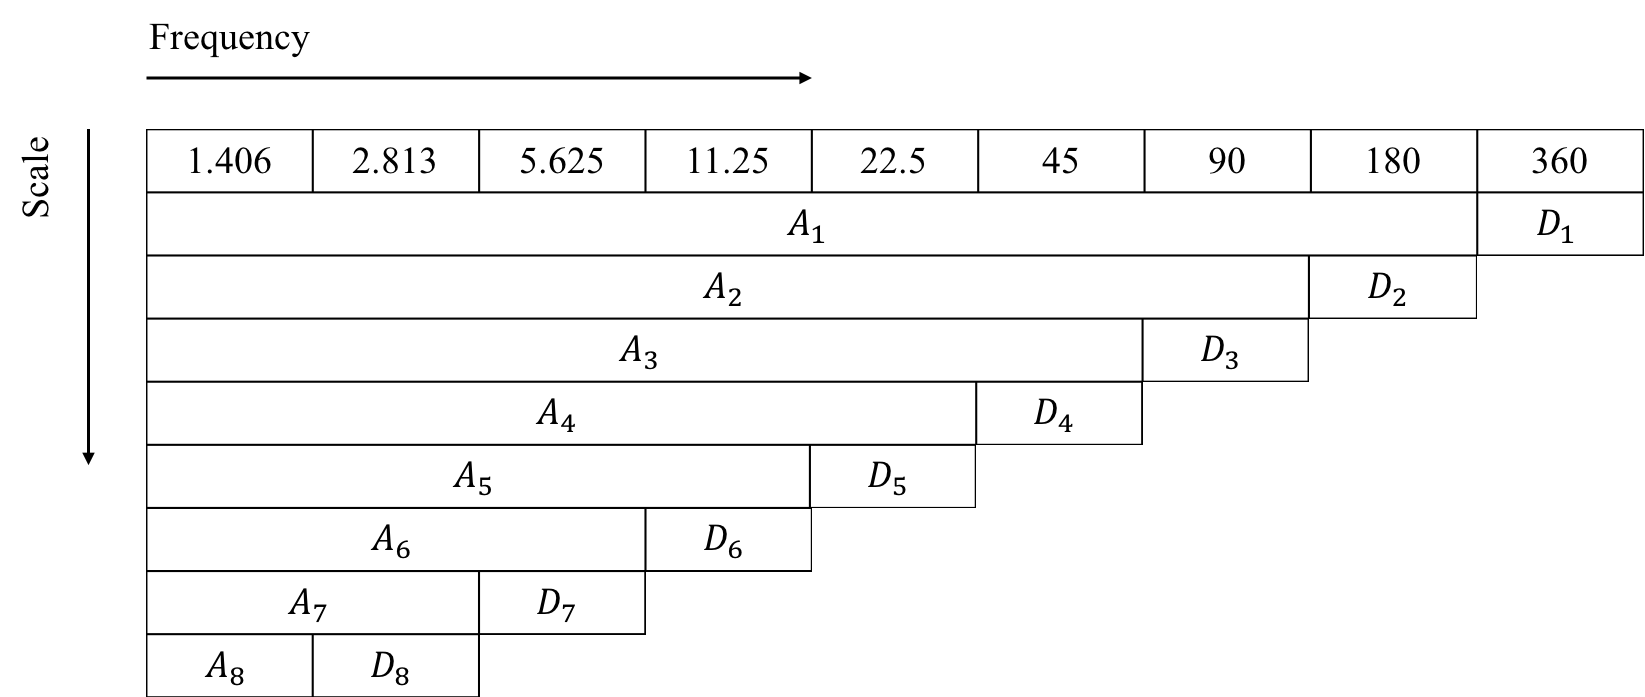
\includegraphics[scale=.5]{Fig/scale_wavelet.png}
\caption{Frequency band of wavelet decomposition coefficients for MITDB signals}
\label{fig:wavelet_decomp}
\end{figure}


The mother wavelet $db4$ is utilized at this stage due to its morphological similarity to QRS complexes. By superimposing $D_5$ and $D_6$, the QRS complex information in the ECG signal can be characterized in a one-dimensional recombined signal ($QRS\_DET = D_5+D_6$).Other Fiducial peaks (P, QRS onset, Q, S, QRS offset and T waves for each cardiac circle) are localized according to an algorithm proposed in \cite{2012qrs}. The accuracy of peak detection and its coincidence with the true signal is shown in Fig.\ref{fig:QRS_d5d6}.

\begin{figure}[t]
\centering
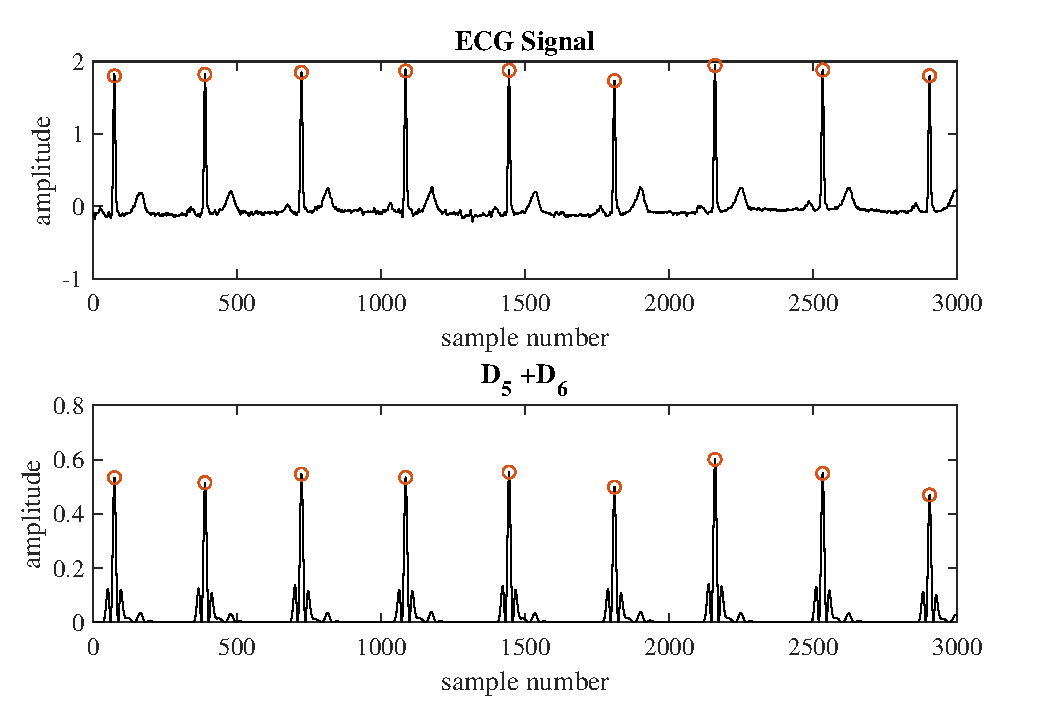
\includegraphics[scale=.7]{Fig/QRS_D5D6.pdf}
\caption{QRS detection with wavelet coefficients of level 5 and level 6. \textcolor{red}{Add dot to all captions. Also, it is good to use subfigure with captions (a) and (b) and then include the full description in the caption.}}
\label{fig:QRS_d5d6}
\end{figure}


With the empirical values described in \cite{2012qrs}, we use 15\% as the detection threshold. Since the width of most of the QRS complexes does not exceed 160ms, here we use a sliding window with a width of 160ms to detect the peaks in the $QRS\_DET$. The window step size is set to 200ms, given that the time lag between the two adjacent heartbeat cycles does not exceed 200ms.  Figure.\ref{fig:window} shows a typical $QRS\_DET$ waveform along with the corresponding window of width 160ms. The false peaks are eliminated using a 160ms time window, as seen in Figure.\ref{fig:window}.


\begin{figure}[t]
\centering
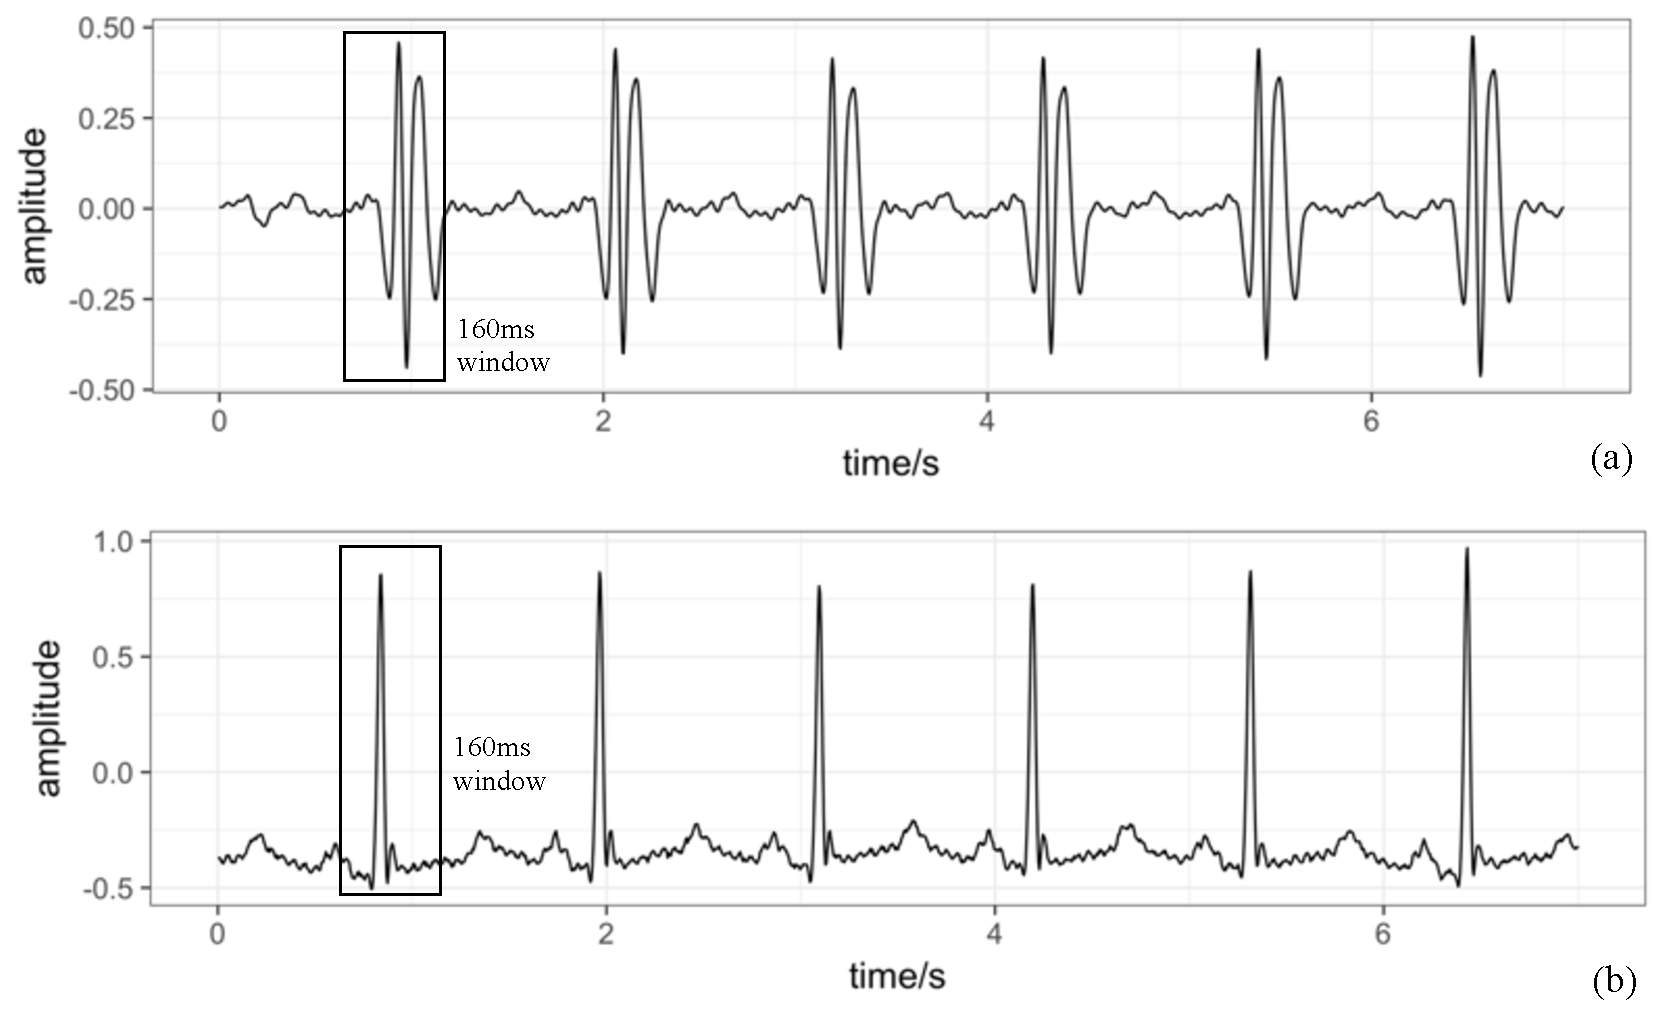
\includegraphics[scale=.5]{Fig/window.pdf}
\caption{Window for detecting R peaks within QRS complexes}
\label{fig:window}
\end{figure}


The T and P waves are outside the QRS window. Through scanning the region spanning the start of a QRS window to the end of its neighboring QRS \textcolor{red}{I think you mean: the end of a cardiac interval to the beginning of QRS window in the next interval}, the P-wave is located as the highest positive peak in this region. In a similar way, the position of the T wave is obtained by finding the maximum of the signal in the region between the from the end of the QRS in the current cardiac interval to the beginning of the next cardiac interval. \textcolor{blue}{In an alternative way, the two peaks between the two consecutive QRS windows, respectively represent the T and P waves.}
In short, an ECG signal in one heartbeat segment can be fully described by 7 feature points: P, QRS on, Q, R, S, QRS off and T. 

After localizing the feature points, we can use the location of R peaks to determine the boundaries of a cardiac cycle. %Wwave, a segment of the ECG signal was divided into cardiac cycles. 
By processing a large number of ECG signals, we realize that R peaks approximately split cardiac cycles into two pieces with $1/3$ and $2/3$ of the entire signal. \textcolor{red}{Add REF if any}. 
Based on this observation in the morphology of a typical ECG signal, we define the starting point of a cardiac cycle as the point which divides the distance between the two consecutive R waves into two sections, where the length of the first section is half the length of the second section, as depicted in Fig. {fig:interval}. In this figure, the distance (RR) between the two adjacent R waves is denoted by $h$, therefore R wave is located in distance $h/3$ with respect to the beginning of the cycle. The advantage of this method is its low computational complexity and easy generalization to different patients, noting that a slight change in cardiac boundaries do not significantly alter the properties of a cardiac cycle as long T and P waives remain in the correct interval. 

The quality of ECG signals provided by most of the portable ECG measuring instruments is very unstable and may include transient noises. Signals transmitted through wireless communication systems will exhibit even more unstable waveforms. These transient effects appear in the resulting feature vector and consequently they negatively affect the prediction accuracy of the subsequent ML method. In order to eliminate and smooth out these transient terms, we use the concept f \textit{segmentation} here, where each segment includes multiple cardiac intervals, 
%Moreover, the objective of this work is predictive modeling, thus by including statistical features capturing change between consecutive beats, the system obtains information regarding the following beats. Taking these facts into account, this work performed subsequent feature extraction and analysis combined three consecutive cardiac cycles (i.e. one representative segment). In the subsequent analysis, an segment is considered as a sample of data 
as shown in Fig.~\ref{fig:interval}. \textcolor{blue}{Note that the number of cycles in each segment is a modeling parameter shown by $XXX$. Also, we can arbitrarily slide segments equivalent to $YYY$ cycles to generate the new feature vector. The parameters $XXX$ and $YYY$ can be tuned to improve the overall performance of the method.  Based on intensive simulations, we choose $XXX=xxx$ and $YYY=yyy$, which yield the best classification accuracy. In Fig.~\ref{fig:interval}, we have $XXX=xxx$ and $YYY=yyy$.}

\begin{figure}[t]
\centering
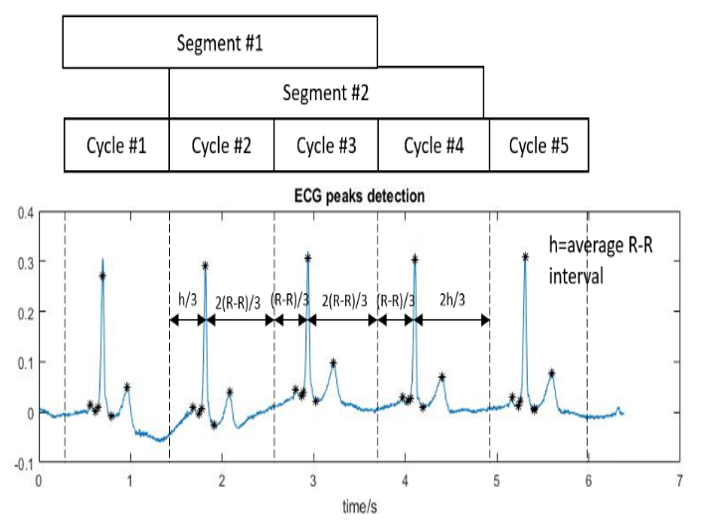
\includegraphics[scale=.8]{Fig/segment.png}
\caption{Segment samples correspond to three consecutive cardiac cycles}
\label{fig:interval}
\end{figure}


\textcolor{red}{This is not well connected to the text before and after. Make it a separate Section titled as 2.2 Utilized Dataset and move it to the beginning of this section.}
%\subsection{Dataset}
For the purpose of training and evaluating classifier, MITDB is split into test (DS2) and training (DS1) set by balancing the four classes according to \cite{autofs}. 



The ECG signals in MITDB dataset are annotated and labels are provided for each cycle. However, we define a segment, which may include more than one sample as a sample. Therefore, we need to translate per-cycle labels into per-segment samples. In this regard, a new label for each segment is generated by integrating all annotations of the beats within the segment. The segmend is labeled as \textit{normal}, if all member beats are annotated as N; otherwise, this segment will be labeled as the abnormality type of its member beats if there is only one abnormality type. If more than one abnormality types are present within the same segment, the segment is excluded. \textcolor{blue}{For instance, segments with members labels "NNN", "SSS", "NVV", "VVV" are respectively mapped to "N","S", "V", and "V", and a segment with member label "NVS" is discarded.} 
After segmentation and new annotation, the total number of samples in the training and test set are obtained as summarized in Table.\ref{table:ds}
\begin{table}[b]
	\centering
	\caption{Training and test datasets in MITDB.}
	\vspace{-0.05in}
	\begin{tabular}{|l||c|c|c|c|c|}
		\hline 
		& \multicolumn{4}{c}{Number of segments per AAMI class} &\\ 
		\hline 
		Evaluation Dataset& N & V & S & F &Total \\ 
		\hline 
		DS1:Training & 11721& 2356 & 862 & 256 & 15195\\ 
		\hline 
		DS2:Test & 12633 & 2053 & 550 & 121 & 15357 \\ 
		\hline 
		Total & 24354 & 4409 & 1412 & 377 & 30552 \\ 
		\hline 
	\end{tabular}
	\label{table:ds} 
	\vspace{-0.15in}
\end{table}

\section{Feature Extraction}

The feature extraction step plays a crucial role in the diagnosis of heart disease and has a great influence on the performance of the subsequent automated classification systems. De Chazal et al. have studied the impact of using waveform morphological features on classification results \cite{autofs}. As discussed in \cite{jambukia2015classification}, the combination of three types of characteristics (i.e. temporal, morphology, and frequency domain features) can provide a better discriminative power for the classification algorithm to distinguish between different types of arrhythmia. 

According to several studies different types of ECG signals mainly differ in the power level of the frequency band ranging from 5 Hz to 15 Hz \cite{XXX}. Likewise, some other morphological features (such as the duration between the Q wave and the T wave, P The distance to the R wave, etc.) present different levels of correlation with a specific signal classes \cite{XXX}. Therefore, we choose to use combination of temporal, morphological and spectral features as detailed in Table \ref{table:features}. Also, to account for segment-level characteristics as well as cycle-level properties, the extracted features include both periodic-based features (SET 1) and segment-based features (SET 2), where SET1 includes the average and standard deviation of the corresponding features of the three cardiac cycles within a segment, and SET2 contains the overall characteristics of the time signal within the segment, so it is calculated only once per segment. Therefore, we have a total of \textcolor{blue}{$8 \times 2 + 6 =22$} features per segment as shown in Table \ref{table:features}. Therefore, each feature vector is a $22×1$ vector with zero-mean unit-variance elements after a proper normalization. %Summarized details are described in Table.\ref{table:features}.
In Table~.\ref{table:features}, mean $(R_{i+1}-R_i)$ refers to the mean of the time lag between two adjacent R waves, while $(R_i-R_{avg})$ is the length of each cardiac cycle and the average cardiac cycle duration of the patient. 

\begin{table}[t]
	\caption{Features extracted from ECG signal\textcolor{red}{. Change column width such that each line represents one feature.}}
	\label{table:features}
	\centering
	%\begin{flushleft}
	\begin{tabular}{|m{6em} || @{}m{7.4em} ||@{} m{7.7em}|}
		\hline 
		Feature Type & SET1 & SET2 \\ 
		\hline 
		Temporal Features & QRS duration, ~~~~
		QT duration, ~~~~~~~
		PR duration & mean$(R_{i+1}-R_i)$, mean$(R_i-R_{avg})$  \\ 
		\hline 
		Morphological Features & max positive peak to second peak ratio & signal average energy, max positive peak, max
		negative
		peak, peak to
		energy ratio \\ 
		\hline 
		Frequency Domain Features & signal power level at 7.5Hz, 10Hz, 12.5Hz, 15Hz &  \\ 
		\hline 
	\end{tabular} 
	%\end{flushleft}
\end{table}

From Table.\ref{table:features}, one may notice that these 22 feature are not completely independent of each other. Also, some of the features may not be as relevant as the others. Therefore, we reduce the number of features to obtain a more robust predictive modeling \cite{Some references for feature selection}. We use Principal Component Analysis (PCA) \textcolor{red}{or principal component analysis (PCA): choose one notation} as a commonly used the common dimension reduction method instead of explicit feature selection for its improved performance in biomedical signal processing \cite{Some references for PCA as a dimension reduction method}. We keep the 8 dominant directions of the signal after PCA as the most informative 8 features.



\section{Classification Framework}

\textcolor{red}{part of the following text is related to global classifier, and part of it to deviation analysis (including personalized normal cluster, ...). Use subsections as needed to be more clear.}

In this section, we elaborate on the details of the proposed methodoology to perform the classification and prediction tasks using the pre-processed ECG data. Based on our previous study \cite{chen2018predictive} as well as similar prioir works on developing patient-specific classifiers \cite{Hu_et_al,deChazal2006,llamedo2012automatic}, we propose a two-staged structure which includes a global classifier to capture general properties of different classes followed by a personalized classifier to capture patient-specific properties~\cite{chen2018predictive,Hu_et_al,deChazal2006,llamedo2012automatic}. Moreover, the proposed algorithm incorporates a novel deviation analysis module with details presented in the following sections. 


The flowchart in Figure \ref{fig:flow} presents the overall operation of the proposed system. The \textit{global classifier} is trained using the whole training dataset as the first classification step. It facilitates the subsequent analysis in the system by identifying samples with severe morbidity. Depending on the application (properties of signals, the utilized labels, and the choice of features), different classification algorithms can be utilized \cite{REF}. Two important considerations include the classification accuracy and the computation complexity of the method \cite{REF}. Any abnormal label generated by the global classifier is considered as a \textit{red alarm} and does not require further processing. However, samples labeled as  \textit{normal} go through the subsequent personalized classification step. 

\begin{figure}[ht]
	\centering
	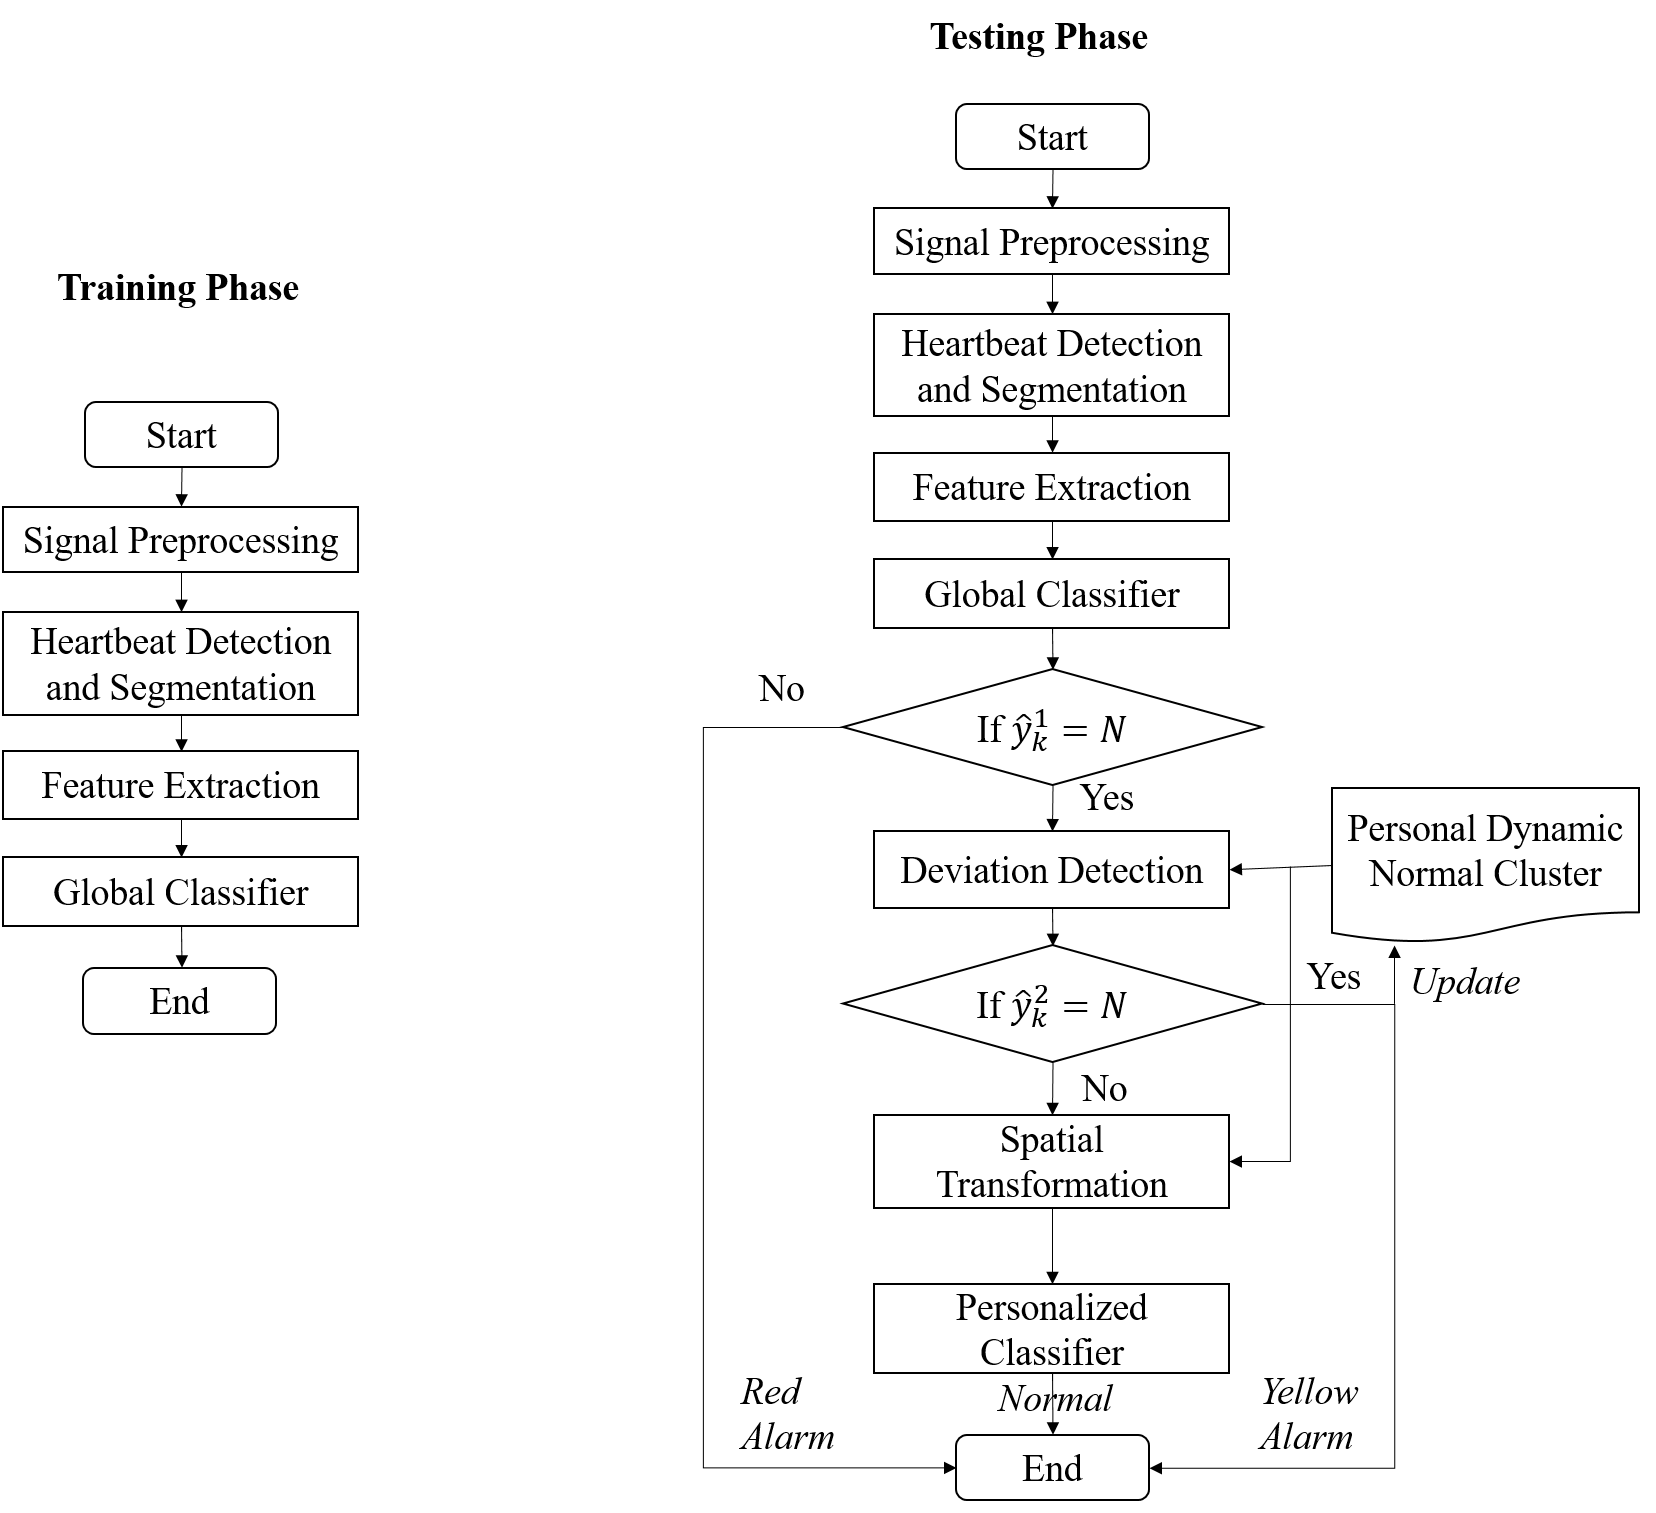
\includegraphics[scale=.5]{Fig/flow2.png}
	\caption{The general flowchart of proposed framework}
	\label{fig:flow}
\end{figure}





Since, one objective of this study is to identify the fuzzy states between normality and abnormalities, the subsequent analysis is focused on processing samples classified as \textit{normal}(N) \textcolor{red}{use a consistent notation: you can choose to use italic font for ``normal'' and ``abnormal'', ``red'', ``yellow'', etc in their first appearance or for all appearances.  Also, define labels N, S, ... on their first appearances.} to check whether or not they show considerable deviations to one of the abnormality classes. For this purpose, a one-layer classifier is not sufficient \textcolor{blue}{due to multiple reasons: i) the numbers of samples in the normal and different morbid classes are not balanced in the training set DS1 as shown in Table.\ref{table:ds}, ii) the patient-specific normal trend is not known, iii) determining yellow alarms require a new set of decision rules to determine whether or not the deviations are worthy of calling a yellow alarm.} Therefore, a deviation detection module is added after the Global Classifier to identify \textcolor{red}{latent has a special meaning in ML, which is different than what you mean., I recommend change ``latent'' to a different word} %latent status 
yellow alarms using patient-specific normal cluster. In order to develop a ground for patient-specific normal functionality and adapt the classifier accordingly, the first 20\% of total Normal samples of each patient are selected as the initialization of \textit{personalized dynamic normal cluster} $\mathcal{N}_0^k$. To do this, we use a binary classification of N versus non-N, where the second includes all abnormal classes. We firstly calculate the following distance metrics:

\begin{align}
\label{eq:matrices}
R_i^{\max}=\underset{\mathbf{x}_j\in\mathcal{N}_i^k,\mathbf{x}_k\in\mathcal{N}_i^k}{\max}\{\sqrt{(\mathbf{x}_j-\mathbf{x}_k)^2}\},
\\
D_\mathcal{X}(\mathbf{x}_k(i))=\underset{\mathbf{x} \in\mathcal{X}}{\text{median}}\{\sqrt{(\mathbf{x}_k(i)-\mathbf{x})^2}\},
\\
D_\mathcal{N}^{\max}(\mathbf{x}_k(i))=\underset{\mathbf{x} \in\mathcal{N}_i^k}{\text{max}}\{\sqrt{(\mathbf{x}_k(i)-\mathbf{x})^2}\},
%D_V(x^t)=\underset{x_V\in\Omega_V}{\text{median}}\{\sqrt{(x^t-x_V)^2}\}\\
%D_S(x^t)=\underset{x_S\in\Omega_S}{\text{median}}\{\sqrt{(x^t-x_S)^2}\}\\
%D_F(x^t)=\underset{x_N\in\Omega_F}{\text{median}}\{\sqrt{(x^t-x_F)^2}\}\\
%D_{max}(x^t)=\underset{x_N\in\Omega_N^t}{\max}\{\sqrt{(x^t-x_N)^2}\}
\end{align}

The following conditions are then examined to verify if the deviation of a sample is within the range defined by $\alpha$. Since some rare abnormalities are unlikely to be observed within the limited initialization period, therefore abnormal clusters: ${\mathcal{S},\mathcal{V},\mathcal{F}}$, which include abnormal beats for all patients in DS1, are deployed as the training dataset when developing the  \textit{personalized dynamic normal cluster} $\mathcal{N}_i^k$ as follows. \textcolor{red}{I think here in $\mathcal{N}_i^k$, you mean that $i=0$ represents the normal cluster and $i=1,2,...$ represent different abnormality clusters. This is not obvious and you need define it before its first appearance.}

\begin{align}\label{eq:condition1}
\begin{cases}
D_\mathcal{N}^{\max}(\mathbf{x}_k(i))  \leq\alpha R_i^{\max},\\
D_\mathcal{N}(\mathbf{x}_k(i)) < D_\mathcal{X}(\mathbf{x}_k(i)) &\text{for~} \mathcal{X}\in\{\mathcal{S},\mathcal{V},\mathcal{F}\}   %(D_N(x^t),D_V(x^t),D_S(x^t),D_F(x^t))=D_N(x^t)
\end{cases}
\end{align}

If a sample already called normal by the global classifier, is again confirmed as N in this module, it will be used to update the $\mathcal{N}_i^k$. Otherwise, the system assumes that the sample has a considerable deviation towards one of the abnormal clusters and hence will pass it to the subsequent \textcolor{blue}{\textit{personalized classifier}}. The \textit{personalized classifier} uses controlled transformation with optimized parameters to discern the deviation to different morbid types regardless of the cluster topology within the original feature space \textcolor{blue}{, as detailed in Section XXX}. 

After performing both global and personalized classification steps, a given sample $x_k$ at time $k$ is mapped to label $\hat{y}_k \in \{N,Y_V,Y_S,Y_F,R_V,R_S,R_F\}$, where $N$ stands for normal status, $Y_X$ stands for a ventricular yellow alarm of type ``X'', and $R_X$ stands for a ventricular red alarm of type ``X''.

\begin{figure}[t]
\centering
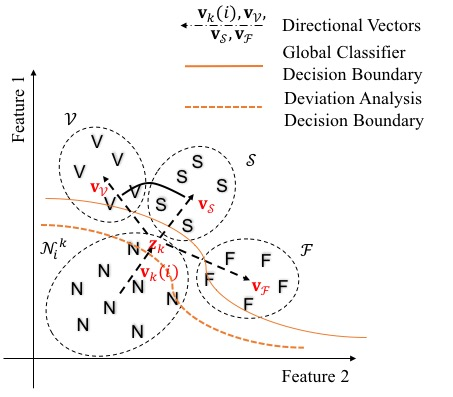
\includegraphics[scale=.7]{Fig/topology.jpg}
\caption{The deviation analysis boundary restrict on latent status between normal and abnormal samples compared with the Global Classifier boundary}
\label{fig:topo_deviation}
\end{figure}


\section{Personal Classifier} \textcolor{red}{I suggest you use the term personalized classifier, although personal classifier is correct too.}

Here, we provide the core idea behind the design of the personalized classifier, and the details of implementation will be discussed in \textcolor{blue}{Chapters 3 and 4.} 
Since the proposed system aims at predicting subsequent abnormalities by analyzing a signal's deviation from the patient's normal functionality of the sample signal, it is vital to quantify the deviations using topological characteristics of the training dataset. For most of the ECG applications, ECG signal is analyzed by its representative feature vectors. A natural choice for deviation analysis in the high-dimensional feature space, is Cosine Distance \textcolor{blue}{\textit{cosine distance}} as defined in Eq.\ref{eq:cosine}) to quantify the distance between two vectors $\textbf{v}$ and $\textbf{w}$.

\begin{align}
\label{eq:cosine}
d(\mathbf{v},\mathbf{w})= 1 - \frac{\mathbf{v}^T\mathbf{w}}{|\mathbf{v}||\mathbf{w}|}=1 - \frac{\mathbf{v}^T\mathbf{w}}{\sqrt{(\mathbf{v}^T\mathbf{v})(\mathbf{w}^T\mathbf{w})}}
\end{align}

Consequently, relative deviations of a sample from normal cluster(N) to other abnormal clusters (V, S, F) are defined by the cosine distance between the vector $\mathbf{v}_k(i)$ (defined in Eq.\ref{eq:v_k}) and the three vectors $\mathbf{v}_{\mathcal{X}}(i)=\mathbf{c}_{\mathcal{X}}-\mathbf{x}_k(i)$ where $\mathcal{X} \in \{ \mathcal{S}, \mathcal{V}, \mathcal{F}\}$. \textcolor{blue}{In this case, a smaller cosine distance represents a higher alignment between the vector from the normal cluster centroid $\mathbf{v}_k(i)$ to the current sample $\mathbf{x}_k(i)$ and the reference vector from the normal cluster centroid to abnormal centroids $\mathbf{c}_{\mathcal{X}}$.}


\begin{align}
\label{eq:v_k}
%\mathbf{v}_k=\mathbf{x}_k-\mathbf{c}_N^k = \mathbf{x}_k- \frac{\sum_{j=1}^{k-1} \mathbf{x}_j I(\hat{y}_j=N)}{\sum_{j=1}^{k-1}  I(\hat{y}_j=N)}, 
\mathbf{v}_k(i)=\mathbf{x}_k(i)-\mathbf{c}_N^k(i) = \mathbf{x}_k(i)- {\sum_{\mathbf{x} \in \mathcal{N}_i^k} \mathbf{x}}/{|\mathcal{N}_i^k|}, 
\end{align}

Therefore, the classification result of the Personal Classifier $\hat{y}^2_k(i)$ is determined as follows:

\begin{align}
\label{eq:personal_discrim}
\hat{y}^2_k(i) = \underset{\mathcal{X} \in \{ \mathcal{S}, \mathcal{V}, \mathcal{F} \}}{\text{argmin}}\{ d(\mathbf{v}_k(i),\mathbf{v}_{\mathcal{X}}(i)) \} 
\end{align}

The relevance of cosine distance depend on the topology of clusters in the feature space. The topology in feature space, itself is inherited from the feature extraction and feature selection methods. For example, as shown in Fig.\ref{fig:topo1}, in the original feature space overlaps and alignment of abnormal clusters may lead to inaccurate results of deviation quantification. \textcolor{blue}{In order to eliminate the deviation analysis errors that arise from the asymmetry in the clustering topology, it is desired to transform the original topology into a more symmetric topology, where cosine distances directly reflect the amount of deviations.}

\begin{figure}[thpb]
\centering
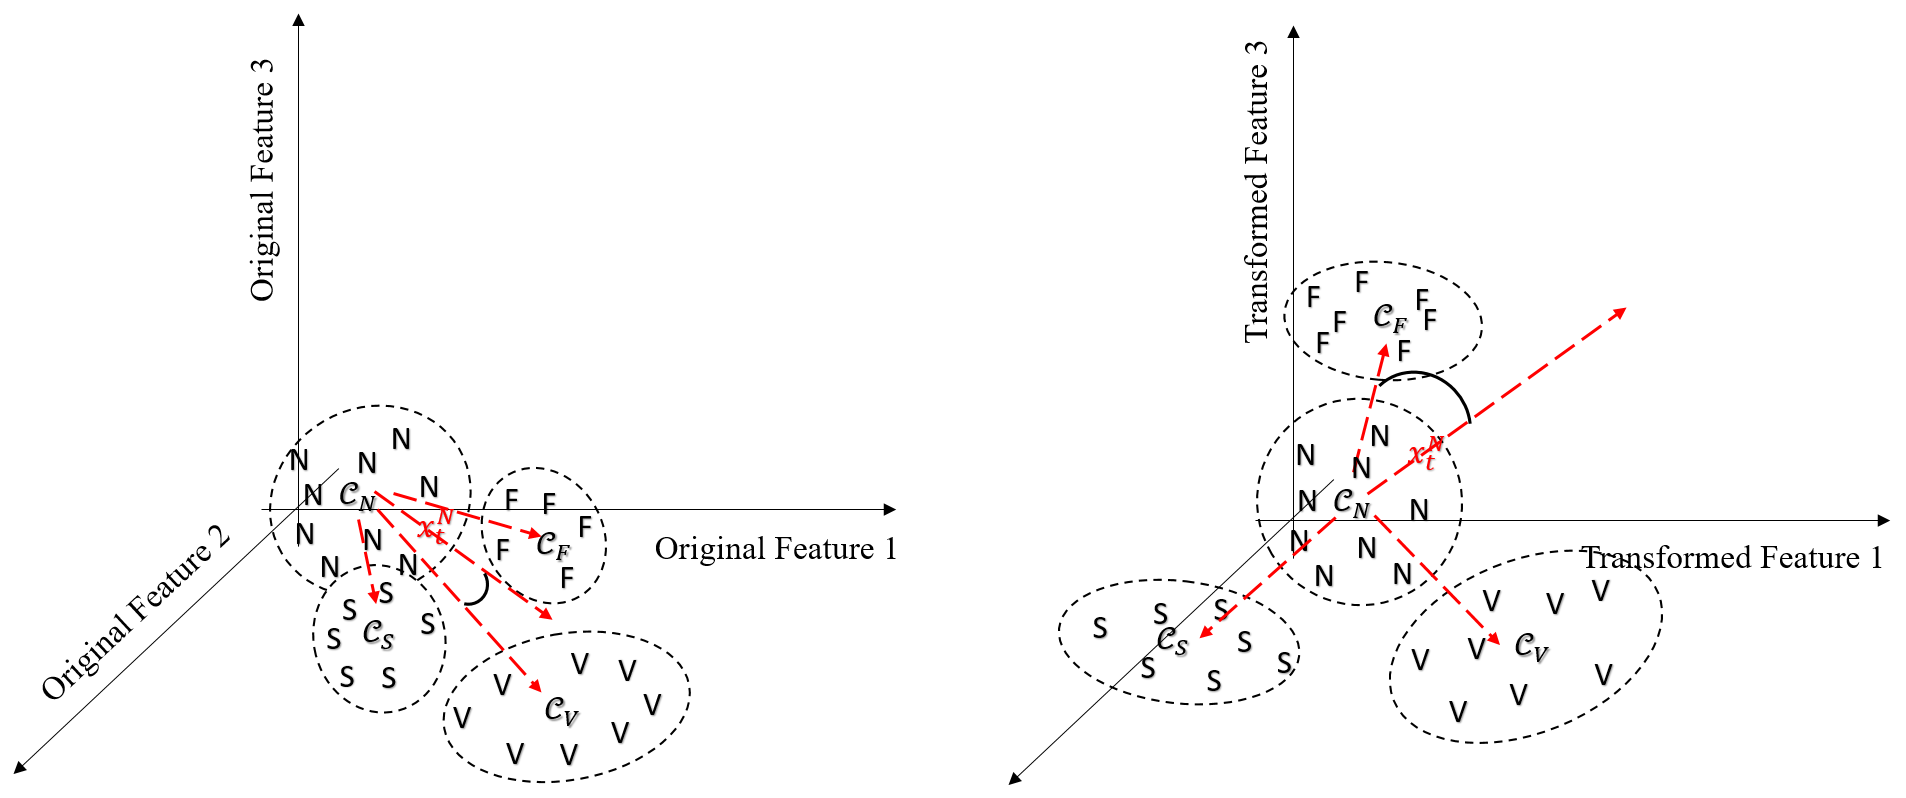
\includegraphics[scale=.5]{Fig/topo1.png}
\caption{Left: illustration of the cluster topology in the original feature space; Right: illustration of the cluster topology in the transformed feature space using a nonlinear mapping function.}
\label{fig:topo1}
\end{figure}

For this purpose, two different spatial transformation methods are proposed in the next two chapters.

%\chapter{Patient-Adaptable ECG Classification Framework}

\section{Introduction}
For decades, automatic ECG signal analysis has been a controversial research topic. Several academic research projects have proved that the design and implementation of automatic ECG analysis methods is beneficial for timely detection and therapeutic intervention of heart diseases. However, some major challenges should to be resolved, and automatic ECG analysis should reach a level of maturity and reliability before getting ready for clinical use. One of the most typical challenges is the inherent inter-patient variation of ECG waveforms, which leads to inconsistent performance of ECG classification systems when applied to different patients under different conditions. In this chapter, the details of the patient-adaptable ECG classification method, as the core of the proposed framework are presented.

The goal of automatic ECG analysis is to determine the arrhythmia types for each signal sample. Continuous ECG signal is firstly segmented into individual segments, each of which represents a heartbeat cycle, to be processed by the further stages of the proposed algorithm. \textcolor{blue}{Section 2.1} in this chapter focuses on the data preparation stage, which includes four steps: signal preprocessing, delineation, segmentation, and feature extraction. Following the data preparation, \textcolor{blue}{Section 2.2} elaborates on the details of the proposed two-stage hierarchical classifier. The proposed classification system introduces a novel method for patient-adaptation by gradually capturing the normal range for each individual. More specifically, in Section 2.3, the dynamic normal cluster shaping method to achieve rationalization property is discussed. One feature of this method is that the cluster can track a patient's ECG waveform changes and dynamically adapt to it. In many applications, the physicians need to monitor a long-term real-time heart activity. This dynamic adaptation is able to address the issue of intra-patient temporal signal variation as well.

%In many application scenarios, the method of manual analysis is too complicated and time-consuming to implement. In addition, automatic electrocardiogram analysis has a very important role in monitoring long-term real-time heart activity, because manual monitoring and interpretation are not feasible under these application scenarios. It can be seen that the development of a reliable automatic heartbeat classification algorithm will be conducive to the diagnosis of arrhythmia, so this study will focus on this issue.

%The main goal of this chapter is to introduce the basic framework of automatic heartbeat classification, including ECG signal processing, characterization and classification. The rest of this chapter is organized as follows: Section 2.2 elaborated on the first step of ECG analysis, namely the preprocessing of ECG signals, including filtering and denoising; Section 2.3 immediately follows the previous section, and described the detection methods and periodic segmentation methods for the various peaks in the cardiac cycle. In particular, the multi-stroke segmentation method used in the algorithm described in this article was explained in detail; Section 2.4 introduced the steps of feature extraction and the feature quantities used in this paper based on the segmentation method used in this algorithm. The last section 2.5 is a summary of the contents of this chapter. The author reduced all the steps before the classification algorithm to a mapping and briefly outlined the structure of the classification algorithm.

\section{ECG Signal Processing}

\subsection{Preprocessing}
Biomedical signals, such as ECG signals, composed of a sequence of signal segments, that can be presented by a set of statistical, morphological, and spectral features. Since the signal properties change over time, the traditional Fourier transform is not suitable for this type of non-stationary signals since it is unable to capture time-varying statistics of the signal. Wavelet decomposition solves this problem by scaling and translating mother wavelet to constitute its basis functions, which capture both spectral and temporal properties of the signal. Given a time series, wavelet decomposition decomposes the signal into linear combinations of basis functions. Thus, basis functions with larger scales are smoother than those with smaller scales and consequently correspond to lower frequency components of the signal. Similarly, the coefficients of the decomposition correspond to higher frequencies when the scale is smaller. Using wavelet decomposition, we extract both time and frequency features of the signal.

%\textcolor{red}{Here} 

In this work, wavelet analysis is applied to ECG signals in MITDB with a sampling frequency of 360 Hz. Daubechies wavelet of order 8 ($db8$) is selected as mother wavelet for denoising stage in this work for its optimal performance\cite{denoise}. The decomposition coefficients and their corresponding frequency components are presented in Fig.\ref{fig:wavelet_decomp}. \textcolor{red}{Consistently use Fig. or Figure without dot "." throughout the thesis.}

Low frequency noise or baseline wander between 0.15 to 1 Hz, caused by respiration and body movement, can be removed by deducting the approximation coefficient of level 8 ($A_8$) from the signal. Since the power of ECG signal is mainly concentrated in the frequency band from 1 to 40 Hz, higher frequency terms are more likely to represent noise terms including electromyogram induced noise and mechanical forces acting on the electrodes. These terms can be removed by discarding the detail coefficient of level 1 ($D_1$). 

\subsection{Segmentation}

Most machine learning (ML) algorithms operate on input vectors and are not directly applicable to continuous-signals. Therefore, biomedical signals are typically converted to a representative vector before incorporating to ML algorithms. We follow the common trend of translating a signal segment into a vector of representative features. In this regard, we first need to split the signal in time domain into smaller segments. To obtain more relevant results, we choose the segments as one or multiple consecutive cardiac samples, noting the fact that each cardiac cycles is associated with a label based on experts observation. 

Most existing methods use wavelet analysis to detect the highest peak (R wave) in a cardiac cycle as a reference point and then use signal morphology and typical properties of other waves to determine boundaries between consecutive intervals \textcolor{blue}{[REF]}. In this study, we use this common approach. As was earlier mentioned in Section \ref{sec:fiducial_peaks}, a cardiac cycle consists of five basic characteristic peaks: P, Q, R, S, and T. Among them, the QRS complex is the most significant peak in one cycle. The energy of ECG signal in one cardiac cycle is mainly concentrated within the QRS complex. The QRS complex also conveys important information that reflects the arrhythmia category\cite{2012qrs}. Accurate detection of the QRS complex is of crucial importance for subsequent analysis. The energy of the QRS complex is generally within the range of 5-25 Hz. For ECG signals with sampling frequency of 360Hz, the QRS complex can be extracted from the detail coefficients of level 5 ($D_5$) and level 6 ($D_6$)

\begin{figure}[t]
\centering
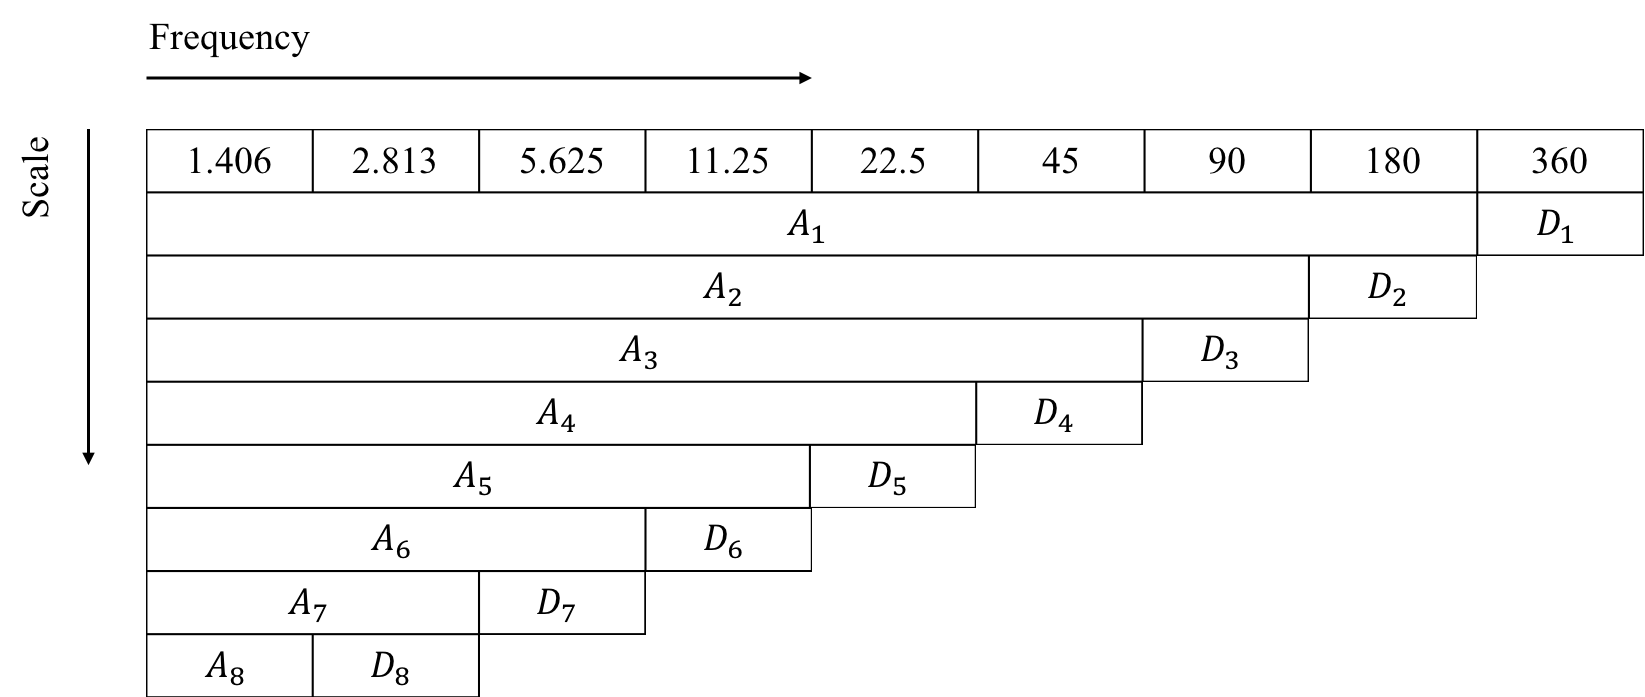
\includegraphics[scale=.5]{Fig/scale_wavelet.png}
\caption{Frequency band of wavelet decomposition coefficients for MITDB signals}
\label{fig:wavelet_decomp}
\end{figure}


The mother wavelet $db4$ is utilized at this stage due to its morphological similarity to QRS complexes. By superimposing $D_5$ and $D_6$, the QRS complex information in the ECG signal can be characterized in a one-dimensional recombined signal ($QRS\_DET = D_5+D_6$).Other Fiducial peaks (P, QRS onset, Q, S, QRS offset and T waves for each cardiac circle) are localized according to an algorithm proposed in \cite{2012qrs}. The accuracy of peak detection and its coincidence with the true signal is shown in Fig.\ref{fig:QRS_d5d6}.

\begin{figure}[t]
\centering
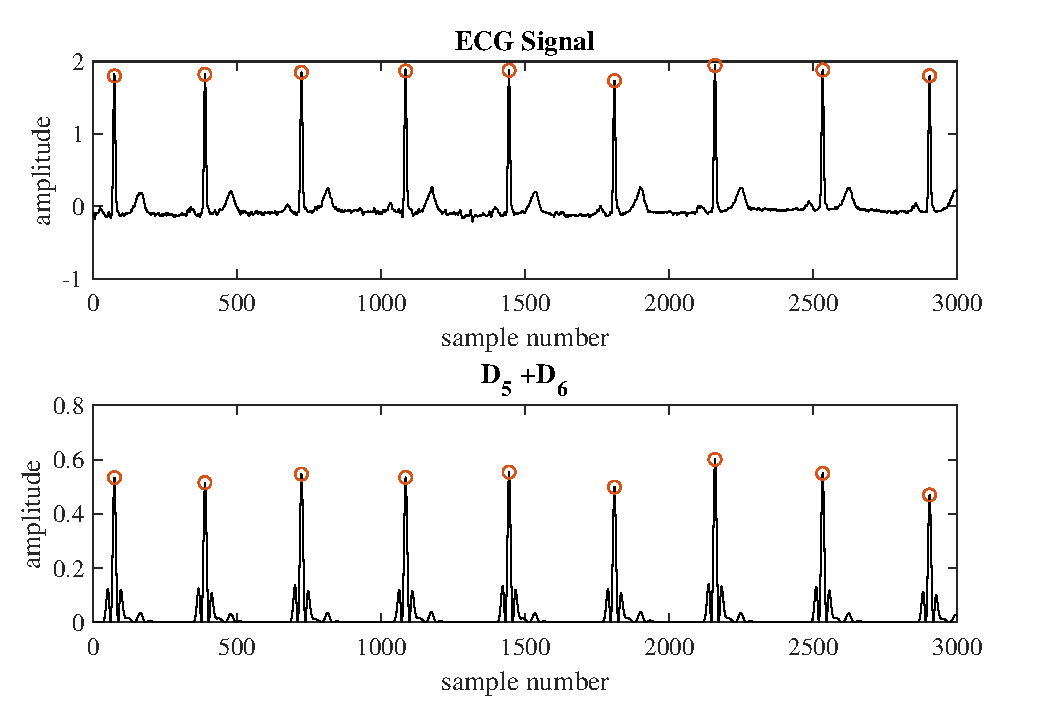
\includegraphics[scale=.7]{Fig/QRS_D5D6.pdf}
\caption{QRS detection with wavelet coefficients of level 5 and level 6. \textcolor{red}{Add dot to all captions. Also, it is good to use subfigure with captions (a) and (b) and then include the full description in the caption.}}
\label{fig:QRS_d5d6}
\end{figure}


With the empirical values described in \cite{2012qrs}, we use 15\% as the detection threshold. Since the width of most of the QRS complexes does not exceed 160ms, here we use a sliding window with a width of 160ms to detect the peaks in the $QRS\_DET$. The window step size is set to 200ms, given that the time lag between the two adjacent heartbeat cycles does not exceed 200ms.  Figure.\ref{fig:window} shows a typical $QRS\_DET$ waveform along with the corresponding window of width 160ms. The false peaks are eliminated using a 160ms time window, as seen in Figure.\ref{fig:window}.


\begin{figure}[t]
\centering
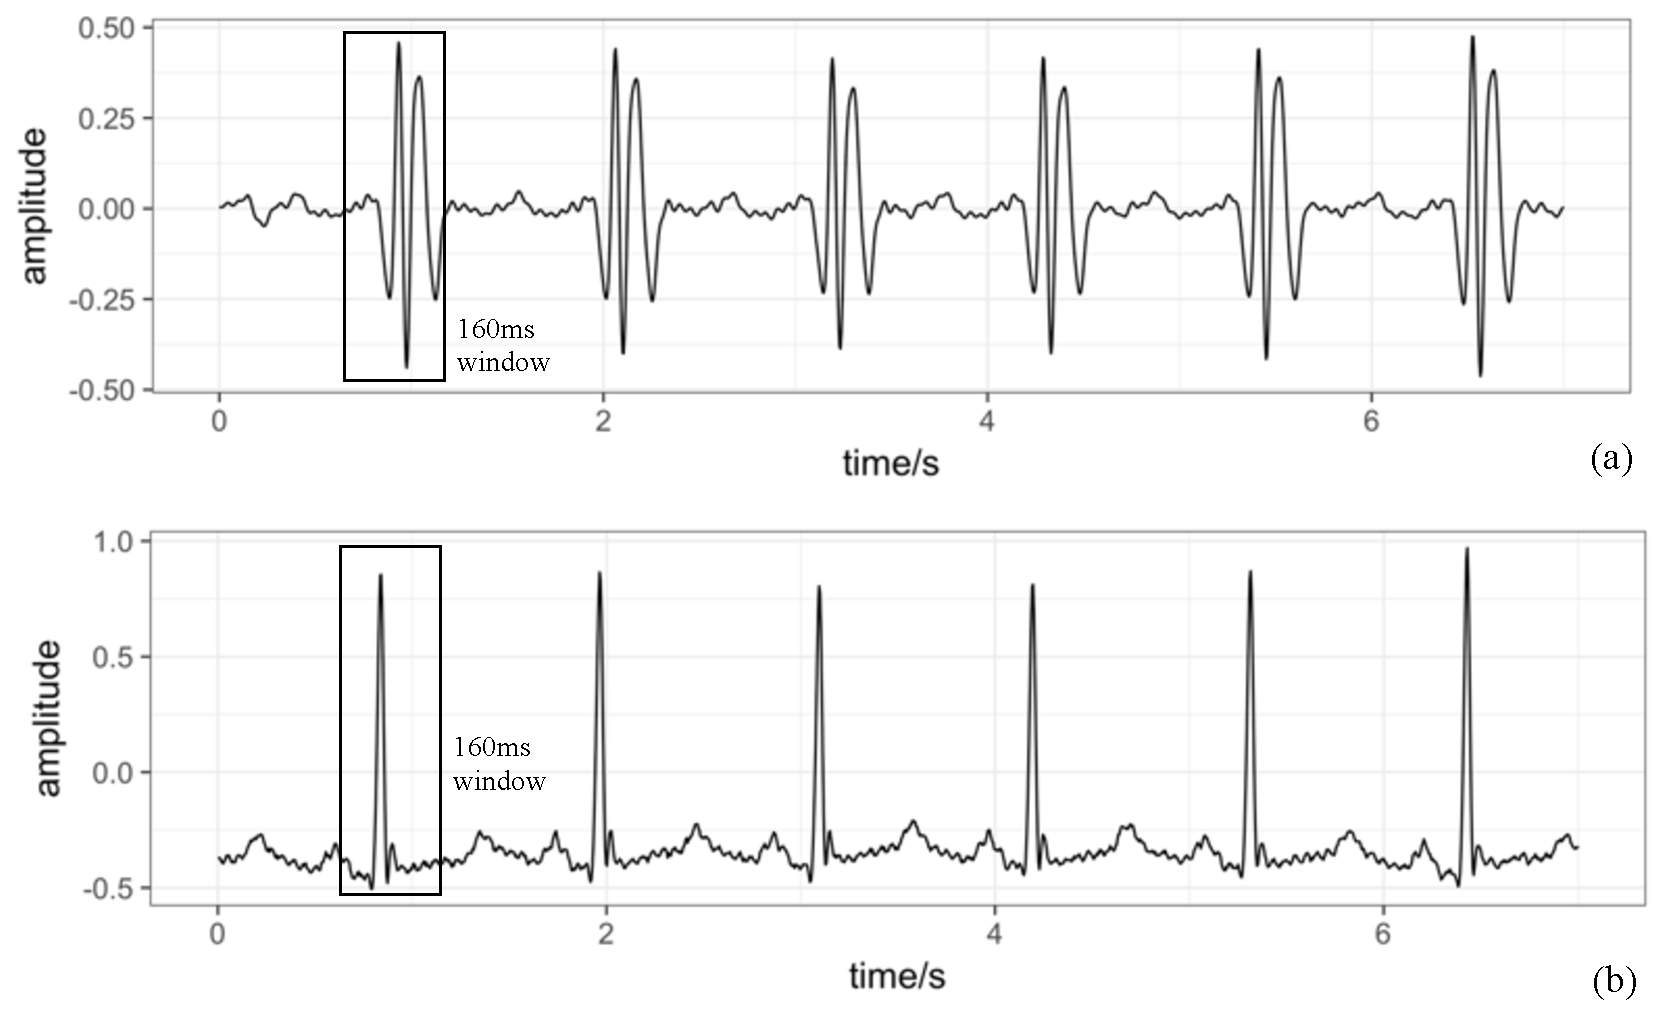
\includegraphics[scale=.5]{Fig/window.pdf}
\caption{Window for detecting R peaks within QRS complexes}
\label{fig:window}
\end{figure}


The T and P waves are outside the QRS window. Through scanning the region spanning the start of a QRS window to the end of its neighboring QRS \textcolor{red}{I think you mean: the end of a cardiac interval to the beginning of QRS window in the next interval}, the P-wave is located as the highest positive peak in this region. In a similar way, the position of the T wave is obtained by finding the maximum of the signal in the region between the from the end of the QRS in the current cardiac interval to the beginning of the next cardiac interval. \textcolor{blue}{In an alternative way, the two peaks between the two consecutive QRS windows, respectively represent the T and P waves.}
In short, an ECG signal in one heartbeat segment can be fully described by 7 feature points: P, QRS on, Q, R, S, QRS off and T. 

After localizing the feature points, we can use the location of R peaks to determine the boundaries of a cardiac cycle. %Wwave, a segment of the ECG signal was divided into cardiac cycles. 
By processing a large number of ECG signals, we realize that R peaks approximately split cardiac cycles into two pieces with $1/3$ and $2/3$ of the entire signal. \textcolor{red}{Add REF if any}. 
Based on this observation in the morphology of a typical ECG signal, we define the starting point of a cardiac cycle as the point which divides the distance between the two consecutive R waves into two sections, where the length of the first section is half the length of the second section, as depicted in Fig. {fig:interval}. In this figure, the distance (RR) between the two adjacent R waves is denoted by $h$, therefore R wave is located in distance $h/3$ with respect to the beginning of the cycle. The advantage of this method is its low computational complexity and easy generalization to different patients, noting that a slight change in cardiac boundaries do not significantly alter the properties of a cardiac cycle as long T and P waives remain in the correct interval. 

The quality of ECG signals provided by most of the portable ECG measuring instruments is very unstable and may include transient noises. Signals transmitted through wireless communication systems will exhibit even more unstable waveforms. These transient effects appear in the resulting feature vector and consequently they negatively affect the prediction accuracy of the subsequent ML method. In order to eliminate and smooth out these transient terms, we use the concept f \textit{segmentation} here, where each segment includes multiple cardiac intervals, 
%Moreover, the objective of this work is predictive modeling, thus by including statistical features capturing change between consecutive beats, the system obtains information regarding the following beats. Taking these facts into account, this work performed subsequent feature extraction and analysis combined three consecutive cardiac cycles (i.e. one representative segment). In the subsequent analysis, an segment is considered as a sample of data 
as shown in Fig.~\ref{fig:interval}. \textcolor{blue}{Note that the number of cycles in each segment is a modeling parameter shown by $XXX$. Also, we can arbitrarily slide segments equivalent to $YYY$ cycles to generate the new feature vector. The parameters $XXX$ and $YYY$ can be tuned to improve the overall performance of the method.  Based on intensive simulations, we choose $XXX=xxx$ and $YYY=yyy$, which yield the best classification accuracy. In Fig.~\ref{fig:interval}, we have $XXX=xxx$ and $YYY=yyy$.}

\begin{figure}[t]
\centering
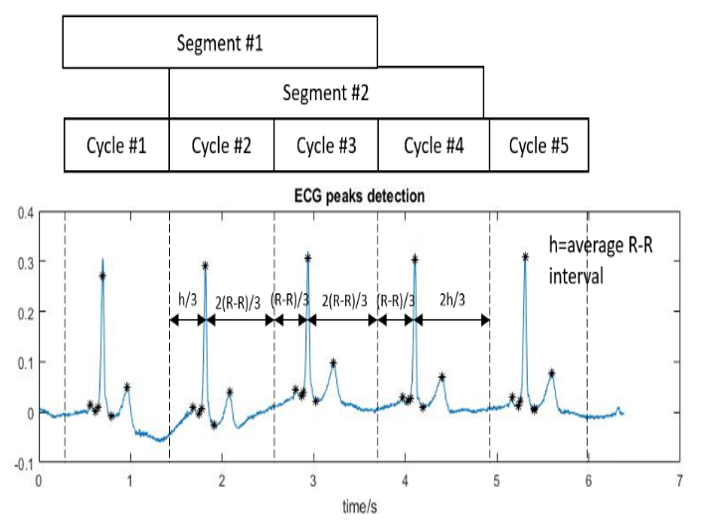
\includegraphics[scale=.8]{Fig/segment.png}
\caption{Segment samples correspond to three consecutive cardiac cycles}
\label{fig:interval}
\end{figure}


\textcolor{red}{This is not well connected to the text before and after. Make it a separate Section titled as 2.2 Utilized Dataset and move it to the beginning of this section.}
%\subsection{Dataset}
For the purpose of training and evaluating classifier, MITDB is split into test (DS2) and training (DS1) set by balancing the four classes according to \cite{autofs}. 



The ECG signals in MITDB dataset are annotated and labels are provided for each cycle. However, we define a segment, which may include more than one sample as a sample. Therefore, we need to translate per-cycle labels into per-segment samples. In this regard, a new label for each segment is generated by integrating all annotations of the beats within the segment. The segmend is labeled as \textit{normal}, if all member beats are annotated as N; otherwise, this segment will be labeled as the abnormality type of its member beats if there is only one abnormality type. If more than one abnormality types are present within the same segment, the segment is excluded. \textcolor{blue}{For instance, segments with members labels "NNN", "SSS", "NVV", "VVV" are respectively mapped to "N","S", "V", and "V", and a segment with member label "NVS" is discarded.} 
After segmentation and new annotation, the total number of samples in the training and test set are obtained as summarized in Table.\ref{table:ds}
\begin{table}[b]
	\centering
	\caption{Training and test datasets in MITDB.}
	\vspace{-0.05in}
	\begin{tabular}{|l||c|c|c|c|c|}
		\hline 
		& \multicolumn{4}{c}{Number of segments per AAMI class} &\\ 
		\hline 
		Evaluation Dataset& N & V & S & F &Total \\ 
		\hline 
		DS1:Training & 11721& 2356 & 862 & 256 & 15195\\ 
		\hline 
		DS2:Test & 12633 & 2053 & 550 & 121 & 15357 \\ 
		\hline 
		Total & 24354 & 4409 & 1412 & 377 & 30552 \\ 
		\hline 
	\end{tabular}
	\label{table:ds} 
	\vspace{-0.15in}
\end{table}

\section{Feature Extraction}

The feature extraction step plays a crucial role in the diagnosis of heart disease and has a great influence on the performance of the subsequent automated classification systems. De Chazal et al. have studied the impact of using waveform morphological features on classification results \cite{autofs}. As discussed in \cite{jambukia2015classification}, the combination of three types of characteristics (i.e. temporal, morphology, and frequency domain features) can provide a better discriminative power for the classification algorithm to distinguish between different types of arrhythmia. 

According to several studies different types of ECG signals mainly differ in the power level of the frequency band ranging from 5 Hz to 15 Hz \cite{XXX}. Likewise, some other morphological features (such as the duration between the Q wave and the T wave, P The distance to the R wave, etc.) present different levels of correlation with a specific signal classes \cite{XXX}. Therefore, we choose to use combination of temporal, morphological and spectral features as detailed in Table \ref{table:features}. Also, to account for segment-level characteristics as well as cycle-level properties, the extracted features include both periodic-based features (SET 1) and segment-based features (SET 2), where SET1 includes the average and standard deviation of the corresponding features of the three cardiac cycles within a segment, and SET2 contains the overall characteristics of the time signal within the segment, so it is calculated only once per segment. Therefore, we have a total of \textcolor{blue}{$8 \times 2 + 6 =22$} features per segment as shown in Table \ref{table:features}. Therefore, each feature vector is a $22×1$ vector with zero-mean unit-variance elements after a proper normalization. %Summarized details are described in Table.\ref{table:features}.
In Table~.\ref{table:features}, mean $(R_{i+1}-R_i)$ refers to the mean of the time lag between two adjacent R waves, while $(R_i-R_{avg})$ is the length of each cardiac cycle and the average cardiac cycle duration of the patient. 

\begin{table}[t]
	\caption{Features extracted from ECG signal\textcolor{red}{. Change column width such that each line represents one feature.}}
	\label{table:features}
	\centering
	%\begin{flushleft}
	\begin{tabular}{|m{6em} || @{}m{7.4em} ||@{} m{7.7em}|}
		\hline 
		Feature Type & SET1 & SET2 \\ 
		\hline 
		Temporal Features & QRS duration, ~~~~
		QT duration, ~~~~~~~
		PR duration & mean$(R_{i+1}-R_i)$, mean$(R_i-R_{avg})$  \\ 
		\hline 
		Morphological Features & max positive peak to second peak ratio & signal average energy, max positive peak, max
		negative
		peak, peak to
		energy ratio \\ 
		\hline 
		Frequency Domain Features & signal power level at 7.5Hz, 10Hz, 12.5Hz, 15Hz &  \\ 
		\hline 
	\end{tabular} 
	%\end{flushleft}
\end{table}

From Table.\ref{table:features}, one may notice that these 22 feature are not completely independent of each other. Also, some of the features may not be as relevant as the others. Therefore, we reduce the number of features to obtain a more robust predictive modeling \cite{Some references for feature selection}. We use Principal Component Analysis (PCA) \textcolor{red}{or principal component analysis (PCA): choose one notation} as a commonly used the common dimension reduction method instead of explicit feature selection for its improved performance in biomedical signal processing \cite{Some references for PCA as a dimension reduction method}. We keep the 8 dominant directions of the signal after PCA as the most informative 8 features.



\section{Classification Framework}

\textcolor{red}{part of the following text is related to global classifier, and part of it to deviation analysis (including personalized normal cluster, ...). Use subsections as needed to be more clear.}

In this section, we elaborate on the details of the proposed methodoology to perform the classification and prediction tasks using the pre-processed ECG data. Based on our previous study \cite{chen2018predictive} as well as similar prioir works on developing patient-specific classifiers \cite{Hu_et_al,deChazal2006,llamedo2012automatic}, we propose a two-staged structure which includes a global classifier to capture general properties of different classes followed by a personalized classifier to capture patient-specific properties~\cite{chen2018predictive,Hu_et_al,deChazal2006,llamedo2012automatic}. Moreover, the proposed algorithm incorporates a novel deviation analysis module with details presented in the following sections. 


The flowchart in Figure \ref{fig:flow} presents the overall operation of the proposed system. The \textit{global classifier} is trained using the whole training dataset as the first classification step. It facilitates the subsequent analysis in the system by identifying samples with severe morbidity. Depending on the application (properties of signals, the utilized labels, and the choice of features), different classification algorithms can be utilized \cite{REF}. Two important considerations include the classification accuracy and the computation complexity of the method \cite{REF}. Any abnormal label generated by the global classifier is considered as a \textit{red alarm} and does not require further processing. However, samples labeled as  \textit{normal} go through the subsequent personalized classification step. 

\begin{figure}[ht]
	\centering
	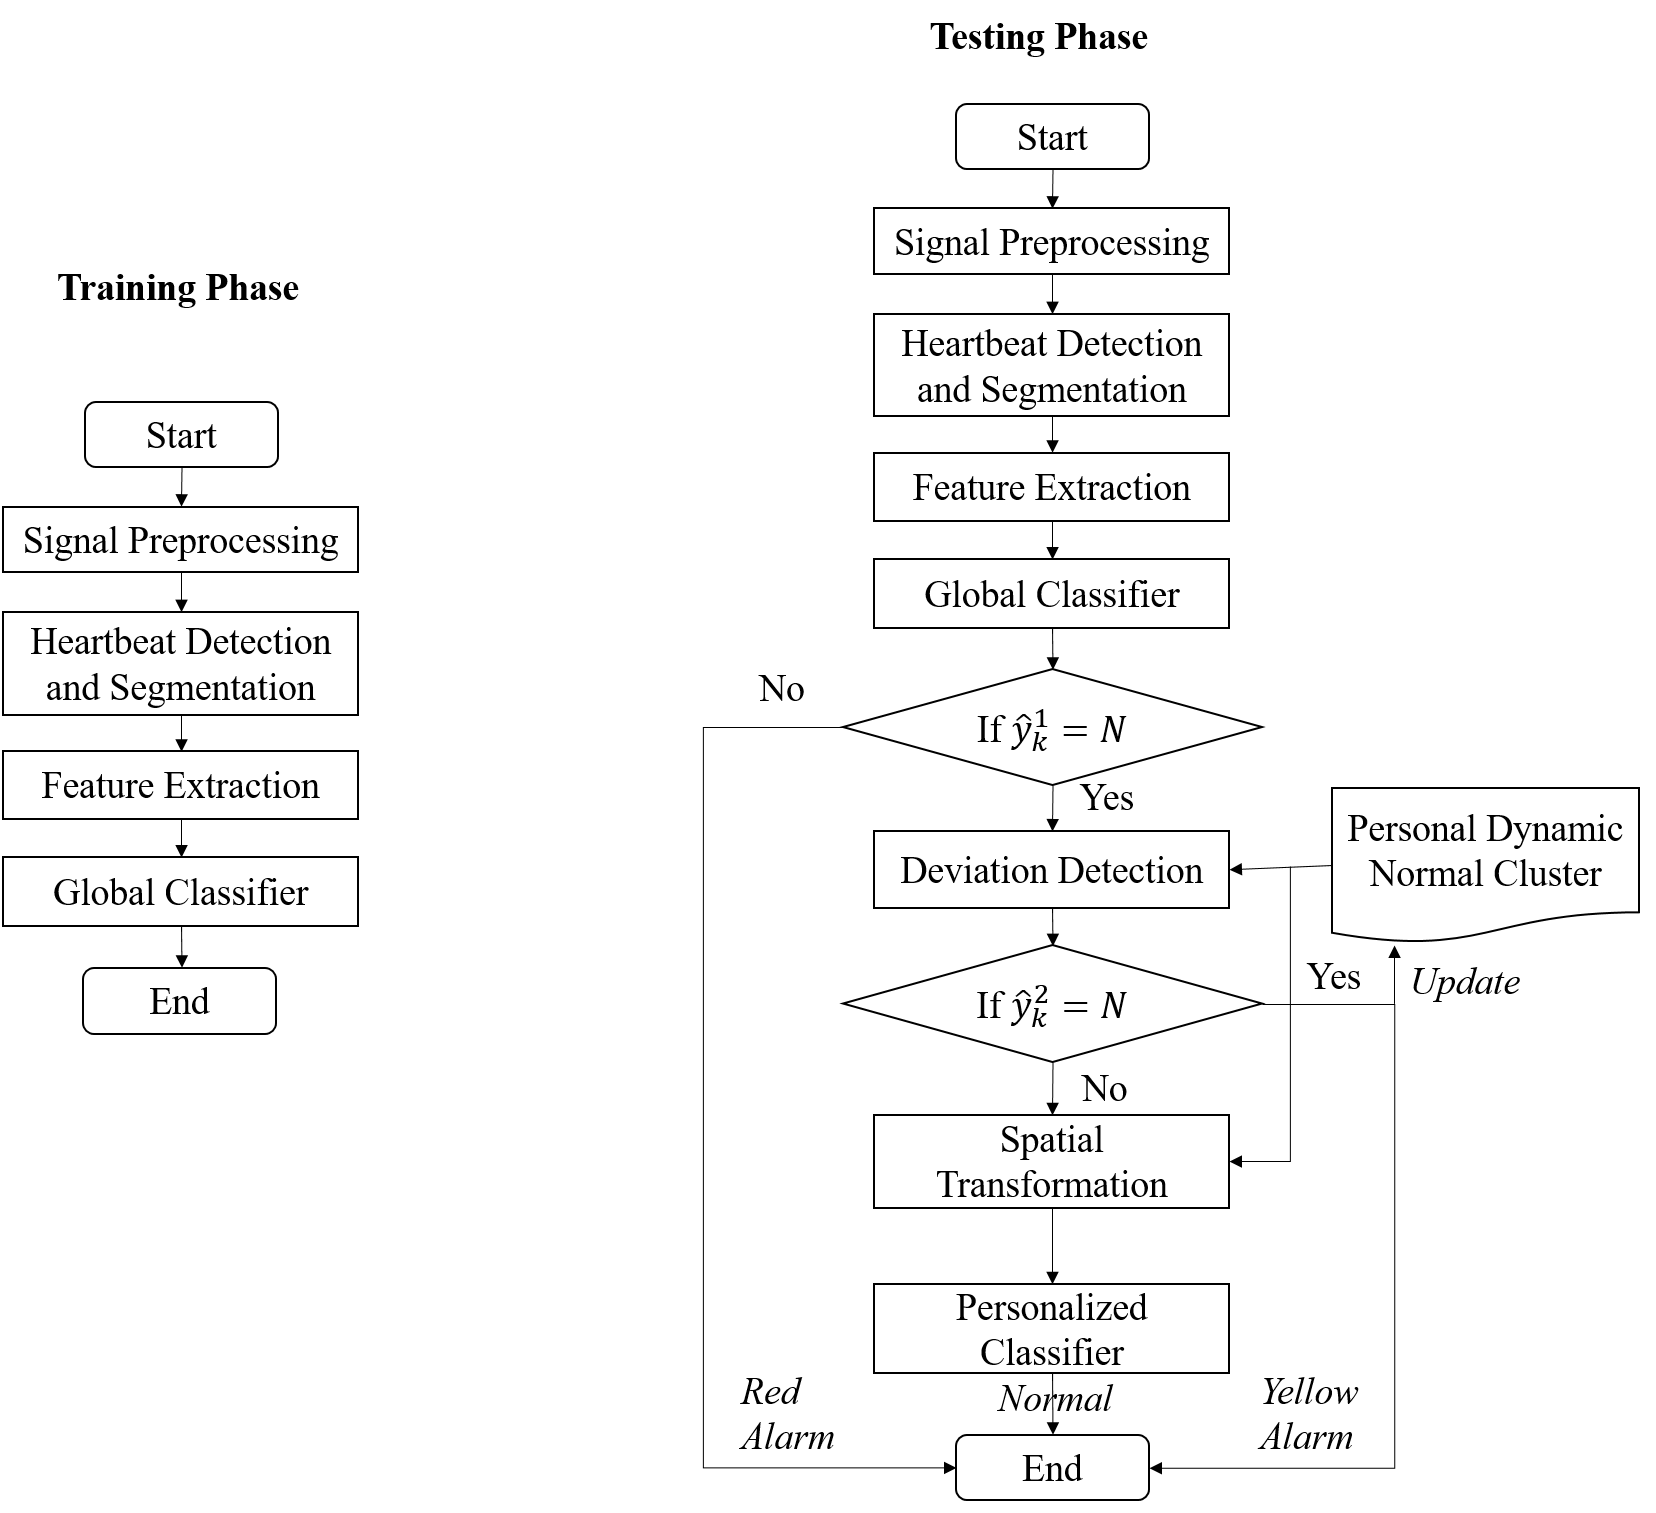
\includegraphics[scale=.5]{Fig/flow2.png}
	\caption{The general flowchart of proposed framework}
	\label{fig:flow}
\end{figure}





Since, one objective of this study is to identify the fuzzy states between normality and abnormalities, the subsequent analysis is focused on processing samples classified as \textit{normal}(N) \textcolor{red}{use a consistent notation: you can choose to use italic font for ``normal'' and ``abnormal'', ``red'', ``yellow'', etc in their first appearance or for all appearances.  Also, define labels N, S, ... on their first appearances.} to check whether or not they show considerable deviations to one of the abnormality classes. For this purpose, a one-layer classifier is not sufficient \textcolor{blue}{due to multiple reasons: i) the numbers of samples in the normal and different morbid classes are not balanced in the training set DS1 as shown in Table.\ref{table:ds}, ii) the patient-specific normal trend is not known, iii) determining yellow alarms require a new set of decision rules to determine whether or not the deviations are worthy of calling a yellow alarm.} Therefore, a deviation detection module is added after the Global Classifier to identify \textcolor{red}{latent has a special meaning in ML, which is different than what you mean., I recommend change ``latent'' to a different word} %latent status 
yellow alarms using patient-specific normal cluster. In order to develop a ground for patient-specific normal functionality and adapt the classifier accordingly, the first 20\% of total Normal samples of each patient are selected as the initialization of \textit{personalized dynamic normal cluster} $\mathcal{N}_0^k$. To do this, we use a binary classification of N versus non-N, where the second includes all abnormal classes. We firstly calculate the following distance metrics:

\begin{align}
\label{eq:matrices}
R_i^{\max}=\underset{\mathbf{x}_j\in\mathcal{N}_i^k,\mathbf{x}_k\in\mathcal{N}_i^k}{\max}\{\sqrt{(\mathbf{x}_j-\mathbf{x}_k)^2}\},
\\
D_\mathcal{X}(\mathbf{x}_k(i))=\underset{\mathbf{x} \in\mathcal{X}}{\text{median}}\{\sqrt{(\mathbf{x}_k(i)-\mathbf{x})^2}\},
\\
D_\mathcal{N}^{\max}(\mathbf{x}_k(i))=\underset{\mathbf{x} \in\mathcal{N}_i^k}{\text{max}}\{\sqrt{(\mathbf{x}_k(i)-\mathbf{x})^2}\},
%D_V(x^t)=\underset{x_V\in\Omega_V}{\text{median}}\{\sqrt{(x^t-x_V)^2}\}\\
%D_S(x^t)=\underset{x_S\in\Omega_S}{\text{median}}\{\sqrt{(x^t-x_S)^2}\}\\
%D_F(x^t)=\underset{x_N\in\Omega_F}{\text{median}}\{\sqrt{(x^t-x_F)^2}\}\\
%D_{max}(x^t)=\underset{x_N\in\Omega_N^t}{\max}\{\sqrt{(x^t-x_N)^2}\}
\end{align}

The following conditions are then examined to verify if the deviation of a sample is within the range defined by $\alpha$. Since some rare abnormalities are unlikely to be observed within the limited initialization period, therefore abnormal clusters: ${\mathcal{S},\mathcal{V},\mathcal{F}}$, which include abnormal beats for all patients in DS1, are deployed as the training dataset when developing the  \textit{personalized dynamic normal cluster} $\mathcal{N}_i^k$ as follows. \textcolor{red}{I think here in $\mathcal{N}_i^k$, you mean that $i=0$ represents the normal cluster and $i=1,2,...$ represent different abnormality clusters. This is not obvious and you need define it before its first appearance.}

\begin{align}\label{eq:condition1}
\begin{cases}
D_\mathcal{N}^{\max}(\mathbf{x}_k(i))  \leq\alpha R_i^{\max},\\
D_\mathcal{N}(\mathbf{x}_k(i)) < D_\mathcal{X}(\mathbf{x}_k(i)) &\text{for~} \mathcal{X}\in\{\mathcal{S},\mathcal{V},\mathcal{F}\}   %(D_N(x^t),D_V(x^t),D_S(x^t),D_F(x^t))=D_N(x^t)
\end{cases}
\end{align}

If a sample already called normal by the global classifier, is again confirmed as N in this module, it will be used to update the $\mathcal{N}_i^k$. Otherwise, the system assumes that the sample has a considerable deviation towards one of the abnormal clusters and hence will pass it to the subsequent \textcolor{blue}{\textit{personalized classifier}}. The \textit{personalized classifier} uses controlled transformation with optimized parameters to discern the deviation to different morbid types regardless of the cluster topology within the original feature space \textcolor{blue}{, as detailed in Section XXX}. 

After performing both global and personalized classification steps, a given sample $x_k$ at time $k$ is mapped to label $\hat{y}_k \in \{N,Y_V,Y_S,Y_F,R_V,R_S,R_F\}$, where $N$ stands for normal status, $Y_X$ stands for a ventricular yellow alarm of type ``X'', and $R_X$ stands for a ventricular red alarm of type ``X''.

\begin{figure}[t]
\centering
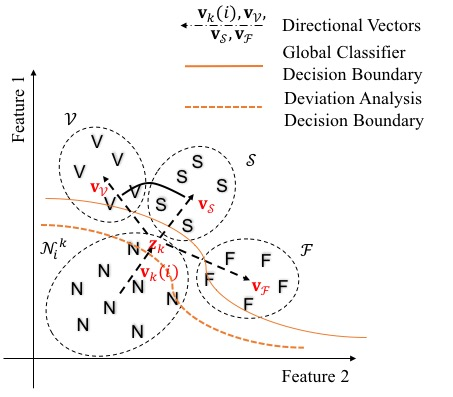
\includegraphics[scale=.7]{Fig/topology.jpg}
\caption{The deviation analysis boundary restrict on latent status between normal and abnormal samples compared with the Global Classifier boundary}
\label{fig:topo_deviation}
\end{figure}


\section{Personal Classifier} \textcolor{red}{I suggest you use the term personalized classifier, although personal classifier is correct too.}

Here, we provide the core idea behind the design of the personalized classifier, and the details of implementation will be discussed in \textcolor{blue}{Chapters 3 and 4.} 
Since the proposed system aims at predicting subsequent abnormalities by analyzing a signal's deviation from the patient's normal functionality of the sample signal, it is vital to quantify the deviations using topological characteristics of the training dataset. For most of the ECG applications, ECG signal is analyzed by its representative feature vectors. A natural choice for deviation analysis in the high-dimensional feature space, is Cosine Distance \textcolor{blue}{\textit{cosine distance}} as defined in Eq.\ref{eq:cosine}) to quantify the distance between two vectors $\textbf{v}$ and $\textbf{w}$.

\begin{align}
\label{eq:cosine}
d(\mathbf{v},\mathbf{w})= 1 - \frac{\mathbf{v}^T\mathbf{w}}{|\mathbf{v}||\mathbf{w}|}=1 - \frac{\mathbf{v}^T\mathbf{w}}{\sqrt{(\mathbf{v}^T\mathbf{v})(\mathbf{w}^T\mathbf{w})}}
\end{align}

Consequently, relative deviations of a sample from normal cluster(N) to other abnormal clusters (V, S, F) are defined by the cosine distance between the vector $\mathbf{v}_k(i)$ (defined in Eq.\ref{eq:v_k}) and the three vectors $\mathbf{v}_{\mathcal{X}}(i)=\mathbf{c}_{\mathcal{X}}-\mathbf{x}_k(i)$ where $\mathcal{X} \in \{ \mathcal{S}, \mathcal{V}, \mathcal{F}\}$. \textcolor{blue}{In this case, a smaller cosine distance represents a higher alignment between the vector from the normal cluster centroid $\mathbf{v}_k(i)$ to the current sample $\mathbf{x}_k(i)$ and the reference vector from the normal cluster centroid to abnormal centroids $\mathbf{c}_{\mathcal{X}}$.}


\begin{align}
\label{eq:v_k}
%\mathbf{v}_k=\mathbf{x}_k-\mathbf{c}_N^k = \mathbf{x}_k- \frac{\sum_{j=1}^{k-1} \mathbf{x}_j I(\hat{y}_j=N)}{\sum_{j=1}^{k-1}  I(\hat{y}_j=N)}, 
\mathbf{v}_k(i)=\mathbf{x}_k(i)-\mathbf{c}_N^k(i) = \mathbf{x}_k(i)- {\sum_{\mathbf{x} \in \mathcal{N}_i^k} \mathbf{x}}/{|\mathcal{N}_i^k|}, 
\end{align}

Therefore, the classification result of the Personal Classifier $\hat{y}^2_k(i)$ is determined as follows:

\begin{align}
\label{eq:personal_discrim}
\hat{y}^2_k(i) = \underset{\mathcal{X} \in \{ \mathcal{S}, \mathcal{V}, \mathcal{F} \}}{\text{argmin}}\{ d(\mathbf{v}_k(i),\mathbf{v}_{\mathcal{X}}(i)) \} 
\end{align}

The relevance of cosine distance depend on the topology of clusters in the feature space. The topology in feature space, itself is inherited from the feature extraction and feature selection methods. For example, as shown in Fig.\ref{fig:topo1}, in the original feature space overlaps and alignment of abnormal clusters may lead to inaccurate results of deviation quantification. \textcolor{blue}{In order to eliminate the deviation analysis errors that arise from the asymmetry in the clustering topology, it is desired to transform the original topology into a more symmetric topology, where cosine distances directly reflect the amount of deviations.}

\begin{figure}[thpb]
\centering
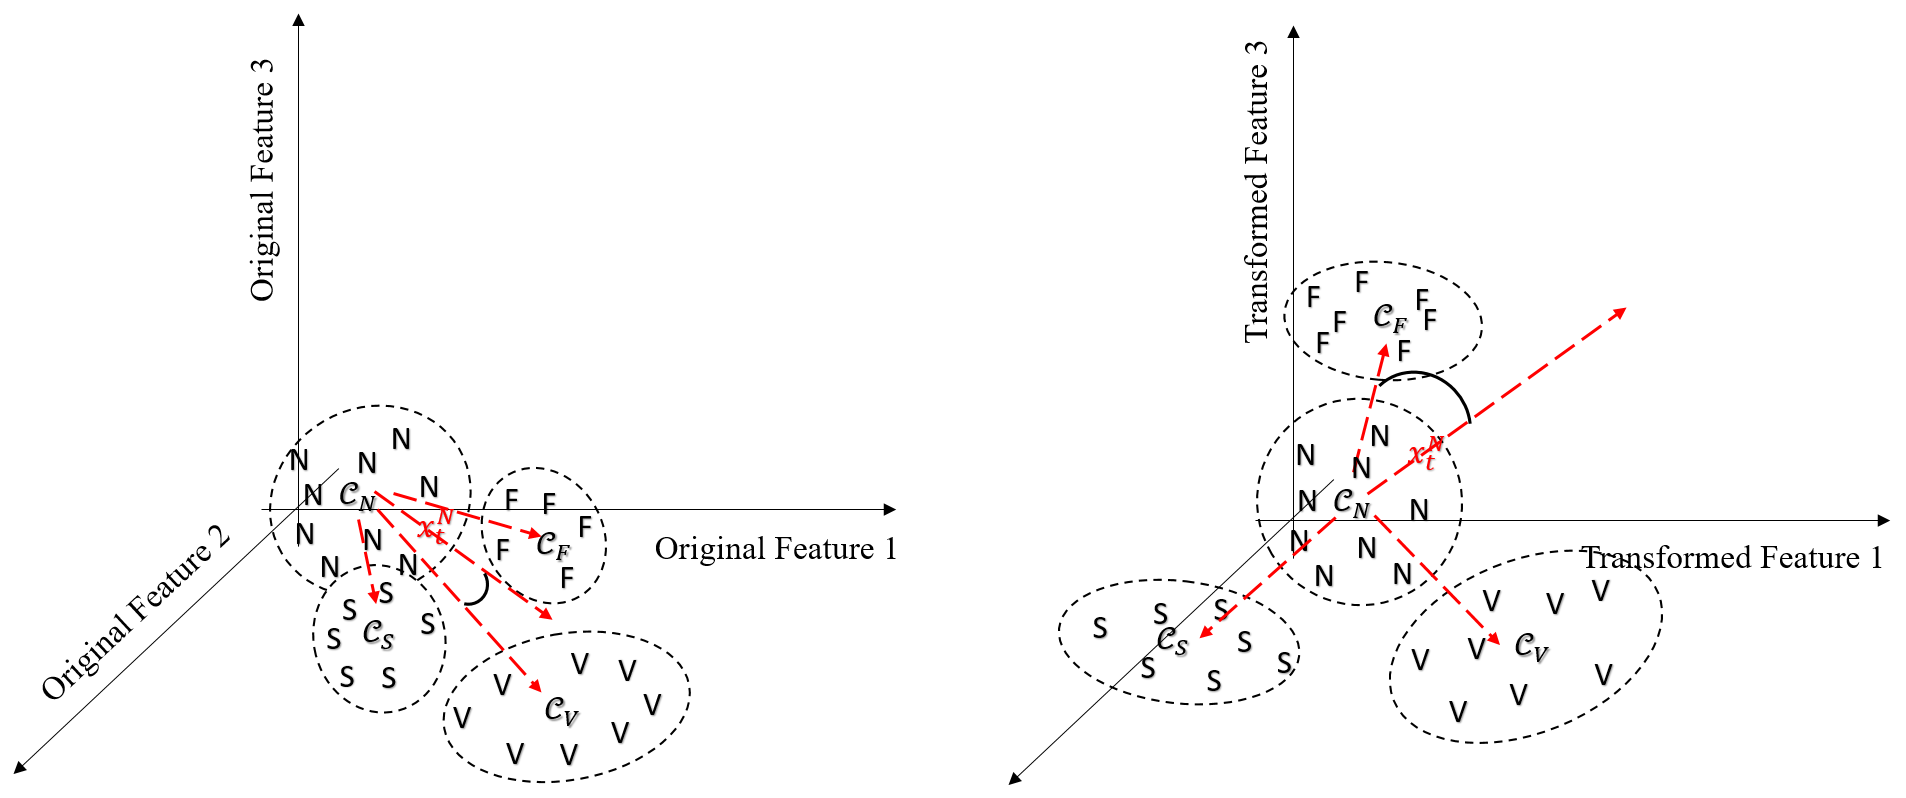
\includegraphics[scale=.5]{Fig/topo1.png}
\caption{Left: illustration of the cluster topology in the original feature space; Right: illustration of the cluster topology in the transformed feature space using a nonlinear mapping function.}
\label{fig:topo1}
\end{figure}

For this purpose, two different spatial transformation methods are proposed in the next two chapters.


%\chapter{\textit{Kernels}-Based Nonlinear Spatial Transformation}\label{ch:spheremapping}
\section{Introduction}

As discussed in Chapter 2, the main objective of the personalized classifier is to reassess the normal samples to identify deviation of seemingly normal samples into any of abnormality types. \textcolor{blue}{The original geometry of clusters in the feature space $\Omega^d$ depends on the choice of features implied by the feature extraction and feature selection stages $g()$}. We noticed that with the resulting features (in this work), the clustering geometry does no exhibit the necessary symmetric property and thus leads to a poor performance and even failure in predicting subsequent abnormalities. 
Therefore, an optimization method based on spatial transformation is proposed to solve this issue. More specifically, we propose a method to reshape the clusters such that 
 \begin{itemize}
\item The abnormal classes surround the normal class; 
\item A maximal separation among the abnormal classes are achieved; 
\item The angles between the vectors connecting the centroid of normal cluster to different abnormal clusters are equalized. 
\end{itemize}

These properties can be achieved through imposing the following conditions:  
 \begin{itemize}
     %\item Vectors pointing from normal centroid to different abnormal clusters centroids has no overlapping or cross with each other.
     \item Vectors pointing from the normal centroid to different abnormal clusters centroids present maximum mutual cosine distances.
     \item The overlapping parts among all clusters are minimized.
 \end{itemize}

% maximizing the minimum of the angles between the aforementioned vectors from the normal cluster centroid to abnormal cluster centroids. 


Given that the clusters in original feature space do not meet these symmetric properties, developing a spatial transformation is unavoidable. In this chapter, a \textit{kernel}-based nonlinear spatial transformation is proposed to reshape the feature space to reach the above-mentioned required symmetric properties. 
%Here, we assume in this chapter that new feature space obtained by non-linear reshaping is noted as $\Phi^{d'}$. 
\textcolor{blue}{This reshaping process is part of the \textcolor{blue}{\textit{personalized classification}} stage (as shown in Fig.\ref{fig:flow}) of the ECG classification system as described in chapter 2. The nonlinear mapping projects the corresponding feature vector of each sample $\mathbf{x}_k$  in the original space $\Omega^d$ onto a new vector $\mathbf{z}_k$ in a higher dimensional space denoted by $\Omega^{d^\prime}$.  This is achieved using a nonlinear mapping function $\Phi^{d'}:\Omega^{d} \rightarrow \Omega^{d^\prime}$. The resulting vectors are used by the personalized classifier to identify the minor yellow alarm type out of $\{\mathcal{N},\mathcal{S},\mathcal{V},\mathcal{F}\}$.}
\textcolor{red}{
The original text was ambiguous. Firstly, set and cluster shapes can be viewed differently, sets are not changes under the transformation although cluster geometry changes. Therefore, since we already used $\mathcal{N},...$ to represent clusters in the original space, you can use $\mathcal{N'},....$ for the transformed clusters, unless you mean a set (not a cluster). In this case, sets do not changes under the transformation, and you can omit the definition $\Phi^{d'}=\{\mathcal{N},\mathcal{S},\mathcal{V},\mathcal{F}\}$ to avoid ambiguity.
Secondly, you need to distinguish between two functions, one simply maps the vector in original space into a new space, and the second one processes the transformed vector and maps it to a yellow alarm. It is not clear in the text.}

%  which can be considered as the union of subspaces for transferred types: %$\Phi^{d'}=\{\mathcal{N},\mathcal{S},\mathcal{V},\mathcal{F}\}$, where $d'>d$. 
  

\section{\textit{Kernel} Method}

Kernel method has been widely used in machine learning algorithms. For instance, it is the integral part of nonlinear Support Vector Machine (SVM), which has been utilized in numerous applications recently\cite{shawe2004kernel}. Nonlinear kernel methods can efficiently improve the classification performance when there exists a nonlinear relationship between the input and output variables. Because of the complexity and diversity of feature vectors used in ECG analysis, the assumption of nonlinear relationship is considered valid in this work. Therefore, incorporating nonlinear kernel methods in the ECG analysis system, can be beneficial.

In kernel SVM, the nonlinearities are introduced to the model through a kernel function, which implicitly maps data points $\mathbf{x_i} \in \mathcal{X}$ in the input space $\Omega$ into a Hilbert space $\Phi$ via a nonlinear function $\Psi()$\cite{aronszajn1950theory}. Then, the algorithm minimizes the expected error $E[L(y,f(x)]$ between the true labels $y$ and the predicted values $f(x)$ for samples in a training dataset, by finding an optimal classification function $f$, which also depend on the choice of $\Psi()$. Here, $L()$ is an arbitrary loss function, and a popular choice is the least squared errors $\sum\limits_{x_i \in \mathcal{X}} (y_i-f(x_i))^2$ \cite{scholkopf1999advances}. \textcolor{red}{Other choices for loss function include Hindge loss, absolute loss, hit and miss loss, etc [REF]}.

If there are $m$ observations in the input space, we use notation $\mathbb{N}$ for index set ${1:m}$. Based on the input space $\mathbf{x_i}\in \Omega (i\in \mathbb{N})$ and classification mapping function $f$, the optimization problem can be written as:
\textcolor{red}{better to use $n$ instead of $m$ if it does not conflict with other definitions.}
\begin{align}
    \text{minimize}~\frac{1}{m}\sum_{i\in \mathbb{N}}L(y_i,f(\mathbf{x_i})) + \gamma||f||^2,
    \label{eq:kernel}
\end{align}

where $||f||^2$ is the squared norm of $f$ \textcolor{red}{here f is a function and norm is defined for vectors. So add one or two sentences how to calculate it. I think for instance you mean the norm of coefficients of a polynomial function here.}% on Hilbert space $H_K$. 
and the positive constant $\gamma$, also known as the regularization parameter, controls the balance between training error and the model complexity (smoothness).



%For example, if $H_K$ is the Hilbert space of linear functions, the $f$ can be written as $f=w' x,~w\in\mathbb{R}^d$. Therefore, the loss function can be written as:

%\begin{align}
%    \frac{1}{m}\sum_{i\in \mathbb{N}}L(y_i,w'\mathbf{x_i}) + \gamma w'w
%    \label{eq:kernel}
%\end{align}

%Positive constant $\gamma$, also known as the regularization parameter, controls the balance between training error and the model complexity (smoothness). 
When optimizing the above objective function, SVM only requires the inner products of the transformed features $\Psi(\mathbf{x})$ in the Hilbert Space $\Phi$. Therefore, a kernel defined as $k(\mathbf{x_i},\mathbf{x_j}) = \Psi(\mathbf{x_i})^T\Psi(\mathbf{x_j})$ can efficiently substitute the inner product calculation and induces the necessary nonlinearities into the model\cite{evgeniou2000regularization}.

%In SVM and other machine learning models, nonlinear kernel methods are implemented with different loss functions \cite{evgeniou2000regularization}. But in more general conditions, the solution to Eq.\ref{eq:kernel} can be written as follows: 

%\begin{align}
%    f(x)=\sum_{i\in \mathbb{N}}c_i K(\mathbf{x_i},\mathbf{x} )
%    \label{eq:kernel2}
%\end{align}

%where ${c_i: i \in \mathbb{N}}$ is a set of real number, $K$ is a kernel such as a polynomial kernel of order $r$: $K(x,t)=(x't)^r,~x,t\in \mathbb{R}^d$.

%For any kernel $K$, it has the following properties: i) for $\mathbf{x} \in \Omega$, $K(\mathbf{x},\cdot)\in H_K$; ii) for $f\in H_K$, $<f,K(\mathbf{x},\cdot)>_K = f(\mathbf{x})$, where $<\cdot,\cdot>_K$ represents the inner product of $H_K$\cite{aronszajn1950theory}.

%A kernel is usually defined base on feature mapping concept, in this work we define this mapping function as $\Psi:\Omega^d\to \Phi^{d'}$ %where $\Psi^{d'}$ is Hilbert space and $<,>_{\Phi}$  represents inner product. 
%Therefore, Eq.\ref{eq:kernel2} can be also written as:

%\begin{align}
%    f(x) = \sum_{i\in \mathbb{N}}c_i \Psi(x_i,x)
%\end{align}



Different \textit{kernels} represent different nonlinear mapping functions. For machine learning models, the selection of kernel plays a crucial role. Therefore is no straightforward method to choose the best kernel and it is typically chosen by try and error and other heuristic model selection methods. An effective kernel function generally needs to satisfy Mercer conditions, so that the inner products can be replaced by kernel functions, as used in SVM \cite{cristianini2000introduction}. 
%This means the matrix defined by function $\Psi(x_j,x)$ is symmetric positive semi-definite. In general, the selection of kernel function depends on all observations in input space. 
An exhaustive search for all possible kernels is a computationally expensive and unrealistic task\cite{chapelle1999support}. A more efficient way to resolve this issue would be to search for an optimally weighted combination of a set of base kernels, such as polynomial kernel function and Gaussian kernel function\cite{lanckriet2002robust}. This method has been proven to be robust and efficient since the base kernels satisfy Mercer’s condition individually and it can be consistent with different datasets\cite{jebara2004multi}.
%However, in effect, kernel functions with simple expression, such as polynomial kernel function, Gaussian kernel function and exponential kernel function are usually preferred than complicated kernel function for its simplicity and consistency. 


Polynomial kernel is usually applied on normalized data for its explicit expression and steady performance. However, the degree of freedom in defining a polynomial kernel is relatively high, which requires tuning a large number of parameters. \textcolor{red}{In fact this statement is not so relevant here. Note that a polynomial kernel of order $p$ can be defined as $(1+v^Tw)^p=(1+v_1w_1+v_2w_2+...)^p$, which has only one free parameter $p$ and all coefficients are automatically determined. However, we are going to use a polynomial function of order $p$, (i.e. $f(v)=1+\alpha_1 v_1+\alpha_2 v_2+...+ \alpha_i v_1^2 + \alpha_j v_1v_2+... \alpha_k v_N^p$) which obviously required tuning too many free coefficients $\alpha_i$.}

Gaussian kernel function \textcolor{red}{denoted by XXX for vectors v and w} is a very classic robust radial function, which has shown a string robustness in the case of noisy datasets [REF XXX]. However, it is equivalent to the inner product of samples after projecting into an infinite dimensional space; therefore it is difficult to visualize the projected observations $\Psi(\mathbf{x})$ and interpret the results. %Moreover its performance is greatly affected by parameter selection.

Considering the above-mentioned facts, in this work, the polynomial kernel is selected for the purpose of validating the proposed method and interpreting the effect of an optimized nonlinear kernel method on feature space reshaping. However, the proposed methodology is general and applicable to other nonlinear kernels.

The mapping function, which is a weighted combination of polynomial kernels can be explicitly written in the following format:

\begin{align}
\mathbf{z}_k
=\mathbf{\Psi_{w}} (\mathbf{x}_k) = 
\begin{bmatrix}
w_{1}  \\
w_{2}   \\
\vdots \\
w_{d^\prime} 
\end{bmatrix}
\circ
\begin{bmatrix}
\psi_1(\mathbf{x}_k)\\
\psi_2(\mathbf{x}_k)\\
\vdots\\
\psi_{d^\prime}(\mathbf{x}_k)
\end{bmatrix} \color{red}{,}
\label{eq:z}
\end{align}
where $\mathbf{w}$ is the vector of \textcolor{blue}{normalized} coefficients \textcolor{red}{do we have $||w||=1$}. Instead of selecting kernel, %The example above shows that regardless the selection of kernel function, parameter optimization will play a critical role. For instance, in this work, 
the process of spatial geometry optimization is accomplished by adjusting the coefficients of fixed polynomial basis functions $\psi()$. Since the number of free parameters increases exponentially with the order of polynomial function, an exhaustive search is not practical for parameter optimization. Therefore, it is necessary to implement a heuristic optimization algorithm, in which parameters are obtained by maximizing or minimizing an objective function. More specifically, the nonlinear reshaping module in this chapter aims to adjust mapping coefficients  $\mathbf{w} = [w_1,w_2,\dots w_d]^T$ to achieve the ideal symmetric geometry in the reshaped feature space while maintaining the maximal separation between clusters.


\section{Multiobjective Optimization}

\subsection{Objective Functions}

To elucidate the details of the optimization problem, here we consider an illustrative example, where the original feature space is a 2-dimensional space $\Omega^2$. \textcolor{red}{This is not necessarily true, since you can choose any order of power even for a 2-D input vector. Therefore, the mapping base kernel may adopt a second-order polynomial function as follows:}
We also assume for simplicity that the order of the polynomial function is 2. Therefore, we have:

\begin{align}
\nonumber
&\mathbf{x}=[x_1~ x_2]^T,~~ \mathbf{w}=[w_1~ w_2~ \dots~ w_5]^T,~~d=2, ~~d^\prime=5,\\
&\psi_1(\mathbf{x})=x_1, \psi_2(\mathbf{x})=x_2, \psi_3(\mathbf{x})=x_1^2, \psi_4(\mathbf{x})=x_2^2, \psi_5(\mathbf{x})=x_1x_2.
\label{eq5}
\end{align}
\textcolor{red}{when you start the sentence with ``where'', it means that the equation is connected to the following sentence, so it is better to add a comma to the end of equation. Otherwise, add dot ``.''. I fixed some, but make sure that you do it consistently.}


Inspired by the way loss functions are used in the SVM methods with a non-linear kernel, we use the following objective functions in order to impose the symmetry and separation of different abnormality classes in the proposed optimization problem: \textcolor{red}{I think, you mean LDA classification, Fisher discriminant function here where SW/SB is used. I don't see any relation to SVM. Modify this part to be clear and accurate.}

\begin{align}
\label{eq:obj}
&o_1(\mathbf{w}) = \frac{1}{\underset{c,d=2,\dots,p \text{ and } c\neq d }{\min}\{d(\mathbf{v}_{\mathcal{X}_c},\mathbf{v}_{\mathcal{X}_d})\}} \\ %|a,b=1,2\dots k;a\neq b)
\nonumber 
&o_2(\mathbf{w}) = \frac{SW}{SB}=\frac{\sum_{c=1}^{C}  \sum_{\mathbf{z} \in \mathcal{X}_c}   (\mathbf{z}-\mathbf{c}_{\mathcal{X}_c})^T(\mathbf{z}-\mathbf{c}_{\mathcal{X}_c})}{\sum_{c=1}^{C}\sum_{d=1, d\neq c}^{C}  (\mathbf{c}_{\mathcal{X}_c}-\mathbf{c}_{\mathcal{X}_d})^T(\mathbf{c}_{\mathcal{X}_c}-\mathbf{c}_{\mathcal{X}_d}) }
\end{align}

The maximization of pairwise cosine distance between the vectors $\mathbf{v}_{\mathcal{X}_{c,d}}$ connecting the centroid of the normal cluster to the centroids of abnormal clusters $\mathcal{X}_c$ is achieved by minimizing $o_1(\mathbf{w})$. In fact, this objective functions is deduced from discrimination function of personal classifier in Eq.\ref{eq:personal_discrim}. Cosine distance is defined by Eq.\ref{eq:cosine} and the calculation of $\mathbf{v}_{\mathcal{X}_{c,d}}$ can be written as follows: %In the formula, vectors used to measure symmetry is defined by abnormal sample sets in training set DS1 and the personal normal cluster as follows:

\begin{align}
\mathbf{v}_{\mathcal{X}_i} = \mathbf{c}^k_N -  \mathbf{c}_{\mathcal{X}_i}
\end{align}

Since for some patients, the total number of a certain type of abnormal samples are very limited, the abnormal samples in training set DS1 are utilized in calculating the two objective functions. In Eq.\ref{eq:obj}, the abnormal cluster centroids are calculated using the abnormal samples in training dataset DS1, while the centroid of the normal cluster is defined by the \textcolor{blue}{preceding normal samples for the same person}. %personal normal cluster. 

On the other hand, $o_2(\mathbf{w})$ represents the ratio of the within-cluster variance to the between-cluster variance and consequently controls the separation between the clusters. By minimizing $o_1(\mathbf{w})$ and $o_2(\mathbf{w})$ jointly, the algorithm eliminates the ambiguity of classification while %using Eq.\ref{eq:personal_discrim} to discriminate latent abnormal state and improves the predictive capability.
improving the predictive power of the personalized classifier due to the symmetric geometry of clusters. 

\subsection{Multi-objective Particle Swarm Optimization}

We notice that $o_1(\mathbf{w}) $ and $o_2(\mathbf{w})$ are not necessarily independent of each other. Thus, the optimization problem defined above is equivalent to joint minimization of $o_1(\mathbf{w}) $ and $o_2(\mathbf{w})$ subject to a constraint condition: $|w|_2=1$. This constraint is necessary since the first objective function $o_1(\mathbf{w})$ is inversely proposal to $|w|_2$, whereas the second objective function $o_2(\mathbf{w})$ is scale-invariant. 

This problem is a non-convex multi-objective optimization problem. Therefore, neither closed form solutions nor the optimization methods proposed for convex problems are applicable to this case. In this work, we utilize \textit{multi-objective particle swarm optimization} (MOPSO) algorithm to solve this optimization problem and obtain the optimal coefficients \cite{Mo-PSO}.

\textit{Particle swarm optimization} (PSO) is based on heuristic search and has the advantage of fast convergence, and easy implementation\cite{coello2002mopso, alvarez2005mopso}. PSO is defined to solve problems with a single objective function, where closed form solutions are not tractable.  Several research works are devoted in the past decade to extend this method to multi-objective optimization problems \cite{XXX: Add REFs here if there are other implementations of MO-PSO}. In the MOPSO framework, the goal is to solve the typical \textit{Pareto optimization problem} based on the evolutionary algorithm used in PSO. In other words, it aims at solving an optimization problem with two or more conflicting objective functions by approximating the \textit{Pareto front}. 

%\subsubsection{Pareto Front} 

In order to compare different set of coefficient in this opmization problem, the concept of Pareto front is briefly introduced in this section. For a multiobjective optimization problem with two objective function, if a solution $\mathbf{w}^1$ is said to \textit{dominate} another $\mathbf{w}^2$ when the following two conditions are satisfied:
\begin{enumerate}
    \item $o_1(\mathbf{w}^1) \leq  o_1(\mathbf{w}^2)$ and $o_2(\mathbf{w}^1) \leq  o_2(\mathbf{w}^2)$ 
    \item $o_1(\mathbf{w}^1) <  o_1(\mathbf{w}^2)$ or $o_2(\mathbf{w}^1) < o_2(\mathbf{w}^2)$ 
\end{enumerate}

If a solution is not dominated by any other solutions in the searching space, then this solution is an \textit{optimal} solution for this problem. A Pareto front is defined by the set of Pareto optimal solutions. However, in non-convex optimization, the Pareto front can not be represented explicitly by a deterministic function. Therefore, the majority of algorithms use heuristic searching algorithms to approximate the Pareto front\cite{coello2002mopso}.

\subsubsection{MOPSO} \textcolor{red}{change subsection title here since it is exactly equal to the section title. You may use: implementation details of MOPSO, ....}

Among different implementations of MOPSO, the algorithm proposed by Coello Coello and Lechug presents a better performance and lower computational complexity in most applications\cite{coello2002mopso}. Therefore, this algorithm is implemented and utilized in this work to solve the multi-objective optimization problem. One special property of this algorithm is the use of external repository, in which all Pareto optimal particles for every swarm is recorded for each iteration. The solution represented by repository members are stored and used as an optimal approximation of the Pareto front because they converge to the actual Pareto front as proved in \cite{coello2002mopso}. \textcolor{red}{You may add a few more sentences here regarding the operation of MOPSO such that it is easily understandable for a general reader.}



Fig.\ref{fig:repo_members} presents the results of joint minimization of objective functions $o_1(\mathbf{w})$ and $o_2(\mathbf{w})$. This figure demonstrates that the repository members are Pareto optimal compared to the other particles. This figure also confirms that the repository members converge to a uniform Pareto front. 

\begin{figure}[t]
\centering
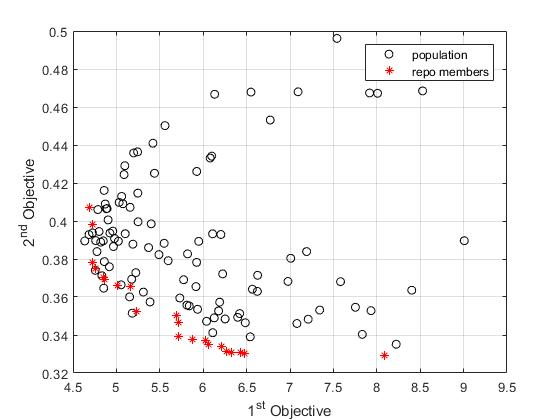
\includegraphics[scale=.6]{Fig/repo_members.jpg}
\caption{Particles stored in external repository approximate the Pareto front. \textcolor{red}{This fig does not appear for some reason.}}
\label{fig:repo_members}
\end{figure}

Using the concept of Pareto optimality, we demonstrate the impact of applying kernel functions in this spatial reshaping problem by comparing the \textcolor{blue}{Pareto front of the optimization problem obtained by using MOPSO} for two different scenarios including i) the optimized coefficients for the original data sample, (i.e. a linear identity function) and ii) the transformed samples under polynomial kernel whose coefficients are optimized using MOPSO. Therefore, we first optimize the coefficients of the third-order polynomial kernel function, as formulated in Eq.\ref{eq5} and then optimize the coefficients of linear features in the origin feature space. The purpose of this comparison is to investigate whether or not the resulting objective functions are fundamentally improved by incorporating nonlinear terms into the feature vectors through the proposed polynomial function.  %A two-dimension curve formed by repository members t will be drawn with two objective functions.

%This mapping by kernel method can be accounted as the input space reshaping, namely, new input sample space is produced using non-linear kernel bending feature space in order for a higher space symmetry. Reshaping result as indicated in diagram 4-6 can be obtained through testing the reshaping algorithm with test data and quadratic polynomial. More specifically, we can regard this kernel method as a mapping from two-dimension space   to three-dimension space. Because the data visualization is very important in the test, we don’t adopt polynomial kernel of higher degree.

As shown in Fig. \ref{fig:pareto_compare}, the estimated Pareto front of the nonlinear model using the polynomial kernel dominates the Pareto front of the original linear model. This result is expected since the transformed samples exhibit a higher degree of freedom by adding new dimension to the data in the feature space through the nonlinear mapping. 
A higher degree of freedom enables the MOPSO algorithm to tune the optimization parameters and find better solutions than the best solutions achievable by the original data samples. In other words, the kernel method combined with multi-objective particle swarm optimization algorithm can improve the spatial structure of the clusters quantified by the two objective functions.

%\subsubsection{Pareto Front}
\begin{figure}[t]
\centering
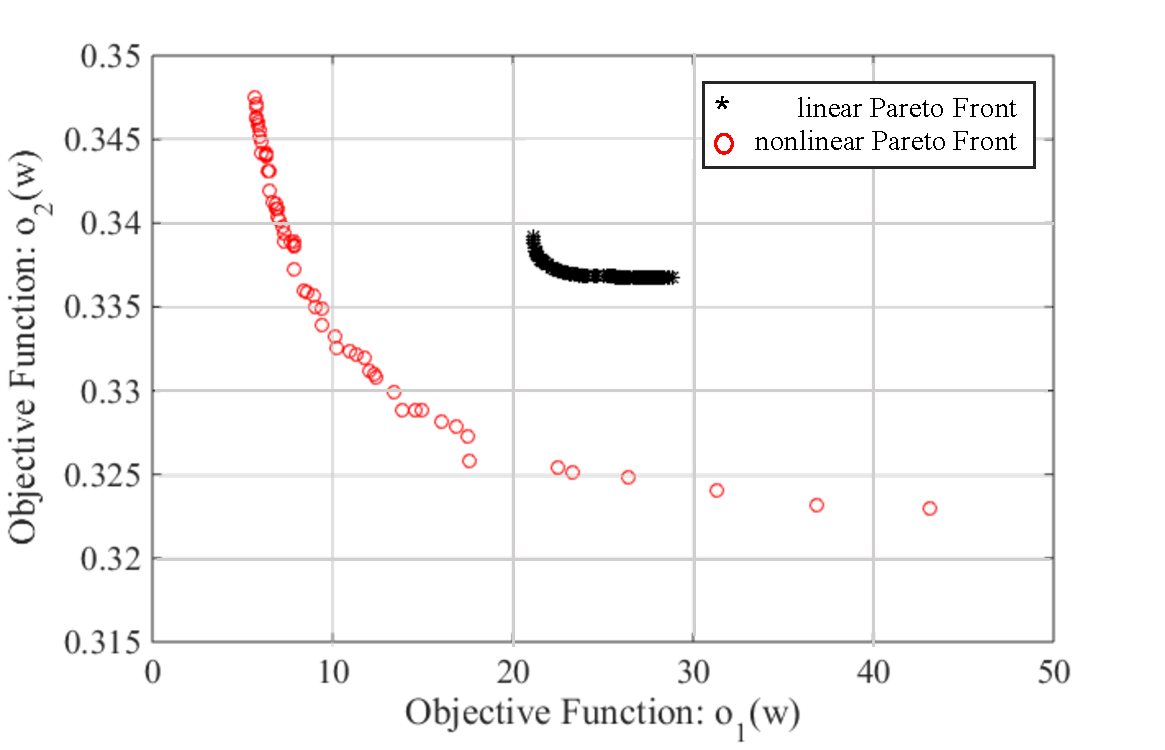
\includegraphics[scale=.6]{Fig/pareto_compare.pdf}
\caption{The \textit{Pareto front} of the results of MOPSO is significantly shifted when using the transformed feature vectors. This improvement is due to the increase in the degree of freedom provided by additional non-linear dimensions added to the samples.}
\label{fig:pareto_compare}
\end{figure}

\section{Experimental Results}\label{sec:result1}

%This section will introduce the experimental result of the aforementioned kernel-based method on test set DS2 of MITDB to show the performance. 
As mentioned in Section. 2.3 \textcolor{red}{better to use refs to make sure section numbers are correct.}, a cardiac segment is represented by an 8-dimensional vector $\mathbf{x}=[x_1,x_2,\dots,x_8]$ after the feature extraction and the PCA-based dimension reduction stages. %In order to reduce the complexity,  we firstly map the original 22-dimensional feature vectors, representing cardiac segments, into an 8-dimensional vectors $\mathbf{x}_{8 \times 1}$ using Principal Component Analysis (PCA). 
To specify the nonlinear transformation in (\ref{eq:z}), a polynomial function of order $3$ is applied to the feature vectors.
The resulting transformed vectors $[x_1,x_2,\dots,x_8,x_1^2,x_2^2,\dots,x_8^2,x_1^3,x_2^3,\dots,x_8^3,x_1x_2,....x_6x_7x_8]$ include $XXX$ terms, 8 of which are the original features. 
This high dimension may cause the classifier to trap into the overfitting problem. It also significantly increases the computational complexity of the algorithm. To solve these issues, we discard some of the induced terms and include only 8 square terms $x_i^2$, 8 cubic terms $x_i^3$, and 8 cross terms of power two $x_ix_j$ and 8 cross terms of power three $x_i x_j^2$. We randomly choose these terms after discarding the redundant cross terms. Therefore, the mapped vectors $\mathbf{z}_{32 \times 1}$ include a total of $32$ terms as follows:

\begin{align}
\label{eq:8-32}
\mathbf{z}&=\{x_i^2|i=1,2\dots 8\}\cup\{x_i^3|i=1,2\dots 8\} \cup\\
\nonumber
& \{x_ix_j|i,j=1,2\dots 8,i\neq j\} \cup  \{  x_i^2x_j | i,j=1,2\dots 8,i\neq j \}
\end{align}

The performance of the aforementioned kernel-based method is tested on DS2 excluding record 232, for this record has only 7 normal samples $y_k=N$. In total, 21 records are tested.

Table \ref{table:result1} shows the performance of the proposed method in classifying ECG signal segments. In order to evaluate the consistency as well as the general classification classification results over all recordings, the median, interquartile range (IQR), mean and standard deviation of accuracy (AC), sensitivity (SE) and specificity (SP) are presented. The results are promising and the median of the classification accuracy for all classes are in the range of $88\%-99\%$. Sensitivity and specificity of the proposed method exhibit similar ranges. The mean accuracy is at least $86\%$ excluding class $V$. Therefore, this system is not likely to miss an important alarm or to report false alarms. 

\begin{table}[t]
	\caption{Classification results of the proposed method.}
	\centering
	\begin{tabular}{|c|c|c|c|c|}
		\hline
		Class N & median(\%) & IQR(\%) & mean(\%)& std (\%) \\ 
		\hline 
		AC & 94.8& 19.52 & 86.62 & 18.55\\ 
		\hline 
		SE & 97.21  & 17.36 & 87.47 &19.26 \\ 
		\hline 
		class V & median(\%) & IQR(\%) & mean(\%)& std (\%) \\ 
		\hline 
		AC & 86.11 & 27.54 & 76.41 & 22.81 \\ 
		\hline 
		SP & 99.71 & 11.22 & 90.18 & 18.52 \\ 
		\hline 
		class S & median(\%) & IQR(\%) & mean(\%)& std (\%)\\ 
		\hline 
		AC & 99.28 & 2.24& 98.29&2.57 \\ 
		\hline 
		SP & 99.64& 22.17& 97.56 & 6.06\\ 
		\hline 
		class F & median(\%) & IQR(\%) & mean(\%)& std (\%) \\ 
		\hline 
		AC & 97.91 & 8.2&93.85&7.84\\ 
		\hline 
		SP & 100.00 & 0.03&99.12&3.6\\ 
		\hline 
	\end{tabular} 
	\label{table:result1}
\end{table}

%%%%%%%%%%%%555

More importantly, the predictive capability of the proposed method is worthy of evaluating, since it is unique feature provided by the proposed system. In order to quantify the posterior probability of observing an abnormal signal after a preceding yellow alarm of similar type in (\ref{eq:personal_discrim}), the number of predicted samples are counted as formulated in Eq \ref{eq:proab}:

\begin{align}
\nonumber 
&P(\hat{y}_{k+i}=X_r|\hat{y}_{k}=X_y)=\frac{\text{\# of $y_{k+i}=X$ after $\hat{y}_k=X_y$}}{\text{\# of true alarms after $\hat{y}_k=X_y$}} \\
&P(\hat{y}_{k+i}=X_r)=\frac{\text{\# of true alarm of type $X$ ($y_{k}=X$)}}{\text{\# of all true alarms}} 
\label{eq:proab}
\end{align}

The summary of results for all 21 test records is presented in Table. \ref{table:pred}. The values provided under the column \textit{Probability of next abnormality (\%)} in Table. \ref{table:pred} present the probability of having a subsequent true abnormality of all types after observing a yellow alarm of all types along with the prior probability of observing a certain type regardless of the preceding yellow alarm in the very last column. %The last 4 columns of the Table. \ref{table:pred} show the confusion matrix of the probability of having a subsequent true abnormality of all types after observing a yellow alarm of all types. It's compared with the probability of having the same type of abnormality after a secondary abnormality of its own type. 
These results confirm the predictive capability of yellow alarms as well as the scientific fact that yellow alarm are indicative of upcoming red alarms. This conjecture supported by the fact that at least some of the heart problems develop over time, although the symptoms may appear suddenly. 
 
For instance, the prior probability of observing a sample segment with abnormal types $V$, $S$, and $F$ is respectively $\frac{96}{96+29+18}=67\%$, $\frac{29}{96+29+18}=20\%$ and $\frac{18}{96+29+18}=13\%$, based on their relative frequencies in the dataset. However, the corresponding posterior probabilities after observing a yellow alarm of type $Vp$ are respectively $\frac{38}{38+11+2}=75\%$, $\frac{11}{38+11+2}=21\%$ and $\frac{2}{38+11+2}=4\%$. This means that the probability of observing a real abnormal segment of type $V$ is $75\%-67\%=8\%$ higher than its prior probability. The same trend holds for other yellow alarms as well. The results suggest a more in-depth study of the concept of yellow alarms for heart monitoring. 
We conclude this section by stating that a new methodology provided in Chapter 4 to optimize the nonlinear transformation using an analytical approach, which significantly reduces the computational cost.

\begin{table}
	\caption{Predictive power of yellow alarms: A yellow alarm increases the chance of observing a red alarm of the same type.}
	\centering
	%\resizebox{\textwidth}{!}{
	\begin{tabular}{|m{6em}| m{2em}| m{2em}| m{2em} |m{2em}| m{2em}| m{2em}| m{2em}| m{2em}|}
		\hline
		& \multicolumn{3}{p{6em}}{Count numbers of subsequent abnormality}& &\multicolumn{3}{p{6em}}{Probability of subsequent abnormality (\%)}  & \\ 
		\hline 
		secondary abnormalities & $V_y$ & $S_y$ & $F_y$ & Total & $V_y$ & $S_y$ & $F_y$ & Total \\ 
		\hline 
		True V & 38 & 23 & 35& 96 & 75 & 75 & 61 & 67 \\ 
		\hline 
		True S & 11 & 10 & 8 & 29 & 21 & 29 & 14& 20 \\ 
		\hline 
		True F & 2 & 2 & 14 & 18 & 4 & 6 & 25 & 13 \\ 
		%		\hline 
		%		Total & 4 & 20 & 0 & 24 & 100 & 100 & 100 & 100\\
		\hline 
	\end{tabular}%} 
	\label{table:pred}
\end{table}


\section{Summary of contributions} 
\textcolor{red}{It is usual to have a summary of contributions at the end of each chapter. Conclusions and future works should be a separate section [bit 2 or 3 pages is sufficient.}

\textcolor{red}{Part of the text here is the repetition of the text before revision. reword this section and provide a list of contributions and concluding remarks here. The overall conclusions should be provided in a separate section}
\textcolor{blue}{In this chapter, we proposed a novel method which combines kernel-based nonlinear transformation with MOPSO optimization method. Inspired by the concept of kernel method and the loss function utilized in SVM, we implement the method with a weighted combination of base nonlinear kernels to reshape the input feature space by mapping it to a high-dimensional space. The coefficients of kernels are optimized according to two conditions, namely, maximum separation between cluster and maximum cosine similarities between abnormal clusters.\\
Result shows that approximated Pareto front produced by kernel method in the objective function space is apparently optimal to the one which is produced by the linear combinations of original features. The results verify that the proposed method has a classification accuracy in the range of $88\%-99\%$ for different ECG records in the test set of MIT-BIH database.\\
Above all, the proposed algorithm demonstrates the potential of providing detailed information about the sample deviations, which indicate the upcoming abnormal sample types. The predictive capacities of the system is verified with ECG signal, but this method is general and not bound to this application. If a biomedical signal has one base class (i.e. normal state) and several abnormal states, the proposed method can be implemented to predict upcoming abnormal types.}
  

\fbox{\textcolor{red}{Revised up to here}}
 %\chapter{\textit{Kernels}-Based Nonlinear Spatial Transformation}\label{ch:spheremapping}
\section{Introduction}

As discussed in Chapter 2, the main objective of the personalized classifier is to reassess the normal samples to identify deviation of seemingly normal samples into any of abnormality types. \textcolor{blue}{The original geometry of clusters in the feature space $\Omega^d$ depends on the choice of features implied by the feature extraction and feature selection stages $g()$}. We noticed that with the resulting features (in this work), the clustering geometry does no exhibit the necessary symmetric property and thus leads to a poor performance and even failure in predicting subsequent abnormalities. 
Therefore, an optimization method based on spatial transformation is proposed to solve this issue. More specifically, we propose a method to reshape the clusters such that 
 \begin{itemize}
\item The abnormal classes surround the normal class; 
\item A maximal separation among the abnormal classes are achieved; 
\item The angles between the vectors connecting the centroid of normal cluster to different abnormal clusters are equalized. 
\end{itemize}

These properties can be achieved through imposing the following conditions:  
 \begin{itemize}
     %\item Vectors pointing from normal centroid to different abnormal clusters centroids has no overlapping or cross with each other.
     \item Vectors pointing from the normal centroid to different abnormal clusters centroids present maximum mutual cosine distances.
     \item The overlapping parts among all clusters are minimized.
 \end{itemize}

% maximizing the minimum of the angles between the aforementioned vectors from the normal cluster centroid to abnormal cluster centroids. 


Given that the clusters in original feature space do not meet these symmetric properties, developing a spatial transformation is unavoidable. In this chapter, a \textit{kernel}-based nonlinear spatial transformation is proposed to reshape the feature space to reach the above-mentioned required symmetric properties. 
%Here, we assume in this chapter that new feature space obtained by non-linear reshaping is noted as $\Phi^{d'}$. 
\textcolor{blue}{This reshaping process is part of the \textcolor{blue}{\textit{personalized classification}} stage (as shown in Fig.\ref{fig:flow}) of the ECG classification system as described in chapter 2. The nonlinear mapping projects the corresponding feature vector of each sample $\mathbf{x}_k$  in the original space $\Omega^d$ onto a new vector $\mathbf{z}_k$ in a higher dimensional space denoted by $\Omega^{d^\prime}$.  This is achieved using a nonlinear mapping function $\Phi^{d'}:\Omega^{d} \rightarrow \Omega^{d^\prime}$. The resulting vectors are used by the personalized classifier to identify the minor yellow alarm type out of $\{\mathcal{N},\mathcal{S},\mathcal{V},\mathcal{F}\}$.}
\textcolor{red}{
The original text was ambiguous. Firstly, set and cluster shapes can be viewed differently, sets are not changes under the transformation although cluster geometry changes. Therefore, since we already used $\mathcal{N},...$ to represent clusters in the original space, you can use $\mathcal{N'},....$ for the transformed clusters, unless you mean a set (not a cluster). In this case, sets do not changes under the transformation, and you can omit the definition $\Phi^{d'}=\{\mathcal{N},\mathcal{S},\mathcal{V},\mathcal{F}\}$ to avoid ambiguity.
Secondly, you need to distinguish between two functions, one simply maps the vector in original space into a new space, and the second one processes the transformed vector and maps it to a yellow alarm. It is not clear in the text.}

%  which can be considered as the union of subspaces for transferred types: %$\Phi^{d'}=\{\mathcal{N},\mathcal{S},\mathcal{V},\mathcal{F}\}$, where $d'>d$. 
  

\section{\textit{Kernel} Method}

Kernel method has been widely used in machine learning algorithms. For instance, it is the integral part of nonlinear Support Vector Machine (SVM), which has been utilized in numerous applications recently\cite{shawe2004kernel}. Nonlinear kernel methods can efficiently improve the classification performance when there exists a nonlinear relationship between the input and output variables. Because of the complexity and diversity of feature vectors used in ECG analysis, the assumption of nonlinear relationship is considered valid in this work. Therefore, incorporating nonlinear kernel methods in the ECG analysis system, can be beneficial.

In kernel SVM, the nonlinearities are introduced to the model through a kernel function, which implicitly maps data points $\mathbf{x_i} \in \mathcal{X}$ in the input space $\Omega$ into a Hilbert space $\Phi$ via a nonlinear function $\Psi()$\cite{aronszajn1950theory}. Then, the algorithm minimizes the expected error $E[L(y,f(x)]$ between the true labels $y$ and the predicted values $f(x)$ for samples in a training dataset, by finding an optimal classification function $f$, which also depend on the choice of $\Psi()$. Here, $L()$ is an arbitrary loss function, and a popular choice is the least squared errors $\sum\limits_{x_i \in \mathcal{X}} (y_i-f(x_i))^2$ \cite{scholkopf1999advances}. \textcolor{red}{Other choices for loss function include Hindge loss, absolute loss, hit and miss loss, etc [REF]}.

If there are $m$ observations in the input space, we use notation $\mathbb{N}$ for index set ${1:m}$. Based on the input space $\mathbf{x_i}\in \Omega (i\in \mathbb{N})$ and classification mapping function $f$, the optimization problem can be written as:
\textcolor{red}{better to use $n$ instead of $m$ if it does not conflict with other definitions.}
\begin{align}
    \text{minimize}~\frac{1}{m}\sum_{i\in \mathbb{N}}L(y_i,f(\mathbf{x_i})) + \gamma||f||^2,
    \label{eq:kernel}
\end{align}

where $||f||^2$ is the squared norm of $f$ \textcolor{red}{here f is a function and norm is defined for vectors. So add one or two sentences how to calculate it. I think for instance you mean the norm of coefficients of a polynomial function here.}% on Hilbert space $H_K$. 
and the positive constant $\gamma$, also known as the regularization parameter, controls the balance between training error and the model complexity (smoothness).



%For example, if $H_K$ is the Hilbert space of linear functions, the $f$ can be written as $f=w' x,~w\in\mathbb{R}^d$. Therefore, the loss function can be written as:

%\begin{align}
%    \frac{1}{m}\sum_{i\in \mathbb{N}}L(y_i,w'\mathbf{x_i}) + \gamma w'w
%    \label{eq:kernel}
%\end{align}

%Positive constant $\gamma$, also known as the regularization parameter, controls the balance between training error and the model complexity (smoothness). 
When optimizing the above objective function, SVM only requires the inner products of the transformed features $\Psi(\mathbf{x})$ in the Hilbert Space $\Phi$. Therefore, a kernel defined as $k(\mathbf{x_i},\mathbf{x_j}) = \Psi(\mathbf{x_i})^T\Psi(\mathbf{x_j})$ can efficiently substitute the inner product calculation and induces the necessary nonlinearities into the model\cite{evgeniou2000regularization}.

%In SVM and other machine learning models, nonlinear kernel methods are implemented with different loss functions \cite{evgeniou2000regularization}. But in more general conditions, the solution to Eq.\ref{eq:kernel} can be written as follows: 

%\begin{align}
%    f(x)=\sum_{i\in \mathbb{N}}c_i K(\mathbf{x_i},\mathbf{x} )
%    \label{eq:kernel2}
%\end{align}

%where ${c_i: i \in \mathbb{N}}$ is a set of real number, $K$ is a kernel such as a polynomial kernel of order $r$: $K(x,t)=(x't)^r,~x,t\in \mathbb{R}^d$.

%For any kernel $K$, it has the following properties: i) for $\mathbf{x} \in \Omega$, $K(\mathbf{x},\cdot)\in H_K$; ii) for $f\in H_K$, $<f,K(\mathbf{x},\cdot)>_K = f(\mathbf{x})$, where $<\cdot,\cdot>_K$ represents the inner product of $H_K$\cite{aronszajn1950theory}.

%A kernel is usually defined base on feature mapping concept, in this work we define this mapping function as $\Psi:\Omega^d\to \Phi^{d'}$ %where $\Psi^{d'}$ is Hilbert space and $<,>_{\Phi}$  represents inner product. 
%Therefore, Eq.\ref{eq:kernel2} can be also written as:

%\begin{align}
%    f(x) = \sum_{i\in \mathbb{N}}c_i \Psi(x_i,x)
%\end{align}



Different \textit{kernels} represent different nonlinear mapping functions. For machine learning models, the selection of kernel plays a crucial role. Therefore is no straightforward method to choose the best kernel and it is typically chosen by try and error and other heuristic model selection methods. An effective kernel function generally needs to satisfy Mercer conditions, so that the inner products can be replaced by kernel functions, as used in SVM \cite{cristianini2000introduction}. 
%This means the matrix defined by function $\Psi(x_j,x)$ is symmetric positive semi-definite. In general, the selection of kernel function depends on all observations in input space. 
An exhaustive search for all possible kernels is a computationally expensive and unrealistic task\cite{chapelle1999support}. A more efficient way to resolve this issue would be to search for an optimally weighted combination of a set of base kernels, such as polynomial kernel function and Gaussian kernel function\cite{lanckriet2002robust}. This method has been proven to be robust and efficient since the base kernels satisfy Mercer’s condition individually and it can be consistent with different datasets\cite{jebara2004multi}.
%However, in effect, kernel functions with simple expression, such as polynomial kernel function, Gaussian kernel function and exponential kernel function are usually preferred than complicated kernel function for its simplicity and consistency. 


Polynomial kernel is usually applied on normalized data for its explicit expression and steady performance. However, the degree of freedom in defining a polynomial kernel is relatively high, which requires tuning a large number of parameters. \textcolor{red}{In fact this statement is not so relevant here. Note that a polynomial kernel of order $p$ can be defined as $(1+v^Tw)^p=(1+v_1w_1+v_2w_2+...)^p$, which has only one free parameter $p$ and all coefficients are automatically determined. However, we are going to use a polynomial function of order $p$, (i.e. $f(v)=1+\alpha_1 v_1+\alpha_2 v_2+...+ \alpha_i v_1^2 + \alpha_j v_1v_2+... \alpha_k v_N^p$) which obviously required tuning too many free coefficients $\alpha_i$.}

Gaussian kernel function \textcolor{red}{denoted by XXX for vectors v and w} is a very classic robust radial function, which has shown a string robustness in the case of noisy datasets [REF XXX]. However, it is equivalent to the inner product of samples after projecting into an infinite dimensional space; therefore it is difficult to visualize the projected observations $\Psi(\mathbf{x})$ and interpret the results. %Moreover its performance is greatly affected by parameter selection.

Considering the above-mentioned facts, in this work, the polynomial kernel is selected for the purpose of validating the proposed method and interpreting the effect of an optimized nonlinear kernel method on feature space reshaping. However, the proposed methodology is general and applicable to other nonlinear kernels.

The mapping function, which is a weighted combination of polynomial kernels can be explicitly written in the following format:

\begin{align}
\mathbf{z}_k
=\mathbf{\Psi_{w}} (\mathbf{x}_k) = 
\begin{bmatrix}
w_{1}  \\
w_{2}   \\
\vdots \\
w_{d^\prime} 
\end{bmatrix}
\circ
\begin{bmatrix}
\psi_1(\mathbf{x}_k)\\
\psi_2(\mathbf{x}_k)\\
\vdots\\
\psi_{d^\prime}(\mathbf{x}_k)
\end{bmatrix} \color{red}{,}
\label{eq:z}
\end{align}
where $\mathbf{w}$ is the vector of \textcolor{blue}{normalized} coefficients \textcolor{red}{do we have $||w||=1$}. Instead of selecting kernel, %The example above shows that regardless the selection of kernel function, parameter optimization will play a critical role. For instance, in this work, 
the process of spatial geometry optimization is accomplished by adjusting the coefficients of fixed polynomial basis functions $\psi()$. Since the number of free parameters increases exponentially with the order of polynomial function, an exhaustive search is not practical for parameter optimization. Therefore, it is necessary to implement a heuristic optimization algorithm, in which parameters are obtained by maximizing or minimizing an objective function. More specifically, the nonlinear reshaping module in this chapter aims to adjust mapping coefficients  $\mathbf{w} = [w_1,w_2,\dots w_d]^T$ to achieve the ideal symmetric geometry in the reshaped feature space while maintaining the maximal separation between clusters.


\section{Multiobjective Optimization}

\subsection{Objective Functions}

To elucidate the details of the optimization problem, here we consider an illustrative example, where the original feature space is a 2-dimensional space $\Omega^2$. \textcolor{red}{This is not necessarily true, since you can choose any order of power even for a 2-D input vector. Therefore, the mapping base kernel may adopt a second-order polynomial function as follows:}
We also assume for simplicity that the order of the polynomial function is 2. Therefore, we have:

\begin{align}
\nonumber
&\mathbf{x}=[x_1~ x_2]^T,~~ \mathbf{w}=[w_1~ w_2~ \dots~ w_5]^T,~~d=2, ~~d^\prime=5,\\
&\psi_1(\mathbf{x})=x_1, \psi_2(\mathbf{x})=x_2, \psi_3(\mathbf{x})=x_1^2, \psi_4(\mathbf{x})=x_2^2, \psi_5(\mathbf{x})=x_1x_2.
\label{eq5}
\end{align}
\textcolor{red}{when you start the sentence with ``where'', it means that the equation is connected to the following sentence, so it is better to add a comma to the end of equation. Otherwise, add dot ``.''. I fixed some, but make sure that you do it consistently.}

\fbox{\textcolor{red}{Revised up to here}}

Using similar concept to the loss function in the standard kernel SVM, the following objective functions can be used to represent the symmetric structure to be obtained:

\begin{align}
\label{eq:obj}
&o_1(\mathbf{w}) = \frac{1}{\underset{c,d=2,\dots,p \text{ and } c\neq d }{\min}\{d(\mathbf{v}_{\mathcal{X}_c},\mathbf{v}_{\mathcal{X}_d})\}} \\ %|a,b=1,2\dots k;a\neq b)
\nonumber 
&o_2(\mathbf{w}) = \frac{SW}{SB}=\frac{\sum_{c=1}^{C}  \sum_{\mathbf{z} \in \mathcal{X}_c}   (\mathbf{z}-\mathbf{c}_{\mathcal{X}_c})^T(\mathbf{z}-\mathbf{c}_{\mathcal{X}_c})}{\sum_{c=1}^{C}\sum_{d=1, d\neq c}^{C}  (\mathbf{c}_{\mathcal{X}_c}-\mathbf{c}_{\mathcal{X}_d})^T(\mathbf{c}_{\mathcal{X}_c}-\mathbf{c}_{\mathcal{X}_d}) }
\end{align}

The maximization of pairwise cosine distance between vectors $\mathbf{v}_{\mathcal{X}_{c,d}}$, which connect the centroid of the normal cluster to centroids of abnormal clusters $\mathcal{X}_c$, can be obtained by minimizing $o_1(\mathbf{w})$. In fact, this objective functions is deduced from discrimination function of personal classifier in Eq.\ref{eq:personal_discrim}. Cosine distance is defined by Eq.\ref{eq:cosine} and the calculation of $\mathbf{v}_{\mathcal{X}_{c,d}}$ is as follows: %In the formula, vectors used to measure symmetry is defined by abnormal sample sets in training set DS1 and the personal normal cluster as follows:

\begin{align}
\mathbf{v}_{\mathcal{X}_i} = \mathbf{c}^k_N -  \mathbf{c}_{\mathcal{X}_i}
\end{align}

Since, for some patients, the total number of a certain type of abnormal samples are very limited, abnormal samples in trainign set DS1 are utilized in calculating the two objective functions. In Eq.\ref{eq:obj}, the abnormal cluster centroids are calculated using abnormal sample sets in training set DS1, while the normal cluster centroid is defined by the personal normal cluster. 

On the other hand, $o_2(\mathbf{w})$ represents the ratio of within-cluster variance to between-cluster variance and consequently controls the separation between clusters. By minimizing $o_1(\mathbf{w})$ and $o_2(\mathbf{w})$ jointly, the algorithm eliminates the ambiguity while using Eq.\ref{eq:personal_discrim} to discriminate latent abnormal state and improves the predictive capability.

\subsection{Multiobjective Particle Swarm Optimization}

We noticed that $o_1(\mathbf{w}) $ and $o_2(\mathbf{w})$ are not necessarily independent to each other. Thus, the optimization problem defined above is equivalent to joint minimization of $o_1(\mathbf{w}) $ and $o_2(\mathbf{w})$ subject to a constraint condition: $|w|_2=1$. Since this is a non-convex multiobjective optimization problem, closed form solution as well as the optimization methods for convex function are not adopted in this method. In this work, we utilize Multiobjective Particle Swarm Optimization (MOPSO) algorithm to solve this optimization problem and obtain the optimal coefficients.

Particle Swarm Optimization (PSO) has the advantage of fast-converging, heuristic searching and easy implementation\cite{coello2002mopso, alvarez2005mopso}. Therefore, researchers have been investigating in extending PSO to multiobjective optimization problems. In the framework of MOPSO, the goal is to solve the typical Pareto optimization problem based on the algorithm in PSO. In other words, it aims at solving an optimization problem with two or more conflicting objective functions by approximating the Pareto front. 

\subsubsection{Pareto Front}

In order to compare different set of coefficient in this opmization problem, the concept of Pareto front is briefly introduced in this section. For a multiobjective optimization problem with two objective function, if a solution $\mathbf{w}^1$ is said to \textit{dominate} another $\mathbf{w}^2$ when the following two conditions are satisfied:
\begin{enumerate}
    \item $o_1(\mathbf{w}^1) \leq  o_1(\mathbf{w}^2)$ and $o_2(\mathbf{w}^1) \leq  o_2(\mathbf{w}^2)$ 
    \item $o_1(\mathbf{w}^1) <  o_1(\mathbf{w}^2)$ or $o_2(\mathbf{w}^1) < o_2(\mathbf{w}^2)$ 
\end{enumerate}

If a solution is not dominated by any other solutions in the searching space, then this solution is an \textit{optimal} solution for this problem. A Pareto front is defined by the set of Pareto optimal solutions. However, in non-convex optimization, the Pareto front can not be represented explicitly by a deterministic function. Therefore, the majority of algorithms use heuristic searching algorithms to approximate the Pareto front\cite{coello2002mopso}.

\subsubsection{MOPSO}

Among all the MOPSO algorithms in the literature, the algorithm proposed by Coello Coello and Lechug presents a better performance and lower computational complexity than most of the other MOPSO algortihms\cite{coello2002mopso}. Therefore, this algorithm implemented to solve the optimization problem in this work. One characteristic property of this algorithm is the external repository, in which all Pareto optimal particles for every swarm is recorded for each iteration. The solution represented by repository members are stored and used as an optimal approximation of the Pareto front because they converge to the actual Pareto front as proved in \cite{coello2002mopso}. Fig.\ref{fig:repo_members}, which is generated by jointly minimizing $o_1(\mathbf{w}) $ and $o_2(\mathbf{w})$, demonstrates the repository members are Pareto optimal than other particles and they converge to a uniform Pareto front.

\begin{figure}[t]
\centering
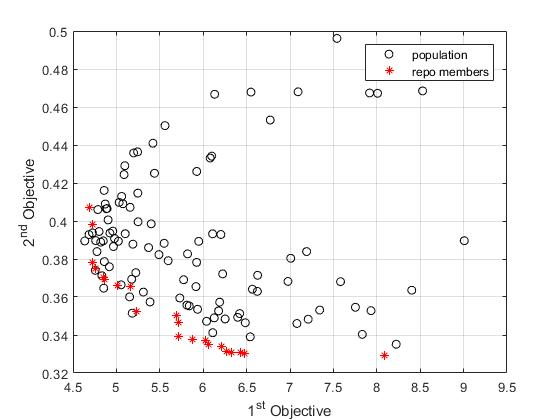
\includegraphics[scale=.6]{Fig/repo_members.jpg}
\caption{Particles stored in external repository approximate the Pareto front}
\label{fig:repo_members}
\end{figure}

With the concept of Pareto optimal, we further demonstrate the impact of applying kernel functions in this spatial reshaping problem by comparing the optimal solutions for coefficients of linear function combination and those for coefficients of polynomial kernel functions. Therefore, we first optimize the coefficients of third-order polynomial kernel functions, as formulated in Eq.\ref{eq5} and then optimize coefficients of linear features in origin feature space. The purpose is to verify if the objective functions can be fundamentally better optimized by introducing nonlinearities into the model. %A two-dimension curve formed by repository members t will be drawn with two objective functions.

%This mapping by kernel method can be accounted as the input space reshaping, namely, new input sample space is produced using non-linear kernel bending feature space in order for a higher space symmetry. Reshaping result as indicated in diagram 4-6 can be obtained through testing the reshaping algorithm with test data and quadratic polynomial. More specifically, we can regard this kernel method as a mapping from two-dimension space   to three-dimension space. Because the data visualization is very important in the test, we don’t adopt polynomial kernel of higher degree.

As shown in Fig. \ref{fig:pareto_compare}, the estimated Pareto front of the nonlinear model using polynomial kernel obviously dominates the Pareto front of linear model consist. The result shows that optimization with nonlinear kernel functions possess a higher degree of freedom and is able to find optimal solutions than the best solutions by linear combination. In other words, kernel method combined with multiobjective particle swarm optimization algorithm can improve the spatial structure of clusters according to the two objective functions.

%\subsubsection{Pareto Front}
\begin{figure}[t]
\centering
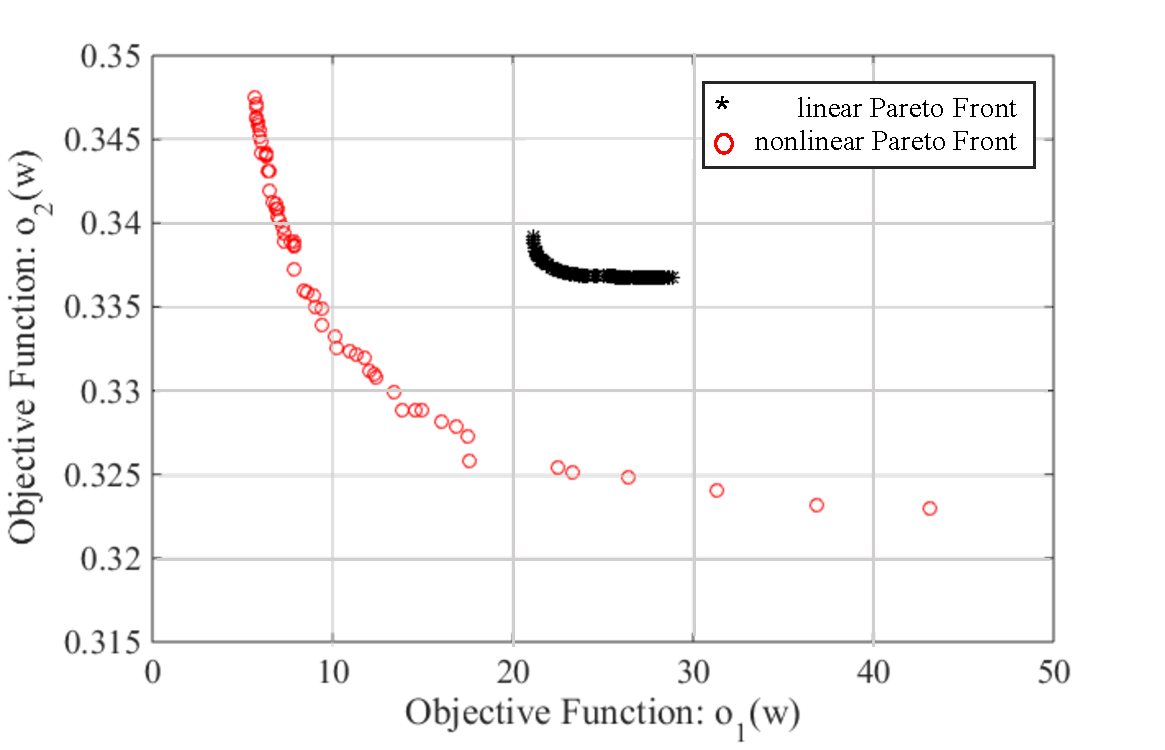
\includegraphics[scale=.6]{Fig/pareto_compare.pdf}
\caption{Increase of degree of freedom in optimization is proved by comparing the Pareto fronts generated by linear and nonlinear basis function}
\label{fig:pareto_compare}
\end{figure}

\section{Experimental Results}\label{sec:result1}

%This section will introduce the experimental result of the aforementioned kernel-based method on test set DS2 of MITDB to show the performance. 
As mentioned in Section. 2.3, a cardiac segment is represented by an 8-dimensional vectors after feature extraction and PCA. %In order to reduce the complexity,  we firstly map the original 22-dimensional feature vectors, representing cardiac segments, into an 8-dimensional vectors $\mathbf{x}_{8 \times 1}$ using Principal Component Analysis (PCA). 
To specify the nonlinear transformation in (\ref{eq:z}), the polynomial functions of order $3$ is applied on the feature vectors. Moreover, taking the overfitting problem in high-dimensional space and computational cost into account, only $32$ terms, which include 8 square terms $x_i^2$, 8 cubic terms $x_i^3$, 8 cross terms $x_ix_j$ of second order and 8 cross terms $x_i x_j^2$ of third order, are retained by randomly discard the redundant cross terms. Therefore, the mapped vectors $\mathbf{z}_{32 \times 1}$ include a total of $32$ terms as follows.

\begin{align}
\label{eq:8-32}
\mathbf{z}&=\{x_i^2|i=1,2\dots 8\}\cup\{x_i^3|i=1,2\dots 8\} \cup\\
\nonumber
& \{x_ix_j|i,j=1,2\dots 8,i\neq j\} \cup  \{  x_i^2x_j | i,j=1,2\dots 8,i\neq j \}
\end{align}

The performance of the aforementioned kernel-based method is tested on DS2 excluding record 232, for this record has only 7 normal samples $y_k=N$. In total, 21 records are tested.

Table \ref{table:result1} shows the performance of the proposed method in classifying ECG signal segments. In order to evaluate the consistency and general classification classification results over all recordings, the median, interquartile range (IQR), mean and standard deviation of accuracy (AC), sensitivity (SE) and specificity (SP) are presented as evaluation metrics. The results are promising and the median of accuracy for all classes are in the range of $88\%-99\%$. Sensitivity and specificity of the proposed method exhibits similar ranges. The mean accuracy is at least $86\%$ excluding class $V$. Therefore, this system is not likely to miss an important alarm or to report false alarms. 

\begin{table}[t]
	\caption{Classification results of the proposed method.}
	\centering
	\begin{tabular}{|c|c|c|c|c|}
		\hline
		Class N & median(\%) & IQR(\%) & mean(\%)& std (\%) \\ 
		\hline 
		AC & 94.8& 19.52 & 86.62 & 18.55\\ 
		\hline 
		SE & 97.21  & 17.36 & 87.47 &19.26 \\ 
		\hline 
		class V & median(\%) & IQR(\%) & mean(\%)& std (\%) \\ 
		\hline 
		AC & 86.11 & 27.54 & 76.41 & 22.81 \\ 
		\hline 
		SP & 99.71 & 11.22 & 90.18 & 18.52 \\ 
		\hline 
		class S & median(\%) & IQR(\%) & mean(\%)& std (\%)\\ 
		\hline 
		AC & 99.28 & 2.24& 98.29&2.57 \\ 
		\hline 
		SP & 99.64& 22.17& 97.56 & 6.06\\ 
		\hline 
		class F & median(\%) & IQR(\%) & mean(\%)& std (\%) \\ 
		\hline 
		AC & 97.91 & 8.2&93.85&7.84\\ 
		\hline 
		SP & 100.00 & 0.03&99.12&3.6\\ 
		\hline 
	\end{tabular} 
	\label{table:result1}
\end{table}

%%%%%%%%%%%%555

More importantly, the predictive capability of the proposed method is worthy of evaluating exclusively for it is the featuring specialty of the proposed system. In order to quantify the posterior probability of observing an abnormal signal after a preceding yellow alarm of similar type in (\ref{eq:personal_discrim}), the number of predicted samples are counted as formulated in Eq \ref{eq:proab}:

\begin{align}
\nonumber 
&P(\hat{y}_{k+i}=X_r|\hat{y}_{k}=X_y)=\frac{\text{\# of $y_{k+i}=X$ after $\hat{y}_k=X_y$}}{\text{\# of true alarms after $\hat{y}_k=X_y$}} \\
&P(\hat{y}_{k+i}=X_r)=\frac{\text{\# of true alarm of type $X$ ($y_{k}=X$)}}{\text{\# of all true alarms}} 
\label{eq:proab}
\end{align}

The summary of results for all 21 test records is presented in Table. \ref{table:pred}. The subsection \textit{Probability of next abnormality (\%)} in Table. \ref{table:pred} shows the confusion matrix of the probability of having a subsequent true abnormality of all types after observing a yellow alarm of all types along with the prior probability of observing a certain type of abnormal sample in the very last column. %The last 4 columns of the Table. \ref{table:pred} show the confusion matrix of the probability of having a subsequent true abnormality of all types after observing a yellow alarm of all types. It's compared with the probability of having the same type of abnormality after a secondary abnormality of its own type. 

These results validate the predictive capability of yellow alarms. 
For instance, the prior probability of observing a sample segment with abnormal types $V$, $S$, and $F$ is respectively $\frac{96}{96+29+18}=67\%$, $\frac{29}{96+29+18}=20\%$ and $\frac{18}{96+29+18}=13\%$, based on their relative frequencies in the dataset. However, the corresponding posterior probabilities after observing a yellow alarm of type $Vp$ are respectively $\frac{38}{38+11+2}=75\%$, $\frac{11}{38+11+2}=21\%$ and $\frac{2}{38+11+2}=4\%$. This means that the probability of observing a real abnormal segment of type $V$ is $75\%-67\%=8\%$, which is higher than its prior probability. The same trend holds for other yellow alarms as well. The results suggest a more in-depth study of the concept of yellow alarms for heart monitoring. Therefore, we investigate in improving the spatial transformation module of the system and meanwhile reduce the computational cost in Chapter 4.

\begin{table}
	\caption{Predictive power of yellow alarms: A yellow alarm increases the chance of observing a red alarm of the same type.}
	\centering
	%\resizebox{\textwidth}{!}{
	\begin{tabular}{|m{6em}| m{2em}| m{2em}| m{2em} |m{2em}| m{2em}| m{2em}| m{2em}| m{2em}|}
		\hline
		& \multicolumn{3}{p{6em}}{Count numbers of subsequent abnormality}& &\multicolumn{3}{p{6em}}{Probability of subsequent abnormality (\%)}  & \\ 
		\hline 
		secondary abnormalities & $V_y$ & $S_y$ & $F_y$ & Total & $V_y$ & $S_y$ & $F_y$ & Total \\ 
		\hline 
		True V & 38 & 23 & 35& 96 & 75 & 75 & 61 & 67 \\ 
		\hline 
		True S & 11 & 10 & 8 & 29 & 21 & 29 & 14& 20 \\ 
		\hline 
		True F & 2 & 2 & 14 & 18 & 4 & 6 & 25 & 13 \\ 
		%		\hline 
		%		Total & 4 & 20 & 0 & 24 & 100 & 100 & 100 & 100\\
		\hline 
	\end{tabular}%} 
	\label{table:pred}
\end{table}


\section{Conclusions}

This chapter introduces and studies the kernel-based nonlinear transformation using Multiobjective Particle Swarm Optimization (MOPSO) method. Inspired by the concept of kernel method and loss function utilized in SVM, we implement the method with a weighted combination of base nonlinear kernels to reshape the input feature space by mapping it to a high-dimensional space. The coefficients of kernels are optimized according to two conditions, namely, maximum separation between cluster and maximum cosine similarities between abnormal clusters.

Result shows that approximated Pareto front produced by kernel method in the objective function space is apparently optimal to the one which is produced by the linear combinations of original features. The results verify that the proposed method has a classification accuracy in the range of $88\%-99\%$ for different ECG records in the test set of MIT-BIH database.

Above all, the proposed algorithm demonstrates the potential of providing detailed information about the sample deviations, which indicate the upcoming abnormal sample types. The predictive capacities of the system is verified with ECG signal, but this method is general and not bound to this application. If a biomedical signal has one base class (i.e. normal state) and several abnormal states, the proposed method can be implemented to predict upcoming abnormal types.
  
\chapter{Controlled Spatial Transformation With Deterministic Mapping Function}
\section{Introduction}


 In Chapter 2, we elaborated on the details of the patient-adaptive ECG classification framework. An important part of this methodology is to design a \textit{personalized classifier} with a \textit{deviation analysis module}. The performance of the \textit{deviation analysis module} depends on the geometry of different classes of data samples in the feature space. In Chapter 3, we proposed a novel spatial transformation method based on MOPSO to  achieve a desired symmetry in the transformed feature space to boost the performance of the deviation analysis module. This methodology enables us to further process the normal samples and identify fuzzy states between the normal and abnormal states. However, the proposed method uses an iterative optimization which may have high computational complexity. In this chapter, we introduce another deterministic spatial transformation method to model the fuzzy state of samples with a more tractable and analytical solution. %These two methods share a common concept of modeling the intermediate states from annotated normal to abnormal state. 

 
While the aforementioned method in Chapter 3 yields the desired capacity of predicting upcoming abnormalities, the interpretation of the mechanisms of the system is not straightforward and easily tractable, thus it is not easily generalizable to a broader range of applications in the biomedical signal processing. The main objective of this chapter is to develop a deterministic transformation with a stronger prediction power based on a controlled spatial topology studied in Chapter 3. In this method, we further optimize the topology and spatial geometry of the clusters in the feature space by reducing the within-cluster variance after the spatial transformation. As shown in Fig. \ref{fig:topo2}, through this improvement, the performance of the personalized classifier in terms of prediction accuracy can be further enhanced with the proposed method.
 
%Having analyzed the symmetric encircled topology in the previous chapter, we proposed a novel spatial transformation based predictive modeling system to assist cardiologist take advanced therapeutic Interventions. In this method, we further optimize the topology and spatial geometry of clusters in the feature space by reducing the within cluster variance after spatial transformation. As shown in \ref{fig:topo2}, through this improvement, the predicting accuracy of personal classifier can be further improved.
\begin{figure}[t]
\centering
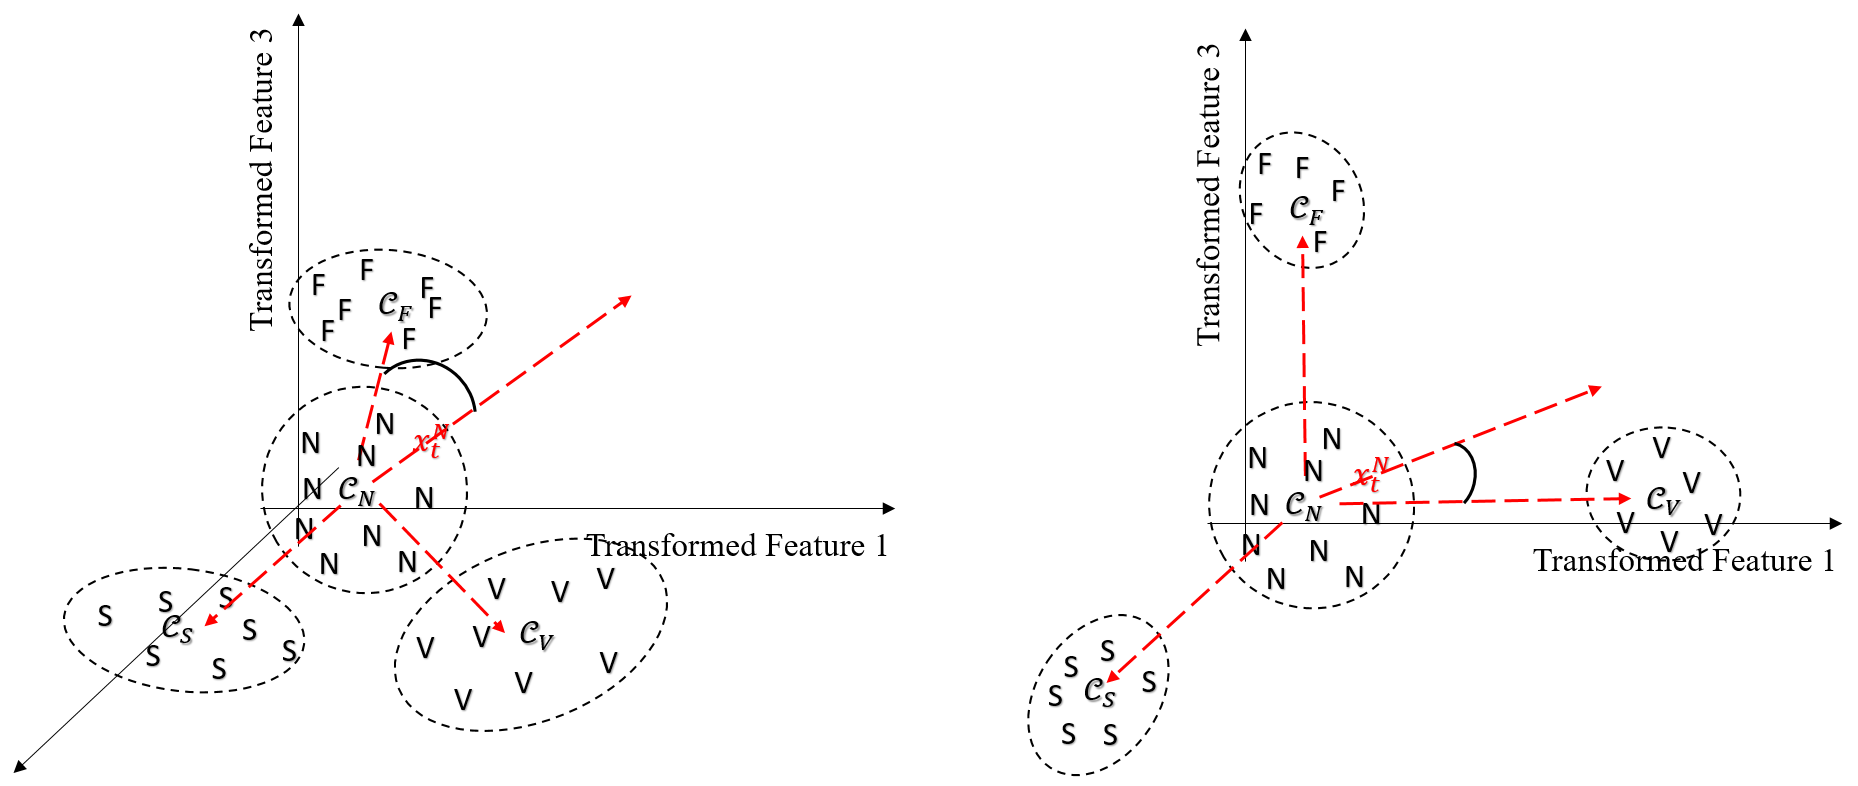
\includegraphics[scale=.42]{Fig/topo2.png}
\caption{Left: illustration of the clustering topology in the \textcolor{blue}{original} feature space; % transformed with a simple mapping function;  
Right: illustration of the clustering topology in the feature space transformed with an optimized mapping function. \textcolor{red}{Razi: it is not clear what you mean here by simple, is it unoptimized, why not just saying the original space before transmission !}}
\label{fig:topo2}
\end{figure}

\section{Hyper-Spherical Coordinates}

In the previous chapter, the spatial transformation module is implemented with a polynomial kernel function and a heuristic optimization method. The system performance has been proven to be promising. In addition to the general drawbacks of heuristic method, it is not straightforward to select an appropriate base kernel as the core of spatial mapping function due to the high variety of kernel functions. % and the limitation of dimensionality.

In order to address this issue, a novel deterministic spatial mapping function is proposed in this chapter based on \textit{hyper-spherical} coordinates [REF: XXX (it is ok to repeat references, ans is ok to have web pages as REFs)]. Since hyper-spherical coordinates consist of angles and radii, these parameters in both original feature space and the desired target space are used to determine the mapping function.


The hyper-spherical coordinate system (n-dimensional spherical coordinate system) and its mapping to the \textit{Cartesian} coordinate system are first introduced in \cite{nsphere}. If $\mathbf{x}$ is a sample vector in 
a $n$-dimensional feature space, with its Cartesian coordinates $(\xi_1,~\xi_2~... \xi_n)$, then its corresponding hyper-spherical coordinates can be obtained through Eq.\ref{eq:cart2sph}, which is originally derived through its reverse mapping (Eq.\ref{eq:sph2cart}) using equation: $\sin(\arccos(x)) = \sqrt{1-x^2}$.



\begin{align}
\label{eq:cart2sph}
\nonumber
r      &= \sqrt{{\xi_n}^2 + {\xi_{n-1}}^2 + \cdots + {\xi_2}^2 + {\xi_1}^2} \\
\nonumber
\theta_1 &= \arccos \frac{\xi_{1}}{\sqrt{{\xi_n}^2+{\xi_{n-1}}^2+\cdots+{\xi_1}^2}} \\
\nonumber
 \theta_2 &= \arccos \frac{\xi_{2}}{\sqrt{{\xi_n}^2+{\xi_{n-1}}^2+\cdots+{\xi_2}^2}} \\
\nonumber
        &\vdots\\
\nonumber
 \theta_{n-2} &=\arccos \frac{\xi_{n-2}}{\sqrt{{\xi_n}^2+{\xi_{n-1}}^2+{\xi_{n-2}}^2}} \\
 \theta_{n-1} &= 
 \begin{cases}
     \arccos \frac{\xi_{n-1}}{\sqrt{{\xi_n}^2+{\xi_{n-1}}^2}} & \xi_n\geq 0 \\
     - \arccos \frac{\xi_{n-1}}{\sqrt{{\xi_n}^2+{\xi_{n-1}}^2}} & \xi_n < 0
 \end{cases} 
\end{align}


\begin{align}
\label{eq:sph2cart}
\nonumber
\xi_1 &= r \cos(\theta_1) \\
%\xi_j &= r \cos(\theta_j)\prod_{k=1}^{j-1}\sin(\theta_k)\\
\nonumber
\xi_2 &= r \sin(\theta_1) \cos(\theta_2) \\
\nonumber
\xi_3 &= r \sin(\theta_1) \sin(\theta_2) \cos(\theta_3) \\
\nonumber
    &\vdots\\
\nonumber
\xi_{n-1} &= r \sin(\theta_1) \cdots \sin(\theta_{n-2}) \cos(\theta_{n-1}) \\
\xi_n &= r \sin(\theta_1) \cdots \sin(\theta_{n-2}) \sin(\theta_{n-1}).
\end{align}


where $0\leq \theta_j\leq\pi,~j=1,\dots ,n-2$; $0\leq \theta_{n-1}\leq 2 \pi$; $0\leq r<\infty$
 
 
\section{Orthogonalization}

To simplify the algorithm, in this chapter, the topology of clusters in the feature space is approximated by their centroid locations, \textcolor{blue}{denoted by $\mathbf{c}_N^k, \mathbf{c}_{\mathcal{V}}, \mathbf{c}_{\mathcal{S}}, \mathbf{c}_{\mathcal{F}}$, respectively for the normal cluster and the three abnormality clusters of type $V$, $S$, and $F$.} Furthermore, as we assume that the samples with fuzzy states deviate from the normal cluster to a specific abnormality cluster, the spatial topology stays unchanged if the normal centroid is simply translated to the origin of the Cartesian coordinate system. The clustering topology in the original feature space can be equivalently represented by the following matrix with three row vectors:

\begin{align}
\mathcal{C} = 
\begin{bmatrix}
\mathbf{c}_{\mathcal{V}} - \mathbf{c}_N^k \\
\mathbf{c}_{\mathcal{S}} - \mathbf{c}_N^k \\
\mathbf{c}_{\mathcal{F}} - \mathbf{c}_N^k
\end{bmatrix} = 
\begin{bmatrix}
\mathbf{v}_{\mathcal{VN}} \\
\mathbf{v}_{\mathcal{SN}} \\
\mathbf{v}_{\mathcal{FN}}
%\mathbf{v}_{\mathcal{VN}} \\
%\mathbf{v}_{\mathcal{SN}} \\
%\mathbf{v}_{\mathcal{FN}}
\end{bmatrix}
\end{align}
\textcolor{red}{RZ: I used lower case $v$ for vectors, which is more consistent with other definitions. Capital letter are more commonly used for matrices.}

As shown in Fig. \ref{fig:topo2}, in order to improve the performance of the personalized classifier and to avoid ambiguity in quantifying the deviations to different abnormality classes, a topology with a maximum separation between the three vectors of $\mathcal{C}$ is preferred. To achieve a lower computational complexity in higher order dimensions, the algorithm aims at transforming vectors in $\mathcal{C}$ to orthogonal vectors using a deterministic function. This approach not only simplifies the transformation derivations, it also ensures a full symmetry among abnormality clusters. As such, the problem reduces to finding a transformation that maps a set of vectors to a set of orthogonal vectors in the same space. Therefore, we can use the popular method of \textit{Gram-Schmidt} orthogonalization method \textcolor{blue}{RZ: introduced or explained, choose the right term} in \cite{Gram-schmidth1, Gram-schmidth2}. Hence, in the first step of this stage, the three row vectors of $\mathcal{C}$ representing the centroids of the three abnormality clusters are fed to the orthogonalization process as follows:
\begin{align}
\mathcal{C}^{\perp}= \text{Gram-Schmidt}(\mathcal{C})
=
\begin{bmatrix}
\mathbf{v}_{\mathcal{VN}}^{\perp} \\
\mathbf{v}_{\mathcal{SN}}^{\perp} \\
\mathbf{v}_{\mathcal{FN}}^{\perp},
\end{bmatrix}
\end{align}

where $\mathcal{C}^{\perp}$ is the matrix of orthogonalized vectors in the Cartesian coordinate system. The hyper-spherical coordinates $\mathcal{C}^{\perp}_{*}$ of these orthogonalized vectors are calculated subsequently using Eq.\ref{eq:cart2sph}. After this step, the orthogonalized vectors in the hyper-spherical coordinate system are obtained as formulated in Eq. \ref{eq:c_ortho}. The $j^{th}$ angular dimension denoted as  $\theta_{j}^{\perp}$ and the radius is noted as $r^{\perp}$.%, which reveals the angular change from original vectors to the ideal orthogonal vectors, are calculated subsequently using Eq.\ref{eq:cart2sph}.

\begin{align}
\label{eq:c_ortho}
\mathcal{C}^{\perp}_{*} =
\begin{bmatrix}
    r_{\mathcal{VN}}^{\perp} & \theta_{1_{\mathcal{VN}}}^{\perp} & \dots  & \theta_{{n-1}_{\mathcal{VN}}}^{\perp} \\
    r_{\mathcal{SN}}^{\perp} & \theta_{1_{\mathcal{SN}}}^{\perp} & \dots  & \theta_{{n-1}_{\mathcal{SN}}}^{\perp} \\
%    \vdots & \vdots & \ddots & \vdots \\
	r_{\mathcal{FN}}^{\perp} & \theta_{1_{\mathcal{FN}}}^{\perp} & \dots  & \theta_{{n-1}_{\mathcal{FN}}}^{\perp} \\
\end{bmatrix}
\end{align}


\section{Spatial Mapping Function}
After obtaining the original hyper-spherical coordinates of $[\mathbf{v}_{\mathcal{VN}},~\mathbf{v}_{\mathcal{SN}},~\mathbf{v}_{\mathcal{FN}}]^T$ and the orthogonalized hyper-spherical coordinates $[\mathbf{v}_{\mathcal{VN}}^{\perp},~\mathbf{v}_{\mathcal{SN}}^{\perp},~\mathbf{v}_{\mathcal{FN}}^{\perp}]^T$, the goal is to design a mapping function $\mathbf{F}: \mathbf{R}^n \to \mathbf{R}^n$ from the original coordinates to the orthogonal ones which exhibit the desired clustering topology, \textcolor{blue}{such that Equi. \ref{eq:constraints} holds.}

In the Gram-Schmidt algorithm, the very first vector serves as a reference vector and remains unchanged in the orthogonalization process, namely $\mathbf{v}_{\mathcal{VN}} = \mathbf{v}_{\mathcal{VN}}^{\perp}$. Therefore the mapping function $\mathbf{F}$ shall satisfy the following equations:

\begin{align}
\label{eq:constraints}
\begin{aligned}
%\mathbf{F}(0) &= 0 &~\\
\mathbf{F}(\mathbf{v}_{\mathcal{SN}} - \mathbf{v}_{\mathcal{VN}}) &= \mathbf{v}_{\mathcal{SN}}^{\perp} - \mathbf{v}_{\mathcal{VN}}^{\perp} &= \mathbf{v}_{\mathcal{SN}}^{\perp} - \mathbf{v}_{\mathcal{VN}}\\
\mathbf{F}(\mathbf{v}_{\mathcal{FN}} - \mathbf{v}_{\mathcal{VN}}) &= \mathbf{v}_{\mathcal{FN}}^{\perp} - \mathbf{v}_{\mathcal{VN}}^{\perp} &= \mathbf{v}_{\mathcal{FN}}^{\perp} - \mathbf{v}_{\mathcal{VN}}
\end{aligned}
\end{align}

Furthermore, since the orthogonality of vectors is independent to their radii $r$, we only need to design $\mathbf{F}$ for the $n-1$ angular dimensions ($\theta_1,\dots,\theta_{n-1}$), and the coordinate $r$ remains unchanged after the mapping. Consequently, the function $\mathbf{F}$ can be decomposed into $n-1$ functions: $f_i: \mathbf{R}\to \mathbf{R},~i=1\dots n-1$ with constraints in Eq.\ref{eq:constraints} as well as two additional extreme points defining the range of input and output values. %  \textcolor{red}{RZ: this part is not clear: and boundary constraints of angular dimensions, specified in Equi XXX: add equations for clarity.} 
%In order to standardize $f_i$ for all angular dimensions, $\theta_i, ~i=1\dots n-2$ are proportionally scaled to the range between $(0,2\pi)$.
We use the notation $\mathbf{v}_{\mathcal{SN}} - \mathbf{v}_{\mathcal{VN}} = \Delta_{\mathcal{SV}}$ and denote the the $i^{th}$ angular dimension of $\Delta_{\mathcal{SV}}$ as $\delta_{i_{{\mathcal{SV}}}}$. We use similar notations for the other dimensions, (e.g. $\mathbf{v}_{\mathcal{FN}} - \mathbf{v}_{\mathcal{VN}}$). %Hence for each angular dimension $i, i = 1,\dots, n-2$, $\delta_{i_{{\mathcal{SV}}}}$ and $\delta_{i_{{\mathcal{FV}}}}$ are both within the range of $(-\pi,\pi)$
Hence for each angular dimension $i$, $f_i$ is determined by ($\delta_{i_{{\mathcal{SV}}}}$,$\delta^{\perp}_{i_{{\mathcal{SV}}}}$) and ($\delta_{i_{{\mathcal{FV}}}}$,$\delta^{\perp}_{i_{{\mathcal{FV}}}}$), \textcolor{blue}{along with the two \textit{extreme boundary points} defining the domain and range of the functions.}



 %boundary constraints of angular dimensions. \textcolor{red}{RZ: Neads a little bit of clarification: by boundary constraints, do you mean the domain(input range) of the functions?. 2-Do you mean that $f_i$ should be designed such that it maps the two points () and () in the original space into points () and () in the target space?}
%if $f_i$ is to be depicted with a curve in 2-D plane, this curve will 4 points: (0,0), ($\delta_{i_{{\mathcal{SV}}}}$,$\delta^{\perp}_{i_{{\mathcal{SV}}}}$), ($\delta_{i_{{\mathcal{FV}}}}$,$\delta^{\perp}_{i_{{\mathcal{FV}}}}$), ($\pi$, $\pi$)

In order to maintain the simplicity and the linearity of the mapping function, the functions $f_i$ should be continuous and monotonic. For this purpose, the %\textcolor{red}{not clear:periodicity} 
valid range of angular dimensions (after considering the periodicity of these functions) is used to determine the boundary constrains; therefore the problem is transformed into a curve fitting problem. 

\textcolor{red}{RZ: the text was not clear, it now reads much better. }
\textcolor{blue}{For example, if linking ($\delta_{i_{{\mathcal{SV}}}}$,$\delta^{\perp}_{i_{{\mathcal{SV}}}}$) and ($\delta_{i_{{\mathcal{FV}}}}$,$\delta^{\perp}_{i_{{\mathcal{FV}}}}$) results in a monotonically increasing function, noting the fact that the range of $n-2$ first angular dimensions is the interval $[0, \pi]$, then the two extreme boundary points would be $(0,0)$ and $(\pi,\pi)$, as depicted in Fig. \ref{fig:simple_spline}. Conversely, for a monotonically increasing function, the extreme boundary points would be $(\pi,0)$ and $(0i,\pi)$. These rules apply for the functions defined for the $n-2$ first angular dimensions. 
Similar rules apply to the last angular dimension with only one consideration that the period is $2\pi$ instead of $\pi$. Since  ($\delta_{i_{{\mathcal{SV}}}}$,$\delta^{\perp}_{i_{{\mathcal{SV}}}}$) and ($\delta_{i_{{\mathcal{FV}}}}$,$\delta^{\perp}_{i_{{\mathcal{FV}}}}$) represent the orthogonalization process, they are decisive for this process. So we call these two points as well as the two extreme boundary points as \textit{target points} of the angular dimensions in the following sections.}

The simplest candidate function for $f_i$, which connects the two boundary points and the two target points in the 2-D plane would be a linear spline as shown in Fig.\ref{fig:simple_spline}.

%\textcolor{red}{RZ: I think, the concept of point and value and dimension mixed up here. A point in an Euclidean distance is defined by a vector (its values in different directions). Therefore, we should design a function that passes through two points (A,B) and (C,D). where A and B define the domain of function and B-D define the range of function in our case. We can discuss later to polish the text, or send me a clarification tonight. Anyway, we should complete the thesis by Monday and send the first version to the reviewers.}

\begin{figure}[t]
\centering
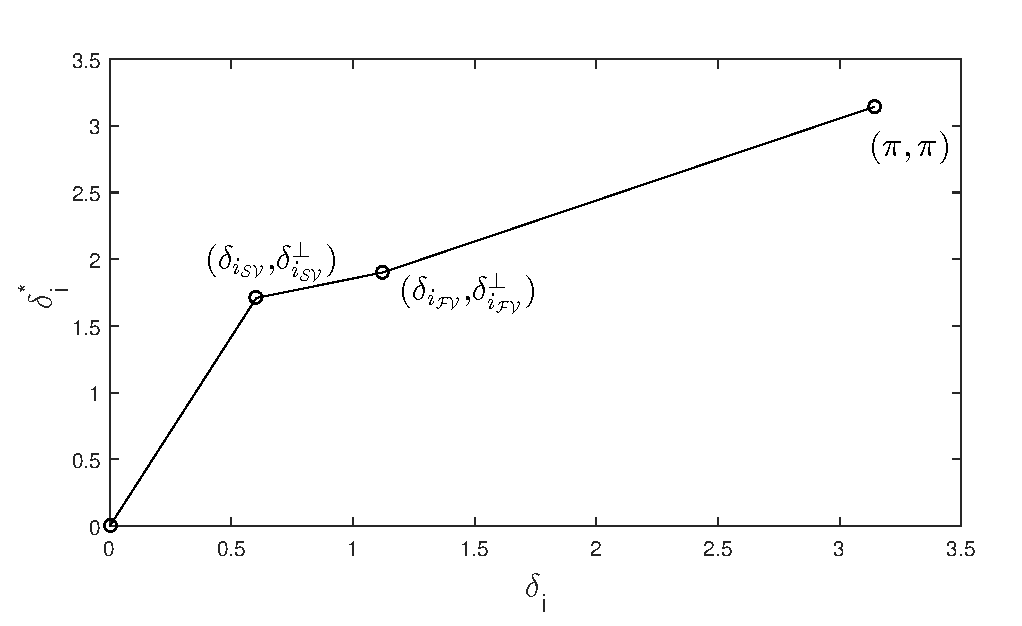
\includegraphics[scale=0.7]{Fig/simple_spline1.pdf}
\caption{\textcolor{blue}{The simple mapping function for one angular dimension which maps the target points in the original space to the desired target points. Target points include the two extreme boundary points $(0,0)$, and $\pi,\pi)$ as well as $(XXX,XXX)$ and $(XXX,XXX)$ to yield the desired mapping.} \textcolor{red}{add (0,0) and the label target and extreme boundary points to the figure.}}
%figure;plot([0,close,1.12,pi], [0,closed,1.9,pi],'-ko')
\label{fig:simple_spline}
\end{figure}

\section{Optimized Mapping Function}

The mapping function in Fig.\ref{fig:simple_spline} exhibits the two desired properties of monotonicity and continuity for an ideal mapping function $f_i$. However, this simple peicewise linear mapping function suffers from some drawbacks. Firstlt, the function is not differentiable at the target points ($\delta_{i_{{\mathcal{SV}}}}$,$\delta^{\perp}_{i_{{\mathcal{SV}}}}$) and ($\delta_{i_{{\mathcal{FV}}}}$,$\delta^{\perp}_{i_{{\mathcal{FV}}}}$), which can lead to severe cluster deformation. Secondly, the mapping function is applied to the angular dimensions, the discontinuity of the derivative of  %linearity of each spline in [RZ: I don't think, linearity causes this distortion.
the function can cause the convex-clusters to be mapped into non-convex clusters in the Cartesian coordinate system. In order to avoid deformations and to preserve maximal similarity with the original clustering geometry, it is desired to use a more linear functions with continuous derivatives. Also, in order to provide maximal separation among clusters and to concentrate clusters into disjoint non-overlapping clusters, it is beneficial to map the regions between two target points into a region with equal or even smaller range in the Cartesian coordinate system. In other words, it is desired to keep the samples close to the centroids in the mapped space as much as possible. This property is achieved by using nonlinear functions. However, there is a trade-off between the level of concentration and the linearity, which needs to be carefully addressed.  In order to avoid deformation while providing maximal separation, an optimized mapping function is proposed in this section.

In order to accommodate satisfy the above-mentioned requirements, it is desired to find a function, which satisfies the following mathematical conditions:

\begin{itemize}
\item the function is differentiable everywhere (continuous first derivative);
\item the derivative of the function is small at the target points, which correspond to the centroids of clusters in the original and transformed space, i.e. $\delta_{i_{{\mathcal{SV}}}}$ and $\delta_{i_{{\mathcal{FV}}}}$ in Fig. XXX;
\item the derivative of the function is large at the boundaries of two regions (\textcolor{blue}{point ($\epsilon_{i_{sv}},XXX))$ in Fig. XX.1.3};
\end{itemize}


Therefore, we propose to use the basis function $p$, which satisfies the aforementioned conditions. \textcolor{red}{why you call it basis function. Basis function has a different meaning in linear analysis. I suggest you use the term basic function with adjustable parameters.} Each target point is associated with a basic function. 
The function $p$ is composed of two constitutive functions: $h(x)$ and $g(x)$, \textcolor{blue}{respectively defined in two regions: i) from the target point to the upper boundary point, ii) from the lower boundary point to the next target point. [RZ: show h(x) and g(x) in Fig. 1.3.]. 
Before defining the two functions $h(x)$ and $g(x)$, we need to define the boundaries between two consecutive target points  ($\delta_{i_{{\mathcal{SV}}}}$,$\delta^{\perp}_{i_{{\mathcal{SV}}}}$) and ($\delta_{i_{{\mathcal{FV}}}}$,$\delta^{\perp}_{i_{{\mathcal{FV}}}}$), in which these functions are defined (i.g. $\epsilon_XXXX$). We simply choose the midpoint as the boundary points. For instance, we have $\epsilon=(\delta_1+\delta_2)/2$ [RZ:Write the correct equation] as stated in Equi. 1.7.
The lower and upper boundary points are denoted respectively as ($\gamma$,$\gamma^{\perp}$) and ($\epsilon$,$\epsilon^{\perp}$). To ensure the continuity of the mapping function $f$, the boundaries and target points should satisfy:}
 
%The boundaries that each function activates are decided by target points ($\delta_{i_{{\mathcal{SV}}}}$,$\delta^{\perp}_{i_{{\mathcal{SV}}}}$) and ($\delta_{i_{{\mathcal{FV}}}}$,$\delta^{\perp}_{i_{{\mathcal{FV}}}}$) along with the mid-points between the target points. The lower boundary mid points are noted as ($\gamma$,$\gamma^{\perp}$). The upper boundary mid points are noted as ($\epsilon$,$\epsilon^{\perp}$). To ensure the continuity of the mapping function $f$, the boundaries and target points satisfy:

\begin{align}
\begin{aligned}
(\epsilon_{i_{{\mathcal{SV}}}},\epsilon^{\perp}_{i_{{\mathcal{SV}}}}) &=
(\gamma_{i_{{\mathcal{FV}}}},\gamma^{\perp}_{i_{{\mathcal{FV}}}}) &=
(\frac{\delta_{i_{{\mathcal{SV}}}} + \delta_{i_{{\mathcal{FV}}}}}{2}, \frac{\delta^{\perp}_{i_{{\mathcal{SV}}}} + \delta^{\perp}_{i_{{\mathcal{FV}}}}}{2})
\end{aligned}
\end{align}

The two piece-wise functions $h(x)$ and $g(x)$ are defined as \textcolor{red}{use the correct name: the inverse of logit/sigmoid function} as follows:

\begin{align}
K_h &= \frac{\epsilon^{\perp}-\delta^{\perp}}{e^{\alpha(\epsilon-\delta,0)^{+}}-1}\\ \nonumber
h(x) &= K_h[e^{\alpha(x-\delta,0)^{+}}-1] + \delta^{\perp}
\end{align}
\begin{align}
K_g &= \frac{\gamma^{\perp}-\delta^{\perp}}{e^{\alpha(-\gamma+\delta,0)^{+}}-1}\\ \nonumber
g(x) &= K_g[e^{\alpha(\delta-x,0)^{+}}-1] + \delta^{\perp}
\end{align}

\fbox{RZ: revised up to here 2}.

To demonstrate this process, we first apply $p$ on two target points ($\delta_{i_{{\mathcal{SV}}}}$,$\delta^{\perp}_{i_{{\mathcal{SV}}}}$) and ($\delta_{i_{{\mathcal{FV}}}}$,$\delta^{\perp}_{i_{{\mathcal{FV}}}}$). This will result in a smooth curve as shown in Fig.\ref{fig:optimized_p}

\begin{figure}[t]
\centering
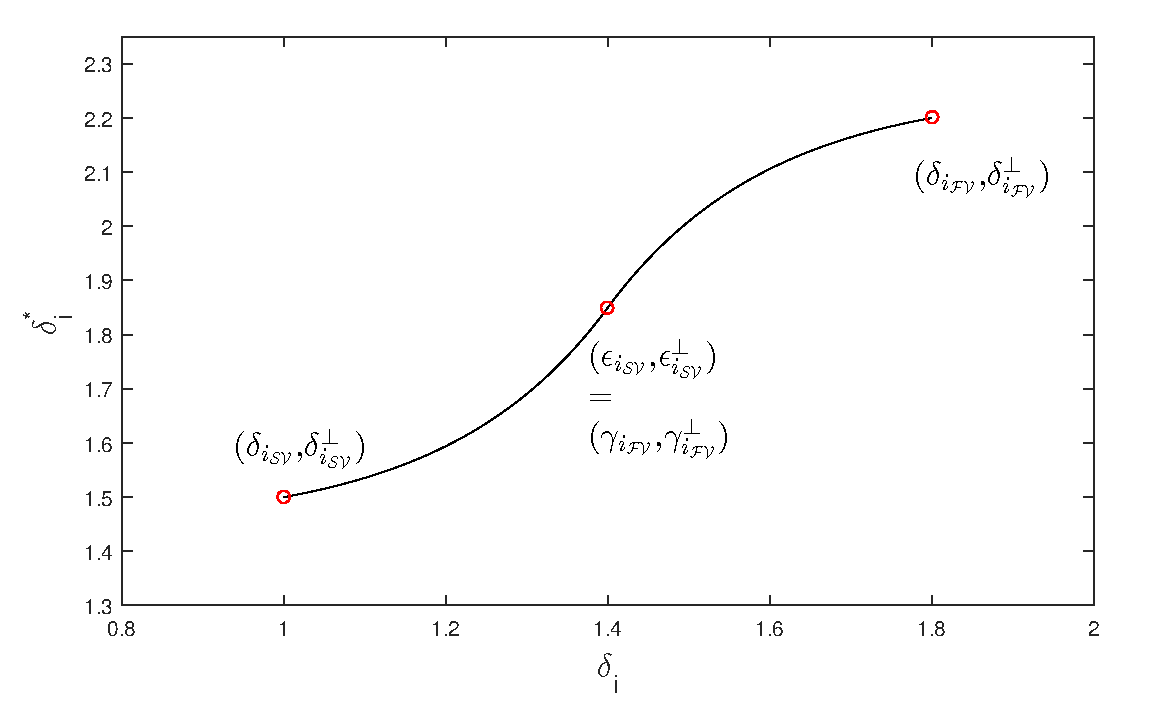
\includegraphics[scale=.7]{Fig/optimized_single_f.pdf}
\caption{Optimized Piece-wise Interpolated Function $p$. \textcolor{red}{I understand this figure, but is also misleading since the target points are at two ends and the boundary is in middle (the opposite is better). To solve this issue you can plot two adjacent regions and use tags and labels to show the target points $\delta$ and edge nodes/boundary nodes $\epsilon$}.}
\label{fig:optimized_p}
\end{figure}

Therefore, if we apply the piecewise interpolate function $p$ at all four target points: ($\delta_{i_{{\mathcal{SV}}}}$,$\delta^{\perp}_{i_{{\mathcal{SV}}}}$), ($\delta_{i_{{\mathcal{FV}}}}$,$\delta^{\perp}_{i_{{\mathcal{FV}}}}$) and two boundary points of angular dimension, the final result is shown in Fig.\ref{fig:optimized_map}

\begin{figure}[t]
\centering
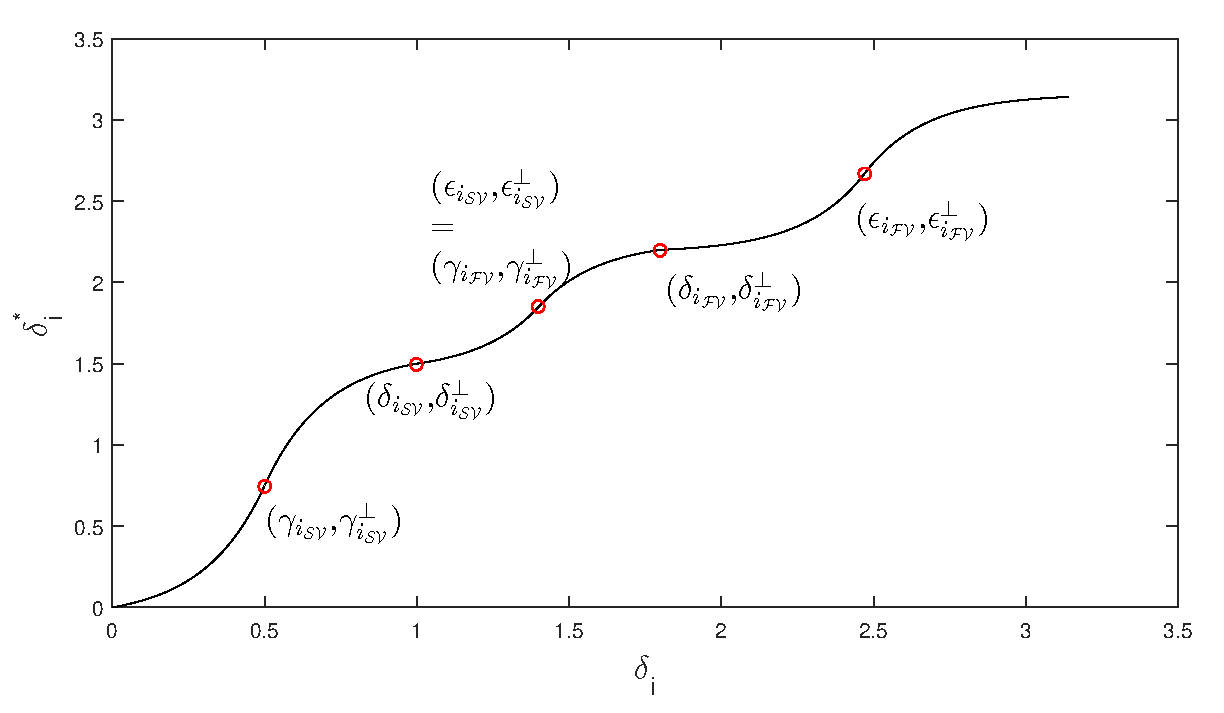
\includegraphics[scale=.7]{Fig/optimized_mapping_f.pdf}
\caption{Optimized Mapping Function $f$.}
\label{fig:optimized_map}
\end{figure}

In the training process, abnormal data from DS1 and personalized normal cluster are used to determine the mapping function. In the predicting process, the hyper-spherical coordinate of a new ECG sample is calculated and the mapping function is applied on its hyper-spherical coordinate. After this step, we calculate the Cartesian coordinate of the transformed data. This final result in Cartesian coordinate is then fed into Eq. \ref{eq:personal_discrim} to generate the corresponding type of yellow alarm.



\section{Experimental Results}\label{sec:result_spatial}

In this section, the performance of proposed method is evaluated according to two aspects. We will first analyze the classification performance of the system and demonstrate the comparison with other representative ECG classifiers. Furthermore, the classification results are partitioned into two sets:  red alarms generated by global classifier and final results by combining yellow and red alarms. In this way, the impacts of personalized classifier on final results can be revealed. Finally, the prediction performance which is representative in the proposed system is evaluated.

\subsection{Classification Performance}

The experimental results are evaluated with the classification performance of 4 AAMI ECG classes using the test subset of MITBIH Arrhythmia DS2. Originally DS2 contains 15357 samples after feature extraction. While training Personal Classifier, the first 20\% of total normal samples serve as initialization samples for personalized dynamic normal cluster. Therefore, all samples before the last initialization normal sample should be excluded from test set for each records. Consequently, the actual test set contains 12414 samples in total consisting of 10105 type-N, 1702 type-V, 508 type-S and 99 type-F samples.

To present the result, we select weighted k-Nearest Neighbors where $k=10$ as global classifier because it's comparatively simple and representative among low complexity models. The parameter $\alpha$ in the deviation detection module is set to 1 for test purpose. 

Table \ref{table:classification_cumu} summarized the cumulated confusion matrix for all records in the test set. In order to compare the result of global classifier and combined result, the sample numbers are presented in the following format: $combined(globaled)$. In order to measure classification performance, we adopted three metrics proposed in \cite{Hu_et_al,deChazal2006,ince2009generic}: accuracy($Ac$), sensitivity($Se$), specificity($Sp$). All three metrics are calculated based on true positive $TP$, false positive $FP$, false negative $FN$ and true negative $TN$ in a binary confusion matrix. Therefore all four metrics are calculated for each class by converting the 4x4 matrix to a 2x2 matrix.

\begin{table}[t]
	\centering
	\caption{Cumulated Confusion Matrix for All Records in DS2}
	\vspace{-0.05in}
	\begin{tabular}{|l|l|c|c|c|c|}
		\hline 
		&  \multicolumn{4}{c}{Ground Truth} &\\ 
        \hline
		\multirow{5}{*}{Result} &  & N & V & S & F  \\\cline{2-6}
		& N & 9255(10076)& 21(38) & 72(90) & 1(5) \\\cline{2-6} 
		&V & 657(22) & 1678(1663) & 8(2) & 9(7)  \\\cline{2-6}
		&S & 71(6) & 3(1) & 417(416) & 0(0)  \\\cline{2-6}
        &F& 122(1) & 0(0) & 11(0) & 89(87)  \\\hline
	\end{tabular}
	\label{table:classification_cumu} 
	\vspace{-0.15in}
\end{table}

While cumulated classification results are demonstrated in Table \ref{table:classification_cumu}, the robustness of the proposed method should be evaluated based on the performance variation over 22 test records in DS2. Hence medians and IQRs(interquartile range) for each metric and each class are included in Table \ref{table:variation} to represent the robustness of proposed methods. The lower variation between performances measured on different tapes, the more robust the system is. In Table \ref{table:variation}, we observe that among all abnormal classes, the proposed method demonstrates stable performance on class V but less stable on class S and F.

\begin{table}[b]
\centering
\caption{Classification Performance and Within-Set Variation of Proposed System}
\label{table:variation}
\resizebox{\textwidth}{!}{
\begin{tabular}{|c|c|c|c|c|c|c|c|c|c|c|c|c|}
\hline
\multirow{2}{*}{statistics} & \multicolumn{3}{c|}{N}                  & \multicolumn{3}{c|}{V}                  & \multicolumn{3}{c|}{S}                  & \multicolumn{3}{c|}{F}                  \\ \cline{2-13} 
                            & \textit{Ac} & \textit{Se} & \textit{Sp} & \textit{Ac} & \textit{Se} & \textit{Sp} & \textit{Ac} & \textit{Se} & \textit{Sp} & \textit{Ac} & \textit{Se} & \textit{Sp} \\ \hline
cumulated                   & 92.4        & 91.59       & 95.93       & 94.38       & 98.59       & 93.71       & 98.67       & 82.09       & 99.38       & 98.85       & 89.9        & 98.92       \\ \hline
median                      & 94.45       & 92.21       & 95.42       & 96.17       & 99.55       & 95.71       & 99.38       & 80.65       & 99.84       & 99.11       & 90.91       & 99.11       \\ \hline
IQR                         & 6.33        & 10.08       & 11.91       & 5.17        & 1.64        & 8.62        & 1.76        & 19.35       & 0.61        & 1.58        & 23.33       & 1.49        \\ \hline
\end{tabular}}
\end{table}

As MITDB is widely used to verify ECG classifier performance, we compared the proposed system with five significant methods proposed in literature. According to AAMI standards, ECG classifier performance should be evaluated over the binary classification performance of \textit{Ventricular (V)} versus \textit{non-V}types and \textit{Supraventricular (S)} versus \textit{non-S} types. For methods proposed in literature, same evaluation metrics are deployed on records from MITDB. To standardize the metrics, we select 11 common ECG records from all 5 methods and compared the median of each classification metrics over these 11 records. The comparison results are demonstrated in Table \ref{table:classification_comp}. Generally speaking, the proposed method shows higher sensitivity for both V type and S type. Especially for S type, the proposed method has advantage on all three metrics over other five methods in the literature.


\begin{table}[tbp]
\centering
\caption{V and S classification performance compared with five algorithms in literature using 11 common records in MITDB}
\label{table:classification_comp}
\begin{tabular}{|c|c|c|c|c|c|c|}
\hline
\multirow{2}{*}{Methods} & \multicolumn{3}{c|}{VEB} & \multicolumn{3}{c|}{SVEB} \\ \cline{2-7} 
                         & Ac     & Se     & Sp     & Ac      & Se     & Sp     \\ \hline
Proposed                 & 96.6   & 98.2   & 92.4   & 98.63   & 88.89  & 99.41  \\ \hline
Hu \textit{et al.}\cite{Hu_et_al}     & 94.8   & 78.9   & 96.8   & N/A     & N/A    & N/A    \\ \hline
de Chazal \textit{et al.}\cite{autofs}  & 96.4   & 77.5   & N/A    & N/A     & N/A    & N/A    \\ \hline
Jiang and Kong \cite{bbnn}    & 98.8   & 78.9   & 96.8   & 97.5    & 74.9   & 98.8   \\ \hline
Ince \textit{et al.} \cite{ince2009generic}    & 97.9   & 90.3   & 98.8   & 96.1    & 81.8   & 98.5   \\ \hline
Kiranyaz \textit{et al.}\cite{Kiranyaz}         & 98.9   & 95.9   & 99.4   & 96.4    & 68.8   & 99.5   \\ \hline
\end{tabular}
\end{table}

\subsection{Prediction Performance}

As an important characteristic of the proposed methods, yellow alarms triggered by personalized classifier after feature space reshaping indicate a higher probability of observing subsequent abnormalities. In order to verify this functionality, all beats following a yellow alarm is investigated for each yellow alarm. Abnormality type which occurs the earliest within the window is recorded. Similar to confusion matrix for classification evaluation, the performance of prediction can be summarized by a confusion matrix with the 3 abnormal types. Probabilities of observing a certain type of abnormal beats after a yellow alarm is calculated using the prediction confusion matrix and compared to the prior probability of observing the same type of abnormality. This process is formulated in the following two equations:

\begin{align}
\nonumber 
&P(\hat{y}_{k+i}=X_r|\hat{y}_{k}=X_y)=\frac{\text{\# of $y_{k+i}=X$ after $\hat{y}_k=X_y$}}{\text{\# of true alarms after $\hat{y}_k=X_y$}} \\
&P(\hat{y}_{k+i}=X_r)=\frac{\text{\# of true alarm of type $X$ ($y_{k}=X$)}}{\text{\# of all true alarms}} 
\end{align}

The power of predicting each type of abnormalities is evaluated by comparing $P(\hat{y}_{k+i}=X_r|\hat{y}_{k}=X_y)$ and $P(\hat{y}_{k+i}=X_r)$. A shown in Table \ref{table:pred}, the probability of observing a certain type of abnormalities after a yellow alarm is higher than its prior for each type of abnormalities. For example, without knowing the type of a yellow alarm, the probability of observing a type $V$ sample is 71.54\% while the probability of observing a type $V$ sample given a type $V$ yellow alarm was triggered is 77.45\%. The improvement are consistent among all three types of abnormalities but the system has stronger predicting capacity for type $S$. 

\begin{table}[t]
\centering
\caption{predictive probability versus prior probability without windowing}
\label{table:pred}
\begin{tabular}{|c|l|l|l|l||l|l|l|}
\hline
\multicolumn{2}{|l|}{\multirow{2}{*}{}} & \multicolumn{3}{l|}{\# of predicted ground truth} & \multicolumn{3}{l|}{\% of predicted ground truth} \\ \cline{3-8} 
\multicolumn{2}{|l|}{}                  & V               & S               & F             & V               & S               & F             \\ \hline
\multirow{3}{*}{yellow alarm}    & V    & 467             & 122              & 14            & \textbf{77.45}  & 20.23           & 2.32          \\ \cline{2-8} 
                                 & S    & 36              & 15              & 0             & 70.59           & \textbf{28.41}  & 0             \\ \cline{2-8} 
                                 & F    & 40              & 60              & 5             & 38.10           & 57.14           & \textbf{4.76} \\ \hline
\multicolumn{2}{|c|}{total}             & 543             & 197             & 19            & \textbf{71.54}  & \textbf{25.96}  & \textbf{2.50} \\ \hline
\end{tabular}
\end{table}

In order to study the time window in which real abnormality occurs after yellow alarms, we also studied a window of 10 consecutive samples following a yellow alarm. Similarly, prior and posterior probabilities are compared to evaluate the performance as shown in Table.\ref{table:pred10}. 


\begin{table}[t]
\centering
\caption{predictive probability versus prior probability within 10 beats' window}
\label{table:pred10}
\begin{tabular}{|c|l|l|l|l||l|l|l|}
\hline
\multicolumn{2}{|l|}{\multirow{2}{*}{}} & \multicolumn{3}{l|}{\# of predicted ground truth} & \multicolumn{3}{l|}{\% of predicted ground truth} \\ \cline{3-8} 
\multicolumn{2}{|l|}{}                  & V               & S               & F             & V               & S               & F             \\ \hline
\multirow{3}{*}{yellow alarm}    & V    & 290             & 85              & 12            & \textbf{74.94}  & 21.96           & 3.10          \\ \cline{2-8} 
                                 & S    & 22              & 13              & 0             & 62.86           & \textbf{37.14}  & 0             \\ \cline{2-8} 
                                 & F    & 29              & 37              & 6             & 40.28           & 51.39           & \textbf{8.33} \\ \hline
\multicolumn{2}{|c|}{total}             & 341             & 135             & 18            & \textbf{69.03}  & \textbf{27.32}  & \textbf{3.64} \\ \hline
\end{tabular}
\end{table}

Compared with the result without windowing, the predicting performance within 10 beats window shows that the proposed algorithm can better predict the occurrence of abnormalities in a certain time window. Especially for type S, the probability of observing a type S sample within 10 beats after a yellow alarm is 27.32\% while given that the yellow alarm is type S, the posterior probability is raise to 37.14\%. With almost 10\% increase, it's proved that the yellow alarm types are informative. The results shows that same improvements are made within the 10-sample window as well. In general, the predicting performance are promising, indicating the efficiency of personalized classifier and deviation analysis. %%\chapter{Controlled Spatial Transformation With Deterministic Mapping Function}
\section{Introduction}


 In Chapter 2, we elaborated on the details of patient adaptable ECG classification framework. In Chapter 3, the specific spatial topology of normal and abnormal clusters was analyzed in order to model the trajectory of ECG samples evolving from normal status to abnormal. These two methods share a common concept of modeling the intermediate states from annotated normal to abnormal state. 
 
 While the aforementioned systems demonstrated capacity of predicting upcoming abnormalities, it's challenging to interpret the mechanisms of the systems and thus hindering the generalization of predictive warning to other applications of biomedical signals. Therefore, the main object of this chapter is developing a classification system with abnormality predicting capacity based on spatial topology studied in \cite{chen2018predictive}. 
 
 Having analyzed the symmetric encircled topology in the previous chapter, we proposed a novel spatial transformation based predictive modeling system to assist cardiologist take advanced therapeutic Interventions. In this method, we further optimize the topology and spatial geometry of clusters in the feature space by reducing the within cluster variance after spatial transformation. As shown in \ref{fig:topo2}, through this improvement, the predicting accuracy of personal classifier can be further improved.
 
\begin{figure}[t]
\centering
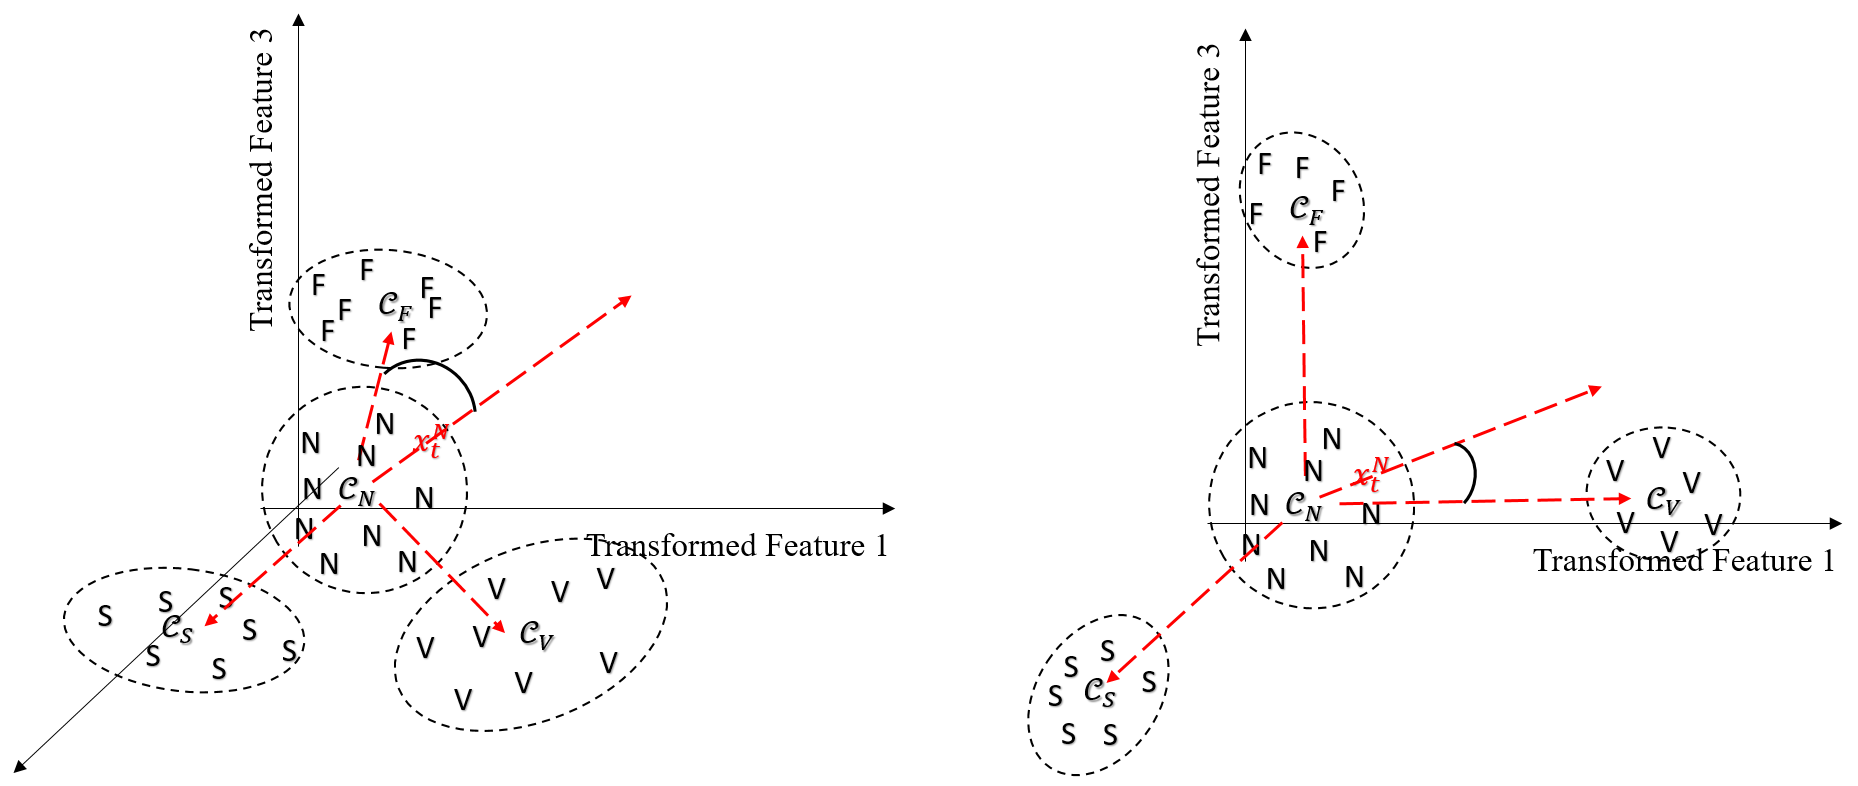
\includegraphics[scale=.42]{Fig/topo2.png}
\caption{Left: illustration of cluster topology in feature space transformed with simple mapping function; Right: illustration of cluster topology in feature space transformed with optimized mapping function}
\label{fig:topo2}
\end{figure}

\section{Hyper-Spherical Coordinates}

In the precedent chapter, the spatial transformation module was implemented with kernel function and heuristic optimization algorithm. The system performance was proved to be promising. However it's difficult to select the appropriate kernel as spatial mapping function due to the high variety of kernel functions and the limitation of dimensionality.

In order to address this problem, a novel deterministic spatial mapping function is proposed based on hyper-spherical coordinates in this work. Since hyper-spherical coordinates consists of angles and radius, this information together with the cluster topology are used to
determine the mapping function parameters.


Hyper-spherical coordinates (n-dimensional spherical coordinates) and its mapping to Cartesian coordinates are first elaborated in \cite{nsphere}. If $\mathbf{x}$ is a sample vector in 
$n$-dimensional feature space, where its Cartesian coordinates is $(\xi_1,~\xi_2~... \xi_n)$ , then its corresponding hyper-spherical coordinates can be obtained through Eq.\ref{eq:cart2sph} which is originally derived through its reverse mapping (Eq.\ref{eq:sph2cart}) using $\sin(\arccos(x)) = \sqrt{1-x^2}$



\begin{align}
\label{eq:cart2sph}
\begin{aligned}
r      &= \sqrt{{\xi_n}^2 + {\xi_{n-1}}^2 + \cdots + {\xi_2}^2 + {\xi_1}^2} \\
\theta_1 &= \arccos \frac{\xi_{1}}{\sqrt{{\xi_n}^2+{\xi_{n-1}}^2+\cdots+{\xi_1}^2}} \\
 \theta_2 &= \arccos \frac{\xi_{2}}{\sqrt{{\xi_n}^2+{\xi_{n-1}}^2+\cdots+{\xi_2}^2}} \\
        &\vdots\\
 \theta_{n-2} &=\arccos \frac{\xi_{n-2}}{\sqrt{{\xi_n}^2+{\xi_{n-1}}^2+{\xi_{n-2}}^2}} \\
 \theta_{n-1} &= 
 \begin{cases}
     \arccos \frac{\xi_{n-1}}{\sqrt{{\xi_n}^2+{\xi_{n-1}}^2}} & \xi_n\geq 0 \\
     - \arccos \frac{\xi_{n-1}}{\sqrt{{\xi_n}^2+{\xi_{n-1}}^2}} & \xi_n < 0
 \end{cases} 
 \end{aligned}
\end{align}


\begin{align}
\begin{aligned}
\label{eq:sph2cart}
\xi_1 &= r \cos(\theta_1) \\
%\xi_j &= r \cos(\theta_j)\prod_{k=1}^{j-1}\sin(\theta_k)\\
\xi_2 &= r \sin(\theta_1) \cos(\theta_2) \\
\xi_3 &= r \sin(\theta_1) \sin(\theta_2) \cos(\theta_3) \\
    &\vdots\\
\xi_{n-1} &= r \sin(\theta_1) \cdots \sin(\theta_{n-2}) \cos(\theta_{n-1}) \\
\xi_n &= r \sin(\theta_1) \cdots \sin(\theta_{n-2}) \sin(\theta_{n-1}) 
 .
\end{aligned}
\end{align}


where $0\leq \theta_j\leq\pi,~j=1,\dots ,n-2$; $0\leq \theta_{n-1}\leq 2 \pi$; $0\leq r<\infty$
 
 
\section{Orthogonalization}

To simplify algorithms, in this paper the topology of clusters in feature space is approximated by relative topology of cluster centroids: $\mathbf{c}_N^k, \mathbf{c}_{\mathcal{V}}, \mathbf{c}_{\mathcal{S}}, \mathbf{c}_{\mathcal{F}}$. Furthermore, as we assume that samples deviates from normality to abnormality and spatial topology stays unchanged if simple translation is applied to data, the cluster topology in original feature space can be simply represented by the following matrix:

\begin{align}
\mathcal{C} = 
\begin{bmatrix}
\mathbf{c}_{\mathcal{V}} - \mathbf{c}_N^k \\
\mathbf{c}_{\mathcal{S}} - \mathbf{c}_N^k \\
\mathbf{c}_{\mathcal{F}} - \mathbf{c}_N^k
\end{bmatrix} = 
\begin{bmatrix}
\mathbf{V}_{\mathcal{VN}} \\
\mathbf{V}_{\mathcal{SN}} \\
\mathbf{V}_{\mathcal{FN}}
\end{bmatrix}
\end{align}

As shown in Fig.\ref{fig:topo2}, in order to improve Personal Classifier and avoid ambiguity, a topology with maximum separation between three vectors in $\mathcal{C}$ is ideal. In order to lower computing complexity in high dimension, the algorithm aims at transforming vectors in $\mathcal{C}$ to orthogonal vectors with deterministic functions. Therefore, the method proposed in \cite{Gram-schmidth2} based on the well known orthogonalization method Gram-Schmidt in \cite{Gram-schmidth1} is deployed. Hence, in the first step of the function a vector of the centroids is fed to the orthogonalization process as follows:
\begin{align}
\mathcal{C}^{\perp}= \text{Gram-Schmidt}(\mathcal{C})
=
\begin{bmatrix}
\mathbf{V}_{\mathcal{VN}}^{\perp} \\
\mathbf{V}_{\mathcal{SN}}^{\perp} \\
\mathbf{V}_{\mathcal{FN}}^{\perp}
\end{bmatrix}
\end{align}

where $\mathcal{C}^{\perp}$ is the matrix of Cartesian coordinates orthogonalized vectors. The hyper-spherical coordinates $\mathcal{C}^{\perp}_{*}$ of same orthogonalized vectors, which reveals the angular change from original vectors to the ideal orthogonal vectors, are calculated subsequently using Eq.\ref{eq:cart2sph}.

\begin{align}
\mathcal{C}^{\perp}_{*} =
\begin{bmatrix}
    r_{\mathcal{VN}}^{\perp} & \theta_{1_{\mathcal{VN}}}^{\perp} & \dots  & \theta_{{n-1}_{\mathcal{VN}}}^{\perp} \\
    r_{\mathcal{SN}}^{\perp} & \theta_{1_{\mathcal{SN}}}^{\perp} & \dots  & \theta_{{n-1}_{\mathcal{SN}}}^{\perp} \\
%    \vdots & \vdots & \ddots & \vdots \\
	r_{\mathcal{FN}}^{\perp} & \theta{1_{\mathcal{FN}}}^{\perp} & \dots  & \theta_{{n-1}_{\mathcal{FN}}}^{\perp} \\
\end{bmatrix}
\end{align}


\section{Spatial Mapping Function}
After obtaining the original spherical coordinates ($\mathbf{V}_{\mathcal{VN}},~\mathbf{V}_{\mathcal{SN}},~\mathbf{V}_{\mathcal{FN}}$) and orthogonalized spherical coordinates ($\mathbf{V}_{\mathcal{VN}}^{\perp},~\mathbf{V}_{\mathcal{SN}}^{\perp},~\mathbf{V}_{\mathcal{FN}}^{\perp}$), the goal is to design a mapping function $\mathbf{F}: \mathbf{R}^n \to \mathbf{R}^n$ from original coordinates to the orthogonal ones which is equivalent to the ideal cluster topology.

In Gram-Schmidt algorithm, the very first vector in the input vector array serves as a reference vector and remains unchanged in the orthogonal vector array. As a result, $\mathbf{V}_{\mathcal{VN}} = \mathbf{V}_{\mathcal{VN}}^{\perp}$ and equivalently $\mathbf{F}$ can be defined by the following equations:

\begin{align}
\label{eq:constraints}
\begin{aligned}
%\mathbf{F}(0) &= 0 &~\\
\mathbf{F}(\mathbf{V}_{\mathcal{SN}} - \mathbf{V}_{\mathcal{VN}}) &= \mathbf{V}_{\mathcal{SN}}^{\perp} - \mathbf{V}_{\mathcal{VN}}^{\perp} &= \mathbf{V}_{\mathcal{SN}}^{\perp} - \mathbf{V}_{\mathcal{VN}}\\
\mathbf{F}(\mathbf{V}_{\mathcal{FN}} - \mathbf{V}_{\mathcal{VN}}) &= \mathbf{V}_{\mathcal{FN}}^{\perp} - \mathbf{V}_{\mathcal{VN}}^{\perp} &= \mathbf{V}_{\mathcal{FN}}^{\perp} - \mathbf{V}_{\mathcal{VN}}
\end{aligned}
\end{align}

Furthermore, since orthogonality is Independent to radius $r$, $\mathbf{F}$ only needs to apply to $n-1$ dimensions which includes all angles ($\theta_1,\dots,\theta_{n-1}$) and coordinate $r$ remains unchanged before and after mapping. Consequently, determination of $\mathbf{F}$ can be decomposed to the determination of $n-1$ functions: $f_i: \mathbf{R}\to \mathbf{R},~i=1\dots n-1$ with constraints in Eq.\ref{eq:constraints} and boundary constraints. %In order to standardize $f_i$ for all angular dimensions, $\theta_i, ~i=1\dots n-2$ are proportionally scaled to the range between $(0,2\pi)$.
Note the $\mathbf{V}_{\mathcal{SN}} - \mathbf{V}_{\mathcal{VN}}$ as $\Delta_{\mathcal{SV}}$ and its $i$th angular dimension of as $\delta_{i_{{\mathcal{SV}}}}$. Same notation is applied on $\mathbf{V}_{\mathcal{FN}} - \mathbf{V}_{\mathcal{VN}}$. %Hence for each angular dimension $i, i = 1,\dots, n-2$, $\delta_{i_{{\mathcal{SV}}}}$ and $\delta_{i_{{\mathcal{FV}}}}$ are both within the range of $(-\pi,\pi)$
Hence for each angular dimension $i$, $f_i$ is determined by ($\delta_{i_{{\mathcal{SV}}}}$,$\delta^{\perp}_{i_{{\mathcal{SV}}}}$) and ($\delta_{i_{{\mathcal{FV}}}}$,$\delta^{\perp}_{i_{{\mathcal{FV}}}}$), together with two boundary constraints
%if $f_i$ is to be depicted with a curve in 2-D plane, this curve will 4 points: (0,0), ($\delta_{i_{{\mathcal{SV}}}}$,$\delta^{\perp}_{i_{{\mathcal{SV}}}}$), ($\delta_{i_{{\mathcal{FV}}}}$,$\delta^{\perp}_{i_{{\mathcal{FV}}}}$), ($\pi$, $\pi$)
In order to maintain the simplicity and linearity of the mapping function, $f_i$ needs to be continuous and monotonic. For this purpose, periodicity of angular dimension is used to determine the boundary constrains and the problem is transformed into a curve fitting one. For example, if linking ($\delta_{i_{{\mathcal{SV}}}}$,$\delta^{\perp}_{i_{{\mathcal{SV}}}}$) and ($\delta_{i_{{\mathcal{FV}}}}$,$\delta^{\perp}_{i_{{\mathcal{FV}}}}$) results in a monotonically decreasing line, the boundary constrains would be $(\pi,0)$ and $(0,\pi)$. Conversely, if it results in a monotonically increasing line, the boundary constrains would be $(0,0)$ and $(\pi,\pi)$. Same rules applies on the last angular dimension where period is $2\pi$ instead of $pi$.

The simplest candidate function for $f_i$, which connect two boundary points and two target points in the 2-D plane would be a linear spline as shown in Fig.\ref{fig:simple_spline}

\begin{figure}[thpb]
\centering
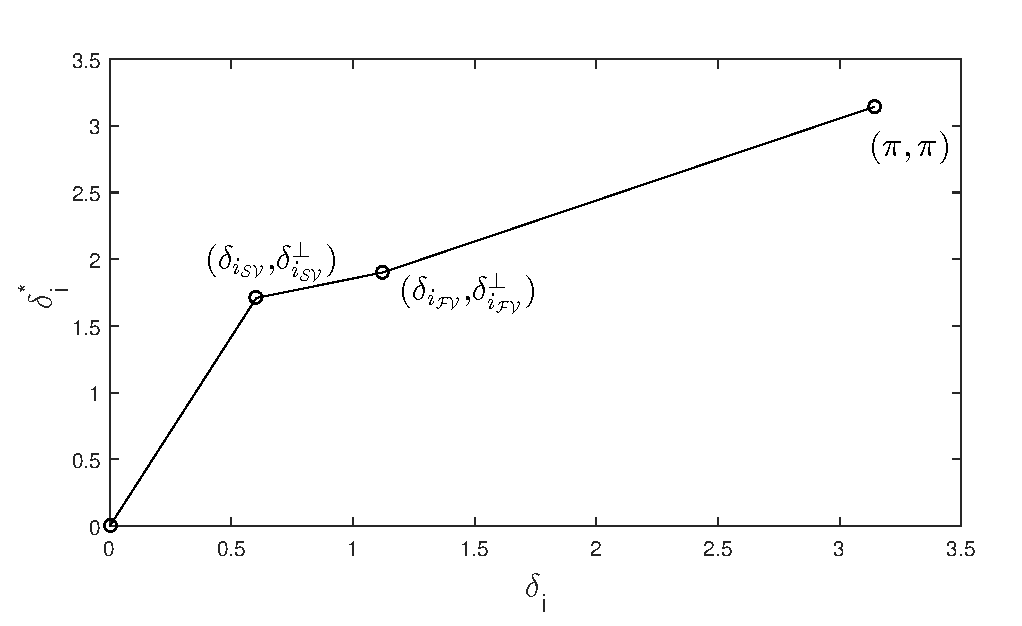
\includegraphics[scale=0.7]{Fig/simple_spline1.pdf}
\caption{The simple mapping function}
%figure;plot([0,close,1.12,pi], [0,closed,1.9,pi],'-ko')
\label{fig:simple_spline}
\end{figure}

\section{Optimized Mapping Function}

The mapping function in Fig.\ref{fig:simple_spline} demonstrated monotonicity and continuity, which is a part of targeted characteristics as an ideal mapping function for $f_i$. However there exists some drawbacks in the simple mapping function. First of all, the function is not differentiable at two target points ($\delta_{i_{{\mathcal{SV}}}}$,$\delta^{\perp}_{i_{{\mathcal{SV}}}}$) and ($\delta_{i_{{\mathcal{FV}}}}$,$\delta^{\perp}_{i_{{\mathcal{FV}}}}$), which will lead to cluster deformation. Secondly, since the mapping function is applied on angular dimension, linearity of each spline in the function will bring on non-convex clusters in Cartesian coordinates after mapping. In order to avoid deformations and preserve within cluster geometry, it is required to have a region for each cluster centroids within which the function maps the data to a equal or even smaller range in Cartesian coordinates. In the other word, the samples close to the centroids has to be close to the same corresponding centroids in the mapped space. In order to avoid deformations, an optimized mapping function is proposed.

To compromise three constrains, a function which satisfies the following mathematical conditions is studies:

\begin{itemize}
\item mapping function derivatives around centroids 0 and $\delta_{i_{{\mathcal{SV}}}}$ and $\delta_{i_{{\mathcal{FV}}}}$ are small
\item mapping function derivatives between two centroids large
\item quasi differentiable at all points
\end{itemize}

Therefore, we proposed the basis function $p$ satisfies the aforementioned constrains. The function $p$ is composed of two parts: $h(x)$ and $g(x)$. The boundaries that each function activates are defined as target points ($\delta_{i_{{\mathcal{SV}}}}$,$\delta^{\perp}_{i_{{\mathcal{SV}}}}$) and ($\delta_{i_{{\mathcal{FV}}}}$,$\delta^{\perp}_{i_{{\mathcal{FV}}}}$) along with the mid-points between target points. The lower boundary mid points are noted as ($\gamma$,$\gamma^{\perp}$). The upper boundary mid points are noted as ($\epsilon$,$\epsilon^{\perp}$). To ensure the continuity of mapping function $f$, we have

\begin{align}
\begin{aligned}
(\epsilon_{i_{{\mathcal{SV}}}},\epsilon^{\perp}_{i_{{\mathcal{SV}}}}) &=
(\gamma_{i_{{\mathcal{FV}}}},\gamma^{\perp}_{i_{{\mathcal{FV}}}}) &=
(\frac{\delta_{i_{{\mathcal{SV}}}} + \delta_{i_{{\mathcal{FV}}}}}{2}, \frac{\delta^{\perp}_{i_{{\mathcal{SV}}}} + \delta^{\perp}_{i_{{\mathcal{FV}}}}}{2})
\end{aligned}
\end{align}

Therefore, the two piecewise functions $h(x)$ and $g(x)$ are defined as follows:

\begin{align}
K_h &= \frac{\epsilon^{\perp}-\delta^{\perp}}{e^{\alpha(\epsilon-\delta,0)^{+}}-1}\\ \nonumber
h(x) &= K_h[e^{\alpha(x-\delta,0)^{+}}-1] + \delta^{\perp}
\end{align}
\begin{align}
K_g &= \frac{\gamma^{\perp}-\delta^{\perp}}{e^{\alpha(-\gamma+\delta,0)^{+}}-1}\\ \nonumber
g(x) &= K_g[e^{\alpha(\delta-x,0)^{+}}-1] + \delta^{\perp}
\end{align}

Applying $p$ on two target points ($\delta_{i_{{\mathcal{SV}}}}$,$\delta^{\perp}_{i_{{\mathcal{SV}}}}$) and ($\delta_{i_{{\mathcal{FV}}}}$,$\delta^{\perp}_{i_{{\mathcal{FV}}}}$) will result in a smooth curve as shown in Fig.\ref{fig:optimized_p}

\begin{figure}[thpb]
\centering
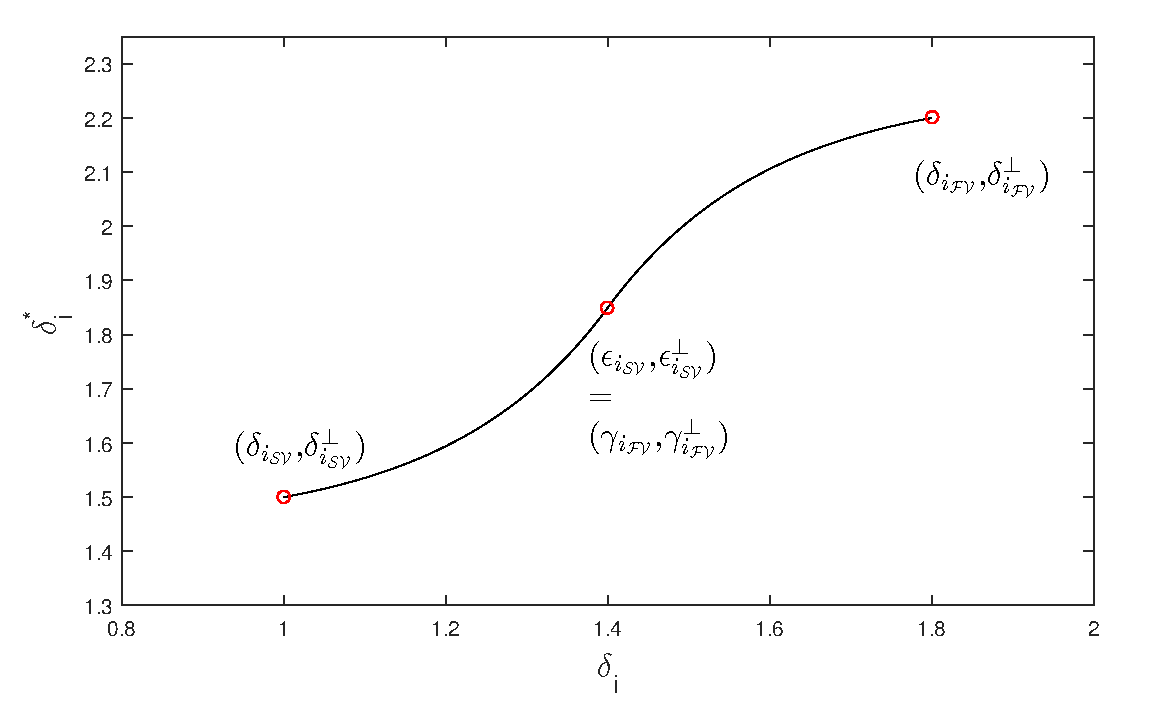
\includegraphics[scale=.7]{Fig/optimized_single_f.pdf}
\caption{Optimized Piecewise Interpolate Function $p$}
\label{fig:optimized_p}
\end{figure}

And applying the piecewise interpolate function $p$ at all four points: ($\delta_{i_{{\mathcal{SV}}}}$,$\delta^{\perp}_{i_{{\mathcal{SV}}}}$), ($\delta_{i_{{\mathcal{FV}}}}$,$\delta^{\perp}_{i_{{\mathcal{FV}}}}$) and two boundary points, the final result is shown in Fig.\ref{fig:optimized_map}

\begin{figure}[thpb]
\centering
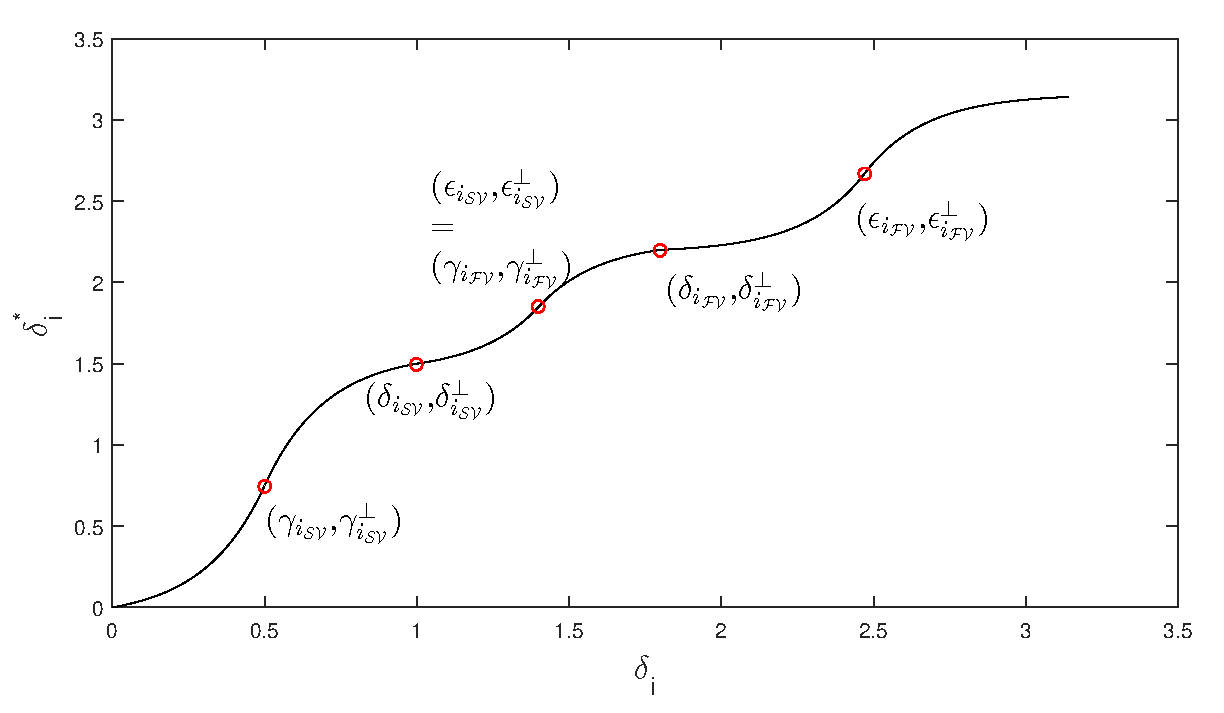
\includegraphics[scale=.7]{Fig/optimized_mapping_f.pdf}
\caption{Optimized Mapping Function $f$}
\label{fig:optimized_map}
\end{figure}

\section{Experimental Results}\label{sec:result_spatial}

In this section, the performance of proposed method is evaluated according to two aspects. We will first analyze the classification performance of the system and demonstrate the comparison with other representative ECG classifiers. Furthermore, the classification results are partitioned into two sets:   red alarms generated by Global Classifier and final results by combining yellow and red alarms. Impacts of Personal Classifier on final results will be studied. Finally the prediction performance which is typical in the proposed system is evaluated.

\subsection{Classification Performance}

The experimental results are evaluated with the classification performance of 4 AAMI ECG classes using the test subset of MITBIH Arrhythmia DS2. Originally DS2 contains 15357 samples after feature extraction. While training Personal Classifier, the first 20\% of total normal samples serve as initialization samples for Personal Dynamic Normal Cluster. Therefore, all samples before the last initialization normal sample should be excluded from test set for each records. Consequently  the actual test set contains 12414 samples in total consisting of 10105 type-N, 1702 type-V, 508 type-S and 99 type-F samples.

To present the result, we select weighted k-Nearest Neighbors where $k=10$ as Global Classifier as it's comparatively simple and representative among low complexity models. Parameter $\alpha$ in the deviation detection module is set to 1 for test purpose. 

Table \ref{table:classification_cumu} summarized the cumulated confusion matrix for all records in the test set. In order to compare the result of Global Classifier and combined result, the sample numbers are presented in the following format: $combined(globaled)$. In order to measure classification performance, we adopted four metrics proposed in \cite{Hu_et_al}: accuracy($Ac$), sensitivity($Se$), specificity($Sp$) and precision($Pr$). All four metrics are calculated based on true positive $TP$, false positive $FP$, false negative $FN$ and true negative $TN$ in a binary confusion matrix. Therefore all four metrics are calculated for each class by converting the 4x4 matrix to a 2x2 matrix.

\begin{table}[t]
	\centering
	\caption{Cumulated Confusion Matrix for All Records in DS2}
	\vspace{-0.05in}
	\begin{tabular}{|l|l|c|c|c|c|}
		\hline 
		&  \multicolumn{4}{c}{Ground Truth} &\\ 
        \hline
		\multirow{5}{*}{Result} &  & N & V & S & F  \\\cline{2-6}
		& N & 9255(10076)& 21(38) & 72(90) & 1(5) \\\cline{2-6} 
		&V & 657(22) & 1678(1663) & 8(2) & 9(7)  \\\cline{2-6}
		&S & 71(6) & 3(1) & 417(416) & 0(0)  \\\cline{2-6}
        &F& 122(1) & 0(0) & 11(0) & 89(87)  \\\hline
	\end{tabular}
	\label{table:classification_cumu} 
	\vspace{-0.15in}
\end{table}

While cumulated classification results are demonstrated in Table \ref{table:classification_cumu}, the robustness of the proposed method should be evaluated based on the performance variation over 22 test records in DS2. Hence medians and IQRs(interquartile range) for each metric and each class are included in Table \ref{table:variation} to represent the robustness of proposed methods. The lower variation between performances measured on different tapes, the more robust the system is. In Table \ref{table:variation}, we observe that among all abnormal classes, the proposed algorithms demonstrated stable performance on class V and high performance but less stable on class V and F.

\begin{table}[]
\centering
\caption{Classification Performance and Within-Set Variation of Proposed System}
\label{table:variation}
\resizebox{\textwidth}{!}{
\begin{tabular}{|c|c|c|c|c|c|c|c|c|c|c|c|c|}
\hline
\multirow{2}{*}{statistics} & \multicolumn{3}{c|}{N}                  & \multicolumn{3}{c|}{V}                  & \multicolumn{3}{c|}{S}                  & \multicolumn{3}{c|}{F}                  \\ \cline{2-13} 
                            & \textit{Ac} & \textit{Se} & \textit{Sp} & \textit{Ac} & \textit{Se} & \textit{Sp} & \textit{Ac} & \textit{Se} & \textit{Sp} & \textit{Ac} & \textit{Se} & \textit{Sp} \\ \hline
cumulated                   & 92.4        & 91.59       & 95.93       & 94.38       & 98.59       & 93.71       & 98.67       & 82.09       & 99.38       & 98.85       & 89.9        & 98.92       \\ \hline
median                      & 94.45       & 92.21       & 95.42       & 96.17       & 99.55       & 95.71       & 99.38       & 80.65       & 99.84       & 99.11       & 90.91       & 99.11       \\ \hline
IQR                         & 6.33        & 10.08       & 11.91       & 5.17        & 1.64        & 8.62        & 1.76        & 19.35       & 0.61        & 1.58        & 23.33       & 1.49        \\ \hline
\end{tabular}}
\end{table}

As MITDB is widely used to verify ECG classifier performance, we compared the proposed system with five significant methods proposed in literature. According to AAMI standards, ECG classifier performance should be evaluated over the binary classification performance of Ventricular (VEB) versus non-VEB types and Supraventricular(SVEB) versus non-SVEB types. For methods proposed in literature, same evaluation metrics are deployed on records from MITDB. To standardize the metrics, we select 11 common ECG records from all 5 methods and compared the median of each classification metrics over these 11 records. The comparison results are demonstrated in Table.\ref{table:classification_comp}. Generally speaking, the proposed method shows higher sensitivity for both VEB and SVEB. Especially for SVEB, the proposed method has advantage on all three metrics over other five methods in the literature.


\begin{table}[tbp]
\centering
\caption{V and S classification performance compared with five algorithms in literature using 11 common records in MITDB}
\label{table:classification_comp}
\begin{tabular}{|c|c|c|c|c|c|c|}
\hline
\multirow{2}{*}{Methods} & \multicolumn{3}{c|}{VEB} & \multicolumn{3}{c|}{SVEB} \\ \cline{2-7} 
                         & Ac     & Se     & Sp     & Ac      & Se     & Sp     \\ \hline
Proposed                 & 96.6   & 98.2   & 92.4   & 98.63   & 88.89  & 99.41  \\ \hline
Hu \textit{et al.}\cite{Hu_et_al}     & 94.8   & 78.9   & 96.8   & N/A     & N/A    & N/A    \\ \hline
de Chazal \textit{et al.}\cite{autofs}  & 96.4   & 77.5   & N/A    & N/A     & N/A    & N/A    \\ \hline
Jiang and Kong \cite{bbnn}    & 98.8   & 78.9   & 96.8   & 97.5    & 74.9   & 98.8   \\ \hline
Ince \textit{et al.} \cite{ince2009generic}    & 97.9   & 90.3   & 98.8   & 96.1    & 81.8   & 98.5   \\ \hline
Kiranyaz \textit{et al.}\cite{Kiranyaz}         & 98.9   & 95.9   & 99.4   & 96.4    & 68.8   & 99.5   \\ \hline
\end{tabular}
\end{table}

\subsection{Prediction Performance}

As an important characteristic of the proposed methods, yellow alarms triggered by Personal Classifier after feature space reshaping indicate a higher probability of observing subsequent abnormalities. In order to verify this functionality, all beats following a yellow alarm is investigated for each yellow alarm. Abnormality type which occurs the earliest within the window is recorded. Similar to confusion matrix for classification evaluation, the performance of prediction can be summarized by a confusion matrix with the 3 abnormal types. Probabilities of observing an certain type of abnormal beats after a yellow alarm is calculated using the prediction confusion matrix and compared to the prior probability of observing the same type of abnormality. This process is formulated in the following two equations:

\begin{align}
\nonumber 
&P(\hat{y}_{k+i}=X_r|\hat{y}_{k}=X_y)=\frac{\text{\# of $y_{k+i}=X$ after $\hat{y}_k=X_y$}}{\text{\# of true alarms after $\hat{y}_k=X_y$}} \\
&P(\hat{y}_{k+i}=X_r)=\frac{\text{\# of true alarm of type $X$ ($y_{k}=X$)}}{\text{\# of all true alarms}} 
\end{align}

The capacity of predicting each type of abnormalities is evaluated by comparing $P(\hat{y}_{k+i}=X_r|\hat{y}_{k}=X_y)$ and $P(\hat{y}_{k+i}=X_r)$. A shown in Table.\ref{table:pred}, the probability of observing a certain type of abnormalities after a yellow alarm are higher than its prior for each type of abnormalities. For example, without knowing the type of a yellow alarm, the probability of observing a type $V$ sample is 71.54\% while the probability of observing a type $V$ sample given a type $V$ yellow alarm was triggered is 77.45\%. The improvement are consistent among all three types of abnormalities but the system has stronger predicting capacity for type $S$. 

\begin{table}[t]
\centering
\caption{predictive probability versus prior probability without windowing}
\label{table:pred}
\begin{tabular}{|c|l|l|l|l||l|l|l|}
\hline
\multicolumn{2}{|l|}{\multirow{2}{*}{}} & \multicolumn{3}{l|}{\# of predicted ground truth} & \multicolumn{3}{l|}{\% of predicted ground truth} \\ \cline{3-8} 
\multicolumn{2}{|l|}{}                  & V               & S               & F             & V               & S               & F             \\ \hline
\multirow{3}{*}{yellow alarm}    & V    & 467             & 122              & 14            & \textbf{77.45}  & 20.23           & 2.32          \\ \cline{2-8} 
                                 & S    & 36              & 15              & 0             & 70.59           & \textbf{28.41}  & 0             \\ \cline{2-8} 
                                 & F    & 40              & 60              & 5             & 38.10           & 57.14           & \textbf{4.76} \\ \hline
\multicolumn{2}{|c|}{total}             & 543             & 197             & 19            & \textbf{71.54}  & \textbf{25.96}  & \textbf{2.50} \\ \hline
\end{tabular}
\end{table}

In order to study the time window in which real abnormality occurs after yellow alarms, we also studied a window of 10 consecutive samples following a yellow alarm. Similarly, prior and posterior probabilities are compared to evaluate the performance as shown in Table.\ref{table:pred10}. 


\begin{table}[t]
\centering
\caption{predictive probability versus prior probability within 10 beats' window}
\label{table:pred10}
\begin{tabular}{|c|l|l|l|l||l|l|l|}
\hline
\multicolumn{2}{|l|}{\multirow{2}{*}{}} & \multicolumn{3}{l|}{\# of predicted ground truth} & \multicolumn{3}{l|}{\% of predicted ground truth} \\ \cline{3-8} 
\multicolumn{2}{|l|}{}                  & V               & S               & F             & V               & S               & F             \\ \hline
\multirow{3}{*}{yellow alarm}    & V    & 290             & 85              & 12            & \textbf{74.94}  & 21.96           & 3.10          \\ \cline{2-8} 
                                 & S    & 22              & 13              & 0             & 62.86           & \textbf{37.14}  & 0             \\ \cline{2-8} 
                                 & F    & 29              & 37              & 6             & 40.28           & 51.39           & \textbf{8.33} \\ \hline
\multicolumn{2}{|c|}{total}             & 341             & 135             & 18            & \textbf{69.03}  & \textbf{27.32}  & \textbf{3.64} \\ \hline
\end{tabular}
\end{table}

Compared with the result without windowing, the predicting performance within 10 beats window shows that the proposed algorithm can better predict the occurrence of abnormalities in a centrain time window. Especially for type S, the probability of observing a type S sample within 10 beats after a yellow alarm is 27.32\% while given that the yellow alarm is type S, the posterior probability is raise to 37.14\%. With almost 10\% increase, it's proved that the yellow alarm types are informative. The results shows that same improvements are made within the 10-sample window as well. In general, the predicting performance are promising, indicating the efficiency of personal classifier and deviation analysis.
%\include{body/5-learning}
% \chapter{Conclusions And Future works} \label{ch:Discussion And Resuls}
 
\section{Conclusions}
In this thesis, we a patient-adaptable ECG classification framework. The system has a two-staged hierarchical classifier structure including Global Classifier and Personal Classifier. While Global Classifier is designed to filter the signal with severe distortion and abnormal waveforms by triggering red alarms and pass other samples to the deviation detection stage. In this stage, the personal dynamic normal cluster is constructed and used to specify the normal range for each patient. By comparing the current sample and personalized normal range, this module decides if a yellow alarm will be triggered to provide predictive information about upcoming abnormalities. If a sample is detected with deviation towards abnormal clusters, it will be passed to the Personal Classifier and labeled as one of the three abnormal types. Whereas samples without deviation are further feed back to personal dynamic normal cluster to update the classification system about the newest personal normal range.

In Chapter 3, a kernel based nonlinear transformation is proposed to address the problem of cluster topology in original feature space. Inspired by Support Vector Machine, kernel functions are deployed in this method as a spatial transformation function. The target topology is formulated as two objective functions so that by tuning the parameters in kernel function, the system is able to select the best transformation for the following predicting stage. This non-convex multi-objective optimization is solved with Multi-Objective Particle Swarm Optimization. In order to validate improvement by using high order kernel function, we compared the Pareto front generated with linear combination of original features and mapped high order features with polynomial kernel. The result verifies that applying high order kernel function allows more degree of freedom so that the topology can be further optimized according to objective functions. Having this concept proved, we applied this method on MITDB test data and obtained similar sensitivity and specificity as proposed in the literatures. More importantly, the predicting capacity of yellow alarms are analyzed. The performance is quantified by comparing prior probability and posterior probability giving the types of yellows alarm. The comparison result shows that a promising improvement has been made by applying the nonlinear transformation. 

While the method in Chapter 3 demonstrated capacity of predicting upcoming abnormalities, it's challenging to interpret the mechanisms of the systems and thus hindering the generalization of predictive warning to other applications of biomedical signals. Therefore, the main object of Chapter 4 is developing a classification system with abnormality predicting capacity based on spatial topology studied in Chapter 3. In Chapter 4, we proposed a novel spatial transformation specifically designed to reshape the feature space according to angles between cluster center. In this method, between cluster cosine distance are optimized through orthogonalization in spherical coordinate space and within cluster variance is reduced by a mapping function which is fitted piecewise with a basis function. The basis function proposed in the chapter has the feature of saturating at the boundaries, similar to sigmoid function but more flexible. An advantage of deploying such basis function is that the cluster geometry may be preserved after spatial transformation. With this novel module integrated in the patient-adaptable classification framework, the performance of this system is evaluated through classification and prediction results on the test set data. The classification results show that by triggering yellow alarm through this method, specificity of abnormal types is improved. Especially for Supraventricular types, the proposed system performs better than all 5 methods in the literature. The same conclusion holds for prediction performance. Compared to the method proposed in Chapter 3, this method improves predicting capacity for all abnormal classes and the most significant improvement is for type S. Moreover, we also studied the time delay of real abnormalities following a yellow alarm. It's proved that most of the real abnormalities occurs within 10 beat after a yellow alarm. Generally speaking, the system is proved to be efficient both in classification and prediction.


\section{Future works}
In this research, we focused on two challenges of ECG classification, namely, inter-patient variation and anomaly prediction. The framework of patient-adaptable classier includes both features. The methods of improving prediction accuracy are proposed and studied. While the result shows the efficiency of designed system, further improvements can be made through research. The following tasks can be resolved as a continuation of this research:
 \begin{itemize}
\item Research on other kernel functions which is potentially a better transformation for spatial topology optimization.
\item Investigate on the deterministic solution for the objective functions proposed in Chapter 3.
\item Assess the performance of proposed spatial transformation on other biomedical signals with similar characters as ECG signal
\item  Improve the deterministic mapping function in Chapter 4 by including the variance of individual clusters into function parameters
\end{itemize}


%\include{conclusion/6-Result}
%%%%%%%%%%%%%%%%%%%%%%%%%%%%%%%%
%\chapter{References}
%\printbibliography[heading=none]
\bibliographystyle{ieeetr}
\bibliography{Bibs}
% If you are using BibTeX, uncomment the following:
%\thebibliography
%
% Otherwise, uncomment the following:
% \chapter*{Bibliography}
% \appendix

% In LaTeX, each appendix is a "chapter"
% \chapter{Program Source}


\end{document}
